\documentclass[UTF8,fontset=windows,11pt]{ctexart}
\usepackage[a4paper,margin=2.35cm]{geometry}
\usepackage{amsmath,amssymb,bm,mathtools}
\usepackage{booktabs,longtable,array}
\usepackage{graphicx}
\graphicspath{{figures/v7/}}
\usepackage[section]{placeins}
\usepackage{xcolor}
\usepackage{enumitem}
\usepackage{algorithm}
\usepackage{algpseudocode}
\usepackage{amsthm}
\usepackage{caption}
\captionsetup{font=small,labelfont=bf,labelsep=quad,skip=6pt}
\setlength{\textfloatsep}{14pt plus 3pt minus 3pt}
\setlength{\floatsep}{12pt plus 2pt minus 2pt}
\renewcommand{\topfraction}{0.92}
\renewcommand{\bottomfraction}{0.85}
\renewcommand{\textfraction}{0.07}
\renewcommand{\floatpagefraction}{0.72}
\setcounter{topnumber}{3}
\setcounter{totalnumber}{5}
\raggedbottom
\ctexset{section={format=\Large\bfseries\raggedright},subsection={format=\large\bfseries\raggedright}}
\makeatletter
\renewcommand{\maketitle}{\begin{center}\vspace*{-1em}{\LARGE\bfseries\noindent\@title\par}\vspace{1em}\end{center}}
\makeatother
\usepackage{hyperref}
\usepackage{microtype}
\newcommand{\upcite}[1]{\textsuperscript{\cite{#1}}}
\floatname{algorithm}{算法}
\newtheorem{theorem}{定理}[section]
\newtheorem{proposition}[theorem]{命题}
\newtheorem{lemma}[theorem]{引理}
\newtheorem{corollary}[theorem]{推论}
\newtheorem{definition}[theorem]{定义}
\newcommand{\Sone}{\mathbb S^1}
\newcommand{\Ttwo}{\mathbb T^2}
\newcommand{\E}{\mathbb E}
\newcommand{\R}{\mathbb R}
\algrenewcommand\algorithmicrequire{\textbf{输入：}}
\algrenewcommand\algorithmicensure{\textbf{输出：}}
\algrenewcommand\algorithmicfor{\textbf{对于}}
\algrenewcommand\algorithmicdo{\textbf{执行}}
\algrenewcommand\algorithmicend{\textbf{结束}}
\algrenewcommand\algorithmicreturn{\textbf{返回}}
\hypersetup{colorlinks=true,linkcolor=black,citecolor=black,urlcolor=blue,
 pdftitle={间歇观测下异中心神经场的卡尔曼滤波补偿},
 pdfsubject={异中心神经场集群运动与Kalman预测补偿},
 pdfkeywords={异中心表征；环形吸引子；集群运动；间歇观测；Kalman滤波},
 bookmarksnumbered=true}
\setlength{\parindent}{2em}
\setlength{\parskip}{0.12em}
\linespread{1.10}
\setlength{\emergencystretch}{1em}
\title{间歇观测下异中心神经场的卡尔曼滤波补偿}
\author{}
\date{}
\begin{document}
\maketitle

\begin{abstract}
邻居方位的间歇缺失会改变异中心神经场的社会输入，并通过神经活动和运动反馈影响群体协同。本文围绕输入量化、预测重建和群体响应三个挑战，建立从局部观测到集群运动的卡尔曼滤波补偿框架。首先，以邻居数量、单边强度和二维合方向描述社会输入，比较指数、带基线余弦等六类正值形式，综合评价二维运动与神经活动的预测精度。在 $400$ 组独立测试几何的 $9600$ 个条件中，所选无额外角度衰减形式的速度和活动 RMSE 较固定指数分别降低 $2.36\%$ 和 $4.17\%$。其次，构建新鲜观测直通、方位--角速度预测与协方差感知周期输入相结合的重建方法，建立后验输入重建、方向信息衰减与有限时间扰动传播的理论联系。五种子开发实验中，中心条件的同状态输入误差较方位保持降低 $61.8\%$；进一步设计共同样本下的预测精度、协方差校准与输入重建分层实验。最后，采用共同检查点分叉和配对统计，以有序度与凝聚距离评价补偿对群体运动的作用。三十种子遮挡与受控转向实验表明，历史信息延续降低了相对无遮挡参考的行为偏差，方向预测的增量随时长和指标变化；后续在分层重建实验确定配置后，沿新鲜输入数量、方位结构和缺失时长开展条件边界评价。三条主线分别连接输入表达、信息延续与群体协同，为间歇观测下的神经场补偿提供统一研究路径。

\end{abstract}

\noindent\textbf{关键词：} 异中心表征；环形吸引子；集群运动；间歇观测；Kalman滤波；方位预测；不确定性传播

\section{引言}

局部感知约束是分布式集群运动的重要问题。有限视场下的多无人机控制需要协调邻居感知与排斥行为\upcite{Bai2024}，林下集群导航需要处理环境不确定性\upcite{Boldrer2026}，通信障碍也会影响集群凝聚\upcite{LiFlocking2024}。这些研究说明感知和信息可用性需要与交互机制共同考虑。本文研究已关联邻居的方位连续缺失时，利用历史观测重建异中心神经场输入的方法。

若按决策所依赖的信息和计算组织方式划分，多智能体协同控制可分为集中式与分布式两类。集中式方法汇集个体状态并统一计算控制指令，便于协调全局任务，但需要持续获取和传递群体信息；分布式方法则由各个体依据本地观测及可获得的邻居信息更新自身行为\upcite{OlfatiSaber2006}。对于需要持续协同运动的无人集群，后者能够将群体协调建立在局部交互之上，但其运动效果也取决于邻居信息的可获得性和表达方式。由局部交互产生有序集体运动的 flocking，因而成为研究这一问题的典型模型。

flocking 建模关注局部交互如何产生有序的集体运动。Reynolds 在1987年发表的 Boids 模型通过分离、对齐和凝聚三类局部行为模拟群体运动\upcite{Reynolds1987}；Vicsek 等人在1995年通过局部航向对齐建立自驱动粒子模型，研究集体运动的有序相变\upcite{Vicsek1995}；Olfati--Saber 于2006年将 flocking 写成分布式控制律，并建立相应的算法与理论分析框架\upcite{OlfatiSaber2006}。这些研究从行为规则和控制律出发描述群体运动。Salahshour 与 Couzin（2025）进一步从方位信息的神经表征出发，将邻居方位映射到环形吸引子网络，比较自我中心与异中心表征对集体运动的影响。本文采用其中神经场模型（neural field model）的异中心表征版本，后文简称“异中心神经场模型”\upcite{Salahshour2025}。该模型仅依靠邻居方位输入即可产生有序集体运动，为研究社会输入与群体运动的关系提供了具体机制。

在实际感知与通信过程中，遮挡和链路中断会使邻居方位观测间歇缺失。删除缺失邻居会同时改变总输入幅值与方位结构；保持最后一次观测则可能在群体转向时持续提供过期方向。因此，需要量化邻居信息对社会输入的作用，并利用历史方位重建缺失期间的方向输入。

间歇观测下的 Kalman 估计已有成熟基础。Sinopoli 等分析了线性高斯系统在随机观测到达下的估计协方差\upcite{Sinopoli2004}。本文采用缺失时执行预测的递推结构，研究有限连续缺失期间的方位信息与神经场输入之间的映射。仅方位目标跟踪可结合平台机动与坐标建模估计目标状态\upcite{Xiourouppa2025}；本文选取方位及其变化率作为局部预测状态，将估计结果直接用于周期方向编码。

本文围绕三个递进且相互关联的挑战展开研究。
\begin{enumerate}[label=\textbf{挑战\arabic*：},leftmargin=5em]
\item \textbf{社会输入的统一量化。}邻居数量、单边强度与相对方位共同决定神经场输入。需要在保留侧方作用和输入强度的同时，比较不同经验形式对二维运动与神经活动的预测能力，建立具有明确选优依据的输入描述。
\item \textbf{缺失方位的预测与输入重建。}连续缺失期间，方向信息随邻居运动演化，预测不确定性也随时间积累。需要将历史方位、运动外推和协方差传播统一到周期神经场输入，并通过方位精度、方差校准和同状态输入误差三个层次评价重建过程。
\item \textbf{群体闭环响应与条件边界。}重建输入经过神经场和位置反馈后形成群体运动。需要量化预测补偿对有序度与凝聚结构的作用，并以新鲜输入数量、方位结构和缺失时长组织边界探索，刻画不同输入条件下维持参考群体行为的范围。
\end{enumerate}

本文的主要贡献与三个挑战逐项对应：
\begin{enumerate}[label=\textbf{贡献\arabic*：},leftmargin=5em]
\item \textbf{社会输入量化与公式选择。}建立数量、单边强度与二维合方向的统一描述，比较无衰减、指数、带基线余弦、圆周高斯、Cauchy 和 Laplace 六类正值权重。通过速度--活动综合评分完成开发选型，并在独立测试几何中评价侧方影响、强度变化与不同响应目标的表现。
\item \textbf{方位预测与周期输入重建。}构建新鲜观测直通、缺失方位预测和协方差感知周期输入相结合的补偿方法，建立后验重建、方向谐波衰减及有限时间扰动传播的理论联系；以现有方位与输入诊断为基础，设计共同样本下的完整分层验证。
\item \textbf{群体响应与条件边界评价。}建立共同检查点分叉和逐种子配对的群体评价方法，以现有遮挡及受控转向实验量化有序度与凝聚响应；给出新鲜输入数量、方位结构与缺失时长的联合边界定义，组织在重建配置确定后递进开展的边界实验。
\end{enumerate}

三条主线依次回答“输入怎样量化”“缺失时怎样重建”和“重建后群体怎样响应”。表~\ref{tab:v7_research_map}给出相同编号下的挑战、贡献、方法和实验，作为全文的组织主线。第~\ref{sec:system_model} 节先统一系统与观测定义，第~\ref{sec:social_input_model}--\ref{sec:group_method} 节分别展开三条方法，第~\ref{sec:experiments} 节按相同顺序报告结果与后续实验方案。

\begin{table}[!htbp]
\centering\small
\caption{三个挑战、对应贡献、方法与实验的组织关系}
\label{tab:v7_research_map}
\begin{tabular}{>{\raggedright\arraybackslash}p{0.10\linewidth}
                >{\raggedright\arraybackslash}p{0.25\linewidth}
                >{\raggedright\arraybackslash}p{0.25\linewidth}
                >{\raggedright\arraybackslash}p{0.28\linewidth}}
\toprule
主线 & 挑战与对应贡献 & 方法 & 实验与评价\\
\midrule
1 & 输入量化；统一描述与正值公式选择 & 第~\ref{sec:social_input_model} 节：描述量、候选函数、综合评分 & 第~\ref{sec:challenge1_results} 节：公式比较、独立测试、侧方与强度响应\\[3pt]
2 & 信息延续；方位预测与周期输入重建 & 第~\ref{sec:prediction_method} 节：滤波状态、协方差输入、分层接口 & 第~\ref{sec:challenge2_results} 节：已有方位与输入诊断、后续分层验证方案\\[3pt]
3 & 群体协同；配对响应与条件边界 & 第~\ref{sec:group_method} 节：共同检查点、群体指标、边界定义 & 第~\ref{sec:challenge3_results} 节：已有闭环与转向结果、后续边界实验方案\\
\bottomrule
\end{tabular}
\end{table}

\section{系统模型与问题定义}\label{sec:system_model}

\subsection{状态、观测与研究目标}\label{sec:observation_model}

考虑 $N$ 个智能体在边长 $L$ 的二维周期区域内运动。每个智能体 $i$ 具有物理状态
\begin{equation}
 (q_i(k),\phi_i(k)),
\end{equation}
其中 $q_i(k)=[x_i(k),y_i(k)]^\top$ 是位置，$\phi_i(k)$ 是世界坐标系中的自身朝向。每个智能体同时维护一个包含 $M$ 个方向单元的环形神经场状态 $u_i(k)\in\mathbb R^M$ 和固定方向偏好
\begin{equation}
 \alpha_m=\frac{2\pi m}{M}+\phi_{i,0},\qquad m=0,\ldots,M-1,
\end{equation}
其中 $\phi_{i,0}$ 是初始化方向偏移。该表示是异中心的，即神经元方向固定在共同世界坐标系中，不随智能体自身朝向旋转。

智能体的邻居观测为方位角。对于每条有向邻居边 $(i,j)$，传感器在机体坐标系中输出方位
\begin{equation}
 z^b_{ij}(k)=
 \operatorname{wrap}\left(\theta_{ij}(k)-\phi_i(k)+\nu_{ij}(k)\right),
\end{equation}
其中 $\theta_{ij}(k)$ 是邻居的世界方位，$\nu_{ij}(k)\sim\mathcal N(0,R)$ 是测量噪声。定义观测指示量
\begin{equation}
 \delta_{ij}(k)=
 \begin{cases}
 1, & \text{第 $k$ 步获得邻居 $j$ 的新鲜方位},\\
 0, & \text{观测缺失或通信中断}.
 \end{cases}
\end{equation}
已知自身朝向时，可将测量转换到世界坐标系：
\begin{equation}
 z_{ij}(k)=\operatorname{wrap}(z^b_{ij}(k)+\phi_i(k)).
\end{equation}

本文的问题可以描述为：在间歇方位观测条件下，利用截至当前时刻的观测历史构造因果预测与输入重建接口，在缺失期间延续邻居方向信息，并评价相对无遮挡参考的有序度与凝聚统计偏差。邻居真值用于离线评价，控制输入由观测及预测构成。

该问题的输入和输出如表~\ref{tab:problem_io} 所示。

\begin{table}[H]
 \centering
 \small
 \caption{问题描述中的控制器输入与输出}
 \label{tab:problem_io}
 \begin{tabular}{>{\raggedright\arraybackslash}p{0.16\linewidth}
                 >{\raggedright\arraybackslash}p{0.37\linewidth}
                 >{\raggedright\arraybackslash}p{0.35\linewidth}}
 \toprule
 层级 & 输入 & 输出\\
 \midrule
 传感器层 &
 自身朝向 $\phi_i(k)$；已关联邻居编号 $j$；新鲜方位 $z_{ij}(k)$；观测指示量 $\delta_{ij}(k)$ &
 经过噪声和遮挡处理后的方位观测\\
 预测层 &
 当前边历史观测 $z_{ij}(0:k)$；上一步估计 $\hat x_{ij}(k-1)$ 和协方差 $P_{ij}(k-1)$ &
 预测方位均值 $\mu_{ij}(k)$；方位方差 $V_{ij}(k)$；轨迹有效指示量 $m_{ij}(k)$\\
 神经场层 &
 神经元方向 $\alpha_m$；神经场状态 $u_i(k)$；预测方位及方差 &
 外部社会输入 $I_i(k)$；更新后的神经活动 $u_i(k+1)$\\
 运动层 &
 正神经活动 $a_{im}(k+1)$；速度尺度 $v_s$ &
 运动速度 $v_i(k)$；更新位置 $q_i(k+1)$\\
 \bottomrule
 \end{tabular}
\end{table}

令 $\mathcal Z_i(0:k)=\{(j,z_{ij}(t),\delta_{ij}(t)):t\le k\}$ 表示智能体 $i$ 截至第 $k$ 步的全部可用观测历史。同状态输入估计的理想目标可形式化为
\begin{equation}
 \min_{\Pi}\ \mathbb E\left[
 \left\|I_i^{\mathrm{true}}(k)-\Pi(\mathcal Z_i(0:k),u_i(k);\Theta)\right\|_2^2
 \right],
\end{equation}
其中 $\Pi$ 为因果预测输入重建映射，$\Theta$ 为滤波器参数，$I_i^{\mathrm{true}}$ 为完整新鲜方位下的社会输入。本文使用近似方位后验构造该映射，并在闭环层以 GO、LO 和凝聚距离相对无遮挡参考的偏差评价群体响应。

本文进一步假设：

\begin{enumerate}[label=(\arabic*)]
 \item 邻居编号已经正确关联，不考虑错误匹配和轨迹交换；
 \item 自身朝向 $\phi_i(k)$ 已知，不考虑自身朝向估计误差；
 \item 邻居传感信息为方位角，预测状态由方位及方位角速度组成；
 \item 预测接口使用截至当前时刻的历史观测，隐藏真值和未来状态用于离线评价。
\end{enumerate}

\subsection{异中心神经场模型的求解}\label{sec:neural_model}

本节给出 Salahshour 与 Couzin（2025）神经场模型的异中心表征版本\upcite{Salahshour2025}的求解过程。该模型使用连续可得的邻居方位和全邻居交互。对每个智能体 $i$，其社会邻居集合固定为
\begin{equation}
 \mathcal B_i=\{j\in\{1,\ldots,N\}:j\ne i\}.
\end{equation}
对邻居 $j$，采用周期区域中的最小镜像差分
\begin{equation}
 r_{ij}(k)=q_j(k)-q_i(k)-L\operatorname{round}\left(\frac{q_j(k)-q_i(k)}{L}\right).
\end{equation}
其真实世界方位为
\begin{equation}
 \theta_{ij}(k)=\operatorname{atan2}(r_{ij,y}(k),r_{ij,x}(k)).
\end{equation}
定义圆周角距离
\begin{equation}
 d_{\mathbb S^1}(a,b)=\left|\operatorname{wrap}(a-b)\right|,
\quad \operatorname{wrap}(x)=\operatorname{mod}(x+\pi,2\pi)-\pi.
\end{equation}

完整新鲜社会输入为
\begin{equation}
 I^{\mathrm{soc}}_{im}(k)=h_0\sum_{j\in\mathcal B_i}
 g_\sigma\left(\alpha_m-\theta_{ij}(k)\right),
 \quad h_0=\frac{h_t}{N},
\end{equation}
其中
\begin{equation}
 g_\sigma(x)=\exp\left[-\frac{d_{\mathbb S^1}^2(x,0)}{2\sigma_s^2}\right].
\end{equation}
这里 $\mathcal B_i$ 是固定全邻居集合。实际幅值总和为 $(N-1)h_t/N$。

令 $d_{mn}=d_{\mathbb S^1}(2\pi m/M,2\pi n/M)$。环形连接矩阵与神经场更新分别为
\begin{equation}
 W_{mn}=\cos\left[\pi\left(\frac{d_{mn}}{\pi}\right)^\zeta\right],
\end{equation}
\begin{equation}
 u_i(k+1)=u_i(k)+\Delta t\left[-u_i(k)+\frac{1}{M}W\tanh(\beta u_i(k))-h_b\bm 1+I_i(k)\right].
\end{equation}
神经场内部使用未截断的 $\tanh$。运动解码时定义正活动
\begin{equation}
 a_{im}(k+1)=\max\{\tanh(\beta u_{im}(k+1)),0\},
\end{equation}
并令
\begin{equation}
 c_i(k+1)=\sum_{m=0}^{M-1}a_{im}(k+1)e^{\mathrm i\alpha_m},
\quad
 v_i(k)=v_s[\Re c_i(k+1),\Im c_i(k+1)]^\top,
\end{equation}
\begin{equation}
 q_i(k+1)=\operatorname{mod}(q_i(k)+\Delta t v_i(k),L).
\end{equation}
这里 $v_i(k)$ 表示从第 $k$ 步到第 $k+1$ 步的区间速度，由更新后的 $u_i(k+1)$ 解码。若 $|\Re c_i(k+1)|+|\Im c_i(k+1)|\ge10^{-9}$，令 $\phi_i(k+1)=\arg c_i(k+1)$；否则保留上一朝向。因此 $v_s$ 是速度尺度而不是恒定速度。单环活动集中度定义为
\begin{equation}
 \chi_i(k+1)=\frac{|c_i(k+1)|}{\sum_m a_{im}(k+1)+\varepsilon}.
\end{equation}

该环形连接和方向活动表示沿用原模型，并与头方向细胞群的周期朝向表征有关\upcite{Zhang1996}。

异中心神经场模型的完整求解流程见算法~\ref{alg:original_model}。

\begin{algorithm}[!tbp]
 \caption{异中心神经场模型的求解流程}
 \label{alg:original_model}
 \begin{algorithmic}[1]
 \Require 模型参数 $N,M,L,\Delta t,v_s,\beta,\sigma_s,h_t,h_b,\zeta$
 \Require 初始状态 $q_i(0)$、$\phi_i(0)$、$u_i(0)$，或用于随机初始化的随机种子
 \Ensure 轨迹 $\{q_i(k)\}_{i=1,k=0}^{N,K}$、神经状态 $\{u_i(k)\}_{i=1,k=0}^{N,K}$ 和社会输入历史 $\{I_i(k)\}$
 \State 初始化
 $q_i(0)\sim\mathcal U([0,L)^2)$，
 $\phi_i(0)\sim\mathcal U(0,2\pi)$，
 $u_i(0)=0.1\epsilon_i$，
 $\epsilon_i\sim\mathcal N(0,I_M)$
 \State 设置 $\alpha_m=2\pi m/M+\phi_i(0)$，并在后续时刻保持固定
 \For{$k=0,1,\ldots,K-1$}
  \For{所有 $i=1,2,\ldots,N$，并行}
   \State $\mathcal B_i\leftarrow\{j:j\ne i\}$；$I_i^{\mathrm{soc}}(k)\leftarrow\mathbf 0$
   \For{$j\in\mathcal B_i$}
    \State 计算周期差分 $r_{ij}(k)$ 和世界方位 $\theta_{ij}(k)$
    \State 将邻居方位累加到圆周高斯输入 $I^{\mathrm{soc}}_{im}(k)$
   \EndFor
   \State $I_i(k)\leftarrow I^{\mathrm{soc}}_{i}(k)$
   \State $u_i(k+1)\leftarrow
   u_i(k)+\Delta t\left[-u_i(k)+\frac{1}{M}W\tanh(\beta u_i(k))-h_b\mathbf 1+I_i(k)\right]$
   \State 从更新后的神经状态计算 $a_{im}(k+1)$ 和 $c_i(k+1)$
   \State 解码速度 $v_i(k)=v_s[\Re c_i(k+1),\Im c_i(k+1)]^\top$
  \EndFor
  \For{所有 $i=1,2,\ldots,N$，并行}
   \State 更新位置 $q_i(k+1)=\operatorname{mod}(q_i(k)+\Delta t v_i(k),L)$
  \EndFor
 \EndFor
 \State \Return $\{q_i(k)\}$、$\{u_i(k)\}$、$\{I_i(k)\}$
 \end{algorithmic}
\end{algorithm}

算法~\ref{alg:original_model} 对应异中心神经场模型的全邻居版本，其中所有个体均使用同一时刻的位置计算输入，并在该时间步结束时同步更新。GO、LO、凝聚距离和活动集中度等指标不参与状态更新，而是由返回的轨迹和神经状态离线计算。

本文以全邻居、等权交互的异中心神经场模型为基础。邻居选择还可能受视觉线索\upcite{Krongauz2024}、注意力机制\upcite{Li2024}和选择性交互\upcite{Xue2025}影响；为拆分数量、强度和方位的作用，下面对给定邻居集合建立统一的输入表征。


\subsection{间歇观测下的输入变化与补偿需求}
邻居方位缺失会改变社会输入的总强度和方向分布。删除缺失边会同时减少强度与方位覆盖；保持最后方位可延续原有强度，但在邻居运动后可能产生方向偏移。因此，本文利用历史观测预测缺失期间的当前方位，并结合预测不确定性重建完整方向输入。

经验公式用于概括输入强度和合方向，后续补偿则将预测方位映射为神经场的方向核。两者分别对应社会输入的量化与重建；完整输入的方向结构分析见附录~\ref{app:direction_structure}。


\FloatBarrier
\section{挑战1：社会输入量化与经验公式选择}
\label{sec:social_input_model}

本节对应挑战1，以统一的数量、强度和方向描述比较不同正值形式。各候选共用神经场响应、预测读出和数据划分，依次完成描述量构造、候选函数比较和综合选型；独立几何中的验证见第~\ref{sec:challenge1_results} 节。

\subsection{经验公式与描述量}
令 $\phi_i^{\rm ref}$ 为固定参考轴，取智能体的初始朝向，$\delta^\theta_{ij}=\operatorname{wrap}(\theta_{ij}-\phi_i^{\rm ref})$ 为邻居相对方位，上标 $\theta$ 区别于观测指示量 $\delta_{ij}$。邻居数为 $n_i=|\mathcal N_i|$，单边输入强度为 $w_{ij}\ge0$，总强度为 $A_i=\sum_jw_{ij}=n_i\bar w_i$。对角度权重 $q(\delta;\eta)>0$，定义
\begin{equation}
 s_{ij}^{(q)}=w_{ij}q(\delta^\theta_{ij};\eta),\qquad
 S_i^{(q)}=\sum_{j\in\mathcal N_i}s_{ij}^{(q)},
 \label{eq:total_social_input}
\end{equation}
\begin{equation}
 S_i^{(q)}=n_i\bar w_i C_i^{(q)},\qquad
 C_i^{(q)}=\sum_j\frac{w_{ij}}{A_i}q(\delta^\theta_{ij};\eta).
 \label{eq:social_factorization}
\end{equation}
这里 $\bar w_i=A_i/n_i$ 是平均单边强度，$C_i^{(q)}$ 是加权平均角度权重；无输入时全部描述量为零。式\eqref{eq:social_factorization}将数量、强度和方位纳入同一表达。

各候选权重关于左右对称，单用强度 $S_i^{(q)}$ 无法区分左右镜像，因此同时保留二维合方向：
\begin{equation}
 \boldsymbol V_i^{(q)}=\sum_jw_{ij}q(\delta^\theta_{ij};\eta)
 [\cos\delta^\theta_{ij},\sin\delta^\theta_{ij}]^\top,\qquad
 \boldsymbol x_i^{(q)}=[A_i,S_i^{(q)},V_{ix}^{(q)},V_{iy}^{(q)}]^\top.
 \label{eq:empirical_descriptor}
\end{equation}
$A_i$ 记录总强度，$S_i^{(q)}$ 记录角度加权强度，$V_{ix}^{(q)},V_{iy}^{(q)}$ 记录沿参考轴和垂直参考轴的合成作用。各候选用这四个量预测原神经场响应，比较不同角度权重 $q$ 的效果；神经场由原高斯方向核驱动。

\subsection{候选函数与侧方强度保持}
表~\ref{tab:empirical_forms}比较无衰减、指数、带基线余弦、圆周高斯、Cauchy 和 Laplace 六类形式。各形式满足 $q(0)=1$，侧方权重为正。指数族以 $\kappa=1$ 为固定对照，同时搜索可调参数；经验高斯宽度 $\sigma_q$ 与神经感受野宽度 $\sigma_s$ 分别定义。
\begin{table}[!tbp]
\centering\small
\caption{社会输入经验公式及参数范围。$\delta\in[-\pi,\pi)$；固定指数为对照方案。}
\label{tab:empirical_forms}
\begin{tabular}{lll}
\toprule
形式 & $q(\delta;\eta)$ & 开发搜索网格\\
\midrule
无额外角度衰减 & $1$ & 无\\
固定指数 & $e^{\cos\delta-1}$ & $\kappa=1$\\
可调指数 & $e^{\kappa(\cos\delta-1)}$ & $\kappa\in\{0.25,0.5,1,2,4\}$\\
带基线余弦 & $(1+\rho\cos\delta)/(1+\rho)$ & $\rho\in\{0,0.25,0.5,0.75,0.9\}$\\
圆周高斯 & $e^{-\delta^2/(2\sigma_q^2)}$ & $\sigma_q\in\{0.4,0.6,1,1.5,2\}$\\
环绕 Cauchy & $(1-\rho)^2/(1+\rho^2-2\rho\cos\delta)$ & $\rho\in\{0.1,0.3,0.5,0.7,0.85\}$\\
圆周 Laplace & $e^{-|\delta|/b}$ & $b\in\{0.4,0.6,1,1.5,2\}$\\
\bottomrule
\end{tabular}
\end{table}


\subsection{统一预测与综合选优}
各候选采用同一二次展开和岭回归方法，分别预测末 $20$ 步平均速度与神经活动：
\begin{equation}
 \widehat{\boldsymbol y}^{(q)}=\boldsymbol b_q+\boldsymbol B_q^\top
 \operatorname{standardize}_{\rm train}[\boldsymbol\Phi(\boldsymbol x^{(q)})],
 \label{eq:empirical_readout}
\end{equation}
其中 $\boldsymbol\Phi$ 包含四个量的一次项和全部二次项，标准化参数由训练集计算。正则化参数通过训练集的五折几何分组验证选择；再在选择集比较角度参数及公式形式。

为兼顾速度与活动，将两项 RMSE 分别除以训练集尺度 $s_v,s_a$，取较大者作为评分：
\begin{equation}
 J(q)=\max\left\{\frac{\operatorname{RMSE}_{v,\rm sel}(q)}{s_v},
 \frac{\operatorname{RMSE}_{a,\rm sel}(q)}{s_a}\right\}.
 \label{eq:empirical_selection_score}
\end{equation}
各族先以 $J$ 选参数，再比较各族；距最低评分 $1\%$ 内，依次优先无参数、固定参数和可调参数形式，同类按表中顺序选择。随后用训练与选择数据重估系数，固定模型并评估测试集。拟合细节与统计定义见附录~\ref{app:empirical_details}。


\section{挑战2：缺失方位预测与神经场输入重建}\label{sec:prediction_method}

邻居方位观测的间歇缺失会减少神经场的社会输入，并改变其方向结构。为在有限缺失窗口内延续已观测邻居的方向信息，本文建立由方位状态估计、缺失期间预测和神经场输入重建组成的补偿方法。每个智能体独立维护其已跟踪邻居的方位--方位角速度状态：观测到达时执行 Kalman 更新，观测缺失时保留模型预测，并将预测均值及协方差映射为神经场的周期方向输入。

\subsection{方法概述与观测模型}
设 $\delta_{ij}(k)\in\{0,1\}$ 表示观测是否新鲜到达。若传感器在机体坐标系中输出方位，且自身世界朝向 $\phi_i(k)$ 已知，则
\begin{equation}
 z^b_{ij}(k)=\operatorname{wrap}(\theta_{ij}(k)-\phi_i(k)+\nu_{ij}(k)),
\end{equation}
\begin{equation}
 z_{ij}(k)=\operatorname{wrap}(z^b_{ij}(k)+\phi_i(k)),
 \quad \nu_{ij}(k)\sim\mathcal N(0,R).
\end{equation}
当 $\delta_{ij}(k)=1$ 时执行测量更新。观测转换与轨迹更新采用第~\ref{sec:observation_model} 节的邻居身份和自身朝向假设。

\subsection{方位状态预测与测量更新}
\subsubsection{方位--方位角速度状态与阻尼扩展}
由于没有距离观测，定义局部展开角状态
\begin{equation}
 x_{ij}(k)=\begin{bmatrix}\vartheta_{ij}(k)\\ \omega_{ij}(k)\end{bmatrix},
 \quad \theta_{ij}(k)=\operatorname{wrap}(\vartheta_{ij}(k)),
\end{equation}
其中 $\vartheta_{ij}(k)$ 是局部展开角，$\theta_{ij}(k)$ 是其对应的圆周方位，$\omega_{ij}(k)$ 是邻居相对于观测者的方位角速度，并非邻居自身航向的角速度。基础模型采用局部常角速度假设
\begin{equation}
 x_{ij}(k+1)=F x_{ij}(k)+\eta_{ij}(k),
 \quad F=\begin{bmatrix}1&\Delta t\\0&1\end{bmatrix},
\end{equation}
\begin{equation}
 Q=q_\omega\begin{bmatrix}(\Delta t)^3/3&(\Delta t)^2/2\\(\Delta t)^2/2&\Delta t\end{bmatrix},
 \quad z_{ij}(k)=\operatorname{wrap}(Hx_{ij}(k)+\nu_{ij}(k)),\quad H=\begin{bmatrix}1&0\end{bmatrix}.
\end{equation}
其中过程噪声 $\eta_{ij}\sim\mathcal N(0,Q)$。为减弱过期角速度的持续外推，引入阻尼模型。令
$\rho=\exp(-\Delta t/\tau)$，其中 $\tau$ 为角速度相关时间，则
\begin{equation}
 x_{ij}(k+1)=F_{\mathrm{GM}}x_{ij}(k)+\eta_{ij}(k),
 \quad
 F_{\mathrm{GM}}=\begin{bmatrix}1&\tau(1-\rho)\\0&\rho\end{bmatrix},
\end{equation}
\begin{equation}
 Q_{\mathrm{GM}}=q_\omega
 \begin{bmatrix}
 \tau^2\Delta t-\tau^3\left(2(1-\rho)-\frac{1-\rho^2}{2}\right)
 & \frac{\tau^2(1-\rho)^2}{2}\\[2mm]
 \frac{\tau^2(1-\rho)^2}{2}
 & \frac{\tau(1-\rho^2)}{2}
 \end{bmatrix}.
\end{equation}
当 $\tau\to\infty$ 时，该模型退化为常角速度模型；当 $\tau$ 较小时，角速度预测向零衰减，降低长时间外推对历史角速度的依赖。

\subsubsection{初始化、预测与更新}
首次收到目标观测时初始化
\begin{equation}
 \hat x_{ij}(k)=\begin{bmatrix}z_{ij}(k)\\0\end{bmatrix},
 \quad P_{ij}(k)=\operatorname{diag}(R,P_{\omega,0}).
\end{equation}
对已初始化轨迹先执行
\begin{equation}
 \hat x^-_{ij}(k)=F\hat x_{ij}(k-1),\qquad
 P^-_{ij}(k)=FP_{ij}(k-1)F^\top+Q.
\end{equation}
当 $\delta_{ij}(k)=1$ 时，计算圆周创新
\begin{equation}
 e_{ij}(k)=\operatorname{wrap}\left(z_{ij}(k)-H\hat x^-_{ij}(k)\right),
\end{equation}
\begin{equation}
 S_{ij}=HP^-_{ij}H^\top+R,\quad K_{ij}=P^-_{ij}H^\top S_{ij}^{-1},
\end{equation}
\begin{equation}
 \hat x_{ij}(k)=\hat x^-_{ij}(k)+K_{ij}e_{ij}(k),
\end{equation}
\begin{equation}
 P_{ij}(k)=(I-K_{ij}H)P^-_{ij}(k)(I-K_{ij}H)^\top+K_{ij}RK_{ij}^\top.
\end{equation}
上述圆周创新选择最接近预测均值的局部展开分支，协方差采用 Joseph 形式更新。

当 $\delta_{ij}(k)=0$ 时仅保留预测值\upcite{Sinopoli2004}。观测年龄 $a_{ij}$ 在获得新鲜观测时归零，缺失时增加 $\Delta t$。扩展闭环批次在 $a_{ij}>\tau_{\max}$ 时停止缺失边输入；预测分支还要求 $P_{11,ij}\le P_{11,\max}$。停止注入不删除滤波状态，恢复观测后继续测量更新。hold 只受年龄门限约束，fresh-drop 不注入缺失边。记 $m_{ij}$ 为输入激活标记，它与轨迹是否存储、观测是否新鲜是三个不同概念。

观测矩阵为
\begin{equation}
 \mathcal O=\begin{bmatrix}H\\HF\end{bmatrix}=\begin{bmatrix}1&0\\1&\Delta t\end{bmatrix}.
\end{equation}
当 $\Delta t\ne0$ 时，$\det\mathcal O=\Delta t\ne0$，选定展开角分支下的二状态模型局部可观测。该性质以相邻时刻观测识别角速度为基础；圆周采样中的角度混叠由局部展开分支假设处理。

\subsection{不确定性感知神经场输入}

\subsubsection{预测均值输入}
定义
\begin{equation}
 \mu_{ij}(k)=H\hat x_{ij}(k),\quad V_{ij}(k)=HP_{ij}(k)H^\top.
\end{equation}
在给定已激活预测集合上，理想的纯预测均值输入为
\begin{equation}
 I^{\mathrm{mean}}_{im}(k)=h_0\sum_jm_{ij}(k)
 g_\sigma(\alpha_m-\mu_{ij}(k)),
\end{equation}
其中 $g_\sigma$ 为第~\ref{sec:neural_model} 节定义的圆周高斯核，$\delta_{ij}$ 控制是否更新滤波器，$m_{ij}$ 控制预测轨迹是否继续注入神经场。实际各批次均使新鲜边直接使用当前测量，同时更新预测器；缺失边使用缓存权重。均值模式的混合输入为
\begin{equation}
 I^{\mathrm{mix}}_{im}(k)
 =\sum_{j\in\mathcal F_i(k)}w_{ij}(k)g_\sigma(\alpha_m-z_{ij}(k))
 +\sum_{j\in\mathcal H_i(k)}w_{ij}(k_{\mathrm{last}})
 g_\sigma(\alpha_m-\mu_{ij}(k)),
 \label{eq:pilot_causal_input}
\end{equation}
其中 $\mathcal F_i$ 为新鲜观测集合，$\mathcal H_i$ 为已经初始化、当前缺失且允许注入的邻居集合。新鲜观测既驱动当前输入，也更新预测器；缺失边通过历史观测形成的状态外推继续提供方向输入。

\subsubsection{协方差传播与周期卷积}
在局部高斯近似下，以 wrapped normal 分布近似方位后验
\begin{equation}
 \Theta_{ij}(k)\mid\mathcal Z_i(0:k)\sim\mathrm{WN}(\mu_{ij}(k),V_{ij}(k)).
\end{equation}
将社会输入定义为方位核的条件期望：
\begin{equation}
 \bar g_\sigma(x;V)=\int_{-\pi}^{\pi}g_\sigma(x-\epsilon)p_{\mathrm{WN}}(\epsilon;0,V)\,d\epsilon,
\end{equation}
\begin{equation}
 I^{\mathrm{unc}}_{im}(k)=h_0\sum_jm_{ij}(k)\bar g_\sigma(\alpha_m-\mu_{ij}(k);V_{ij}(k)).
\end{equation}

令
\begin{equation}
 c_n=\frac{1}{2\pi}\int_{-\pi}^{\pi}g_\sigma(x)e^{-\mathrm inx}\,dx,
\end{equation}
则周期卷积的 Fourier 形式为
\begin{equation}
 \bar g_\sigma(x;V)=\sum_{n=-\infty}^{\infty}c_n e^{-n^2V/2}e^{\mathrm inx}.
\end{equation}
因此第 $n$ 阶方向信息保留比例为 $e^{-n^2V/2}$，一阶方向信息保留比例为
\begin{equation}
 \gamma(V)=e^{-V/2}.
\end{equation}
当 $V$ 增大时，输入方向结构变宽并趋向均匀背景，零阶 Fourier 分量保持不变，即总输入保留而方向集中度降低。

在方位分布足够集中时，可采用便于实现的局部高斯近似
\begin{equation}
 \bar g_\sigma(x;V)\approx
 \sqrt{\frac{\sigma_s^2}{\sigma_s^2+V}}
 \exp\left[-\frac{\operatorname{wrap}(x)^2}{2(\sigma_s^2+V)}\right].
\end{equation}
该局部近似适用于小方差和单一展开分支。数值实现对 $M$ 个方向网格上的方向核取 FFT，将第 $n$ 个离散频率乘以 $\exp(-n^2V/2)$，逆变换后将微小负值截断为零。截断前的离散卷积保持零频质量。uncertainty 模式对缺失且激活的边使用卷积核，新鲜边使用当前测量；附录~\ref{sec:theory} 以连续卷积形式分析给定后验下的输入重建性质。

\subsection{算法流程与实现约定}

算法~\ref{alg:kalman_compensation} 给出每个时间步的输入重建与同步更新流程。方向网格固定在世界坐标系中，观测和缓存构成控制器的信息来源。输入构造完毕后，神经场状态、运动速度与位置按顺序更新；隐藏边真值用于离线误差评价。

\begin{algorithm}[!tbp]
\caption{新鲜观测直通与缺失边预测输入}
\label{alg:kalman_compensation}
\small
\begin{algorithmic}[1]
\Require $F,Q,R,P_{\omega,0},\Delta t,\sigma_s,\tau_{\max},P_{11,\max}$，输入模式及神经场参数
\Ensure 缓存、滤波状态、输入与同步更新的群体状态
\State 初始化空滤波状态、方位/权重缓存和观测年龄
\For{每一步 $k$}
 \State 从同一时刻状态生成合法观测，隐藏方位及权重置为缺失值；对所有 $i$ 置 $I_i(k)\leftarrow\mathbf 0$
 \For{每个智能体 $i$ 及其固定身份邻居 $j$}
  \If{观测新鲜}
   \State 缓存 $z_{ij}(k),w_{ij}(k)$，年龄置零
  \Else
   \State 年龄增加 $\Delta t$；使用已存储的历史状态
  \EndIf
  \State 首次观测初始化；已有轨迹执行预测及可用测量更新
  \If{尚未初始化}
   \State 跳过本边并处理下一邻居
  \EndIf
  \If{观测新鲜}
   \State 核中心 $b\leftarrow z_{ij}(k)$，卷积方差 $V\leftarrow0$
  \ElsIf{drop 模式或年龄超限}
   \State 本步不注入；保留滤波状态并处理下一邻居
  \ElsIf{hold 模式}
   \State $b\leftarrow$ 最后观测方位，$V\leftarrow0$
  \Else
   \State 若 $P_{11}>P_{11,\max}$，本步不注入并处理下一邻居
   \State $b\leftarrow H\hat x$；mean 模式取 $V=0$，uncertainty 模式取 $V=P_{11}$
  \EndIf
  \State 在方向网格构造 $g_\sigma(\alpha_m-b)$；若 $V>0$，作离散 FFT 热卷积及非负截断
  \State 乘缓存的实际单边系数并累加至 $I_i(k)$；首次初始化的新鲜边也执行此步
 \EndFor
 \State 同步更新全部 $u_i(k+1)$，由新状态解码区间速度 $v_i(k)$，再更新位置和自身朝向
\EndFor
\end{algorithmic}
\end{algorithm}

KF-mean 和 KF-unc 使用常角速度模型，分别采用均值核与卷积核；KF-GM 使用阻尼角速度模型与卷积核。五种子机制实验使用均值输入接口；扩展实验采用年龄与方差门控，设置见表~\ref{tab:simulation_setup}。


\subsection{输入重建性质与分层评价接口}\label{sec:prediction_properties}
协方差感知输入将方位后验映射为方向核的条件期望。在相同有效轨迹集合、指定包裹正态后验与连续卷积条件下，定理~\ref{thm:v2_mmse}给出条件均方重建性质，推论~\ref{cor:v2_mean_risk}量化均值输入与后验卷积之间的重建风险差。完整输入还包含有效集合外的遗漏邻居，命题~\ref{prop:v2_full_decomposition}进一步分解预测误差与遗漏输入。

方向信息由不同阶次的谐波共同表征。式\eqref{eq:v2_harmonic_decay}将预测方差 $V$ 映射为第 $n$ 阶谐波的保留比例 $e^{-n^2V/2}$：零阶分量延续总强度，高阶分量随不确定性增大而衰减。该关系连接挑战1的强度与方向描述，也为缺失期间的核展宽和方差门控提供评价尺度。

实际输入差经神经场更新影响速度与位置。定理~\ref{thm:v2_field_bound}和引理~\ref{lem:v2_velocity_bound}在给定 Lipschitz 条件下给出有限时间传播界；闭环几何差异与测量误差共同进入实际输入差。完整假设、证明与条件有效窗口集中在附录~\ref{sec:theory}。

实验据此依次评价三层对象：以圆周误差评价方位外推，以经验覆盖率和恢复创新评价方差匹配，以同状态输入误差评价周期场重建。三层均保留相同隐藏边和时间窗，并同步记录二维速度及神经活动；完成该分层验证后，将选定配置交给挑战3开展群体边界实验。

\section{挑战3：群体闭环响应与条件边界评价}\label{sec:group_method}

社会输入重建通过神经活动、速度解码和几何反馈共同影响群体运动。本节围绕与无遮挡参考的行为接近程度建立闭环评价，再将新鲜输入数量、方位结构和缺失时长作为条件边界的坐标。边界探索中的预测配置将由挑战2的分层实验确定，群体层据此评价输入信息延续所产生的运动效应。

\subsection{共同检查点分叉与配对响应}\label{sec:paired_response}
同一随机种子的无遮挡参考、删除输入、方位保持和预测补偿分支，共享分叉时刻的位置、神经活动、历史观测、滤波状态和后续观测噪声。分叉后，各分支根据自身运动更新几何状态。该组织方式将共同历史固定为起点，以配对差值描述输入策略对群体演化的作用。

群体响应包括全局有序度 GO、局部有序度 LO 及无量纲平均对距 $d/L$。对任一指标 $Q$，定义窗口内相对无遮挡参考的绝对偏差
\begin{equation}
 D_Q^{(s)}=\frac{1}{|\mathcal K|}\sum_{k\in\mathcal K}
 \bigl|Q^{(s)}(k)-Q^{\rm fresh}(k)\bigr|,
 \qquad Q\in\{GO,LO,d/L\}.
 \label{eq:v7_group_response}
\end{equation}
遮挡窗口描述信息缺失期间的响应，恢复后固定窗口描述输入恢复后的结构变化。相对删除输入的配对差值评价历史信息保留的总体作用，相对方位保持的差值评价方向外推和协方差输入的增量。各方法同时报告方向一致性和凝聚结构，形成对群体状态的联合描述。

\subsection{补偿对照与局部--群体响应连接}
群体层采用四类信息策略构成递进对照：删除输入评价当前信息缺失的响应；幅值归一化评价总强度恢复的作用；方位保持评价历史方向延续的作用；预测均值与协方差输入评价方向外推及不确定性表达的增量。各批次采用自身协议中已有的策略组合，并与同一无遮挡分支配对。

输入误差与群体响应采用两种互补计算。在同状态回放中，各方法读取同一参考几何，评价方向场、神经活动和二维运动的局部差异；在检查点分叉中，各方法独立推进，评价神经活动、位置和后续方位之间的反馈。附录式\eqref{eq:geometry_feedback_gap}将实际闭环输入差分为同状态重建、几何反馈和参考测量三项，为两种计算之间建立解释接口。

群体结果按遮挡期与恢复期分别汇总，同步报告 GO、LO 和 $d/L$。比较先给出相对无遮挡参考的偏差，再给出预测相对方位保持的逐种子配对差；保持有序度和距离结构各自的响应，使不同策略的作用能够沿输入、神经活动和群体运动逐层追踪。

\subsection{新鲜输入数量、方位结构与缺失时长}
以 $k_{\rm fresh}$ 表示每个智能体当前获得的新鲜邻居数，以 $\mathcal G_\theta$ 表示由方位覆盖、集中度和多峰关系组成的几何条件，以 $T$ 表示连续缺失时长。控制器实际注入的邻居集合同时包括新鲜边和满足有效性门控的预测边，因此实验分别记录新鲜数、预测激活数、总强度和方向结构。

比较同一 $k_{\rm fresh}$ 下的不同方位结构，可以评价信息分布的作用；比较原定单边强度与固定总强度两种输入制度，可以拆分数量变化中的幅值效应。挑战1的总强度与方向描述用于组织这些条件，完整输入场误差则连接挑战2的重建评价。各条件在共同神经参数、选邻规则和评价窗口下构成可比较的群体响应曲面。

\subsection{条件边界的定义与递进评价}\label{sec:boundary_method}
设 $\Theta$ 汇总群体规模、神经参数、观测噪声、选邻规则和冻结的预测配置。给定参考偏差容许量 $\boldsymbol\varepsilon=(\varepsilon_{GO},\varepsilon_{LO},\varepsilon_d)$，以式\eqref{eq:v7_group_response}定义联合事件
\begin{equation}
 \mathcal S=\bigcap_{Q\in\{GO,LO,d/L\}}\{D_Q\le\varepsilon_Q\},
 \qquad
 p_s(k_{\rm fresh},\mathcal G_\theta,T;\Theta)
 =\Pr_s(\mathcal S).
 \label{eq:v7_boundary_event}
\end{equation}
其中 $d/L$ 的容许量记为 $\varepsilon_d$。固定 $\Theta$、容许量与概率目标 $p_\star$，以 $\mathcal K_{\rm test}$ 表示已测新鲜输入数集合，以 $L_{0.95,s}$ 表示逐条件 $95\%$ Wilson 区间下界，在满足目标的采样点中定义
\begin{equation}
 k_{{\rm fresh},s}^{\star}
 =\min\{k_{\rm fresh}\in\mathcal K_{\rm test}:
 L_{0.95,s}(k_{\rm fresh},\mathcal G_\theta,T)\ge p_\star\}.
 \label{eq:v7_fresh_boundary}
\end{equation}
比较方位保持与预测补偿的边界差，可量化方向预测对新鲜信息需求的替代程度。容许量、概率目标和评价窗口在边界实验开始前固定，结果同时给出各单项响应及联合事件。

边界探索将在挑战2完成方位预测、协方差校准和输入重建的分层评估后展开。首先冻结运动模型、周期输入核和门控配置，再依次扫描新鲜输入数量、代表性方位结构和连续缺失时长；随后围绕响应变化较快的区域增加条件密度。开发条件用于确定扫描区间，独立种子用于边界评价，全部条件保留原始响应及区间。这样，预测重建的选择与群体工作范围的评价形成前后衔接的研究过程。

边界评价采用以下顺序组织：首先固定参考行为容许量及评价窗口，分别估计各条件下的联合事件比例与区间；随后在实际采样的新鲜输入数上确定达到概率目标的条件集合；最后比较预测与方位保持的条件集合及其最小采样点。各方位结构与遮挡时长分别保留原始响应，给出边界对应的神经参数、输入制度、观测模型及预测配置。该组织将挑战1的输入描述、挑战2的重建配置和挑战3的群体评价连接在同一条件坐标下。



\section{仿真实验与结果}\label{sec:experiments}



实验与第~\ref{sec:social_input_model}--\ref{sec:group_method} 节的方法逐项对应。挑战1报告已完成的经验公式选型与独立测试；挑战2先报告已有方位预测和同状态输入诊断，再给出完整分层验证方案；挑战3先报告已有配对闭环与受控转向结果，再组织依赖挑战2配置冻结的边界实验。各项结果沿用原批次的数据、参数和统计单位。

\begin{table}[!htbp]
\centering\small
\caption{三条主线的实验材料与后续组织}
\label{tab:experiment_progress}
\begin{tabular}{>{\raggedright\arraybackslash}p{0.12\linewidth}
                >{\raggedright\arraybackslash}p{0.42\linewidth}
                >{\raggedright\arraybackslash}p{0.36\linewidth}}
\toprule
主线 & 已有实验与结果 & 后续实验组织\\
\midrule
挑战1 & 开发选型；400组独立几何、9600个测试条件；输入机制扫描 & 按速度、活动及完整输入场目标解释不同形式的取舍\\[3pt]
挑战2 & 五种子方位与同状态重建诊断；扩展批次的方位误差分析 & 共同样本、共同隐藏边和时间窗的分层验证与组件对照\\[3pt]
挑战3 & 五种子输入--闭环联动诊断；30种子遮挡及受控转向配对结果 & 挑战2确定重建配置后，开展数量--方位--时长边界扫描\\
\bottomrule
\end{tabular}
\end{table}

\subsection{指标与统计单位}
设区间速度方向 $\widehat v_i=v_i/\|v_i\|_2$，当 $\|v_i\|_2\le10^{-12}$ 时置为零。全局有序度和局部有序度为
\begin{equation}
GO=\frac1N\left\|\sum_i\widehat v_i\right\|_2,\qquad
LO=\frac1N\sum_i\frac1{6}\left\|\sum_{j\in\mathcal L_i}\widehat v_j\right\|_2,
\end{equation}
其中 $\mathcal L_i$ 为按周期距离排序得到的自身与五个最近邻。该距离只用于离线 LO 评价，不提供给仅方位预测控制器。平均对距为 $d=2[N(N-1)]^{-1}\sum_{i<j}d_{\mathbb T^2}(q_i,q_j)$，以 $d/L$ 无量纲化。停滞个体对 GO/LO 贡献零，即使其缓存朝向仍有数值。

统计重采样以随机种子或随机几何组为单位，组内保留个体、边、时间点与条件之间的相关性。两批扩展实验共用种子 $201$--$230$，每批包含 $2700$ 条方法--条件记录和 $30$ 个种子，分别统计。时间与距离采用模型单位。

\subsection{群体实验设置}

闭环仿真采用 $N=20$、$M=100$、$\Delta t=0.3$、$v_s=0.05$、$\beta=1000$ 和 $\sigma_s=0.4$，周期方形区域边长 $L=1000$。闭环补偿实验采用完整检查点分叉：无遮挡控制和全部遮挡分支从同一位置、航向、神经活动、神经元偏好方向、固定邻居身份及预生成观测噪声流开始。扩展遮挡时长实验取固定循环有向邻居边数 $n_e=15$；第~\ref{sec:kf_pilot} 节的五种子机制实验取 $n_e=8$，各批次按自身协议分别统计。

扩展无转向批次先运行 $5000$ 步获得物理与神经状态检查点，再运行 $200$ 步公共前缀；缺失边为循环编号邻居的前 $h$ 个。受控转向批次在循环邻居中优先隐藏编号 $1$--$3$ 的领航个体，再按编号补足 $h$ 个。传感噪声由 MATLAB \texttt{mt19937ar} 按实验种子预生成，同一配对批次按边和时刻共享噪声流；两批结果分别报告。

\begin{table}[!tbp]
 \centering
 \small
 \caption{扩展配对闭环实验参数}
 \label{tab:simulation_setup}
 \begin{tabular}{ll}
 \toprule
 参数 & 设置\\
 \midrule
 个体数、神经元数 & $N=20$，$M=100$\\
 时间步长、速度尺度 & $\Delta t=0.3$，$v_s=0.05$\\
 神经参数 & $\beta=1000$，$\sigma_s=0.4$，$L=1000$；$\zeta=0.5$，$h_b=0$\\
 固定邻居边数及幅值 & $n_e=15$，$h_t=0.24$，$h_0=0.012$\\
 隐藏边数 & $7/15$、$11/15$、$13/15$\\
 连续遮挡时长 & $T=\{3,6,10.2,18,30,60\}$\\
 配对随机种子 & $201$--$230$\\
 测量噪声标准差 & $0.01$ rad\\
 常角速度 KF & $q_\omega=10^{-4}$，$R=10^{-4}$\\
 阻尼角速度 KF & $q_\omega=10^{-5}$，$\tau=10$，$R=10^{-4}$\\
 滤波初始化 & $P_0=\operatorname{diag}(R,1)$\\
缺失边输入门限 & $\tau_{\max}=120$，$P_{11,\max}=1\ \mathrm{rad}^2$\\
评价窗口 & 遮挡期；遮挡后前 100 步；恢复仿真 300 步\\
受控转向设置 & 3 个领航个体；提前 20 步；线索幅值 $0.08$\\
转向角速度 & $0.025$ rad/模型时间\\
相对退化指标 & 相对无遮挡控制的 GO、LO 和凝聚距离绝对偏差\\
 \bottomrule
 \end{tabular}
\end{table}

表~\ref{tab:simulation_setup} 中，$T$ 为连续遮挡时长，$q_\omega$ 为角加速度噪声谱强度，$\tau$ 为阻尼模型相关时间，$R$ 为方位测量方差，$P_0$ 为初始化协方差，$\tau_{\max}$ 为观测年龄上限，$P_{11,\max}$ 为方位方差门限。挑战1经验公式实验使用互不重叠的训练、选择与测试几何种子；群体机制扫描使用种子 1--100；预测器参数选择使用种子 138--139，开发评估使用种子 140--141；输入重建机制实验使用开发种子 1--5；两批扩展闭环实验均使用种子 201--230。各种子批次按相应实验设置分别统计，其他感知模型的参考结果单独报告。

扩展遮挡时长实验比较五种方法：\textit{fresh-drop} 在缺失时删除外部方位输入；\textit{hold-last} 保持最后一次观测方位；\textit{KF-mean} 使用常角速度 Kalman 预测均值；\textit{KF-uncertainty} 使用常角速度 Kalman 均值和协方差卷积；\textit{KF-GM-uncertainty} 使用阻尼角速度 Kalman 模型和协方差卷积。后文分别将 KF-uncertainty 和 KF-GM-uncertainty 简称为 KF-unc 和 KF-GM。所有方法均保留神经场内部状态；fresh-drop 删除的是外部方位输入。该批次每种条件包含 30 个种子，共 2700 条配对闭环结果。另设种子 $1$--$5$ 的 KF 输入重建机制实验，使用删除、幅值归一化、方位保持和均值外推对照，形成 $155$ 条唯一闭环轨迹，详细设置见第~\ref{sec:kf_pilot} 节。


\subsection{挑战1：社会输入量化与经验公式比较}
\label{sec:challenge1_results}
\subsubsection{实验设置}
固定原高斯输入和神经场动力学，比较表~\ref{tab:empirical_forms}中的经验公式。七类几何为均匀、前/后/左/右聚集、左右双峰和前后双峰；邻居数 $n\in\{2,4,8,12\}$，总强度 $A\in\{0.114,0.228,0.456\}$，等权与异权交叉，每组几何产生 $24$ 个配对条件。各条件从零神经初态运行 $120$ 步；$M=100$、$\Delta t=0.3$、$\beta=1000$、$\sigma_s=0.4$、连接指数 $0.5$、全局抑制 $0$、速度系数 $v_s=0.05$。

训练、选择和测试分别包含 $360$、$180$、$400$ 组几何，对应 $8640$、$4320$、$9600$ 个条件。各分区使用不同几何种子，同一几何的全部条件放在同一分区。测试中均匀结构含 $160$ 组，其余六类各 $40$ 组；统计时先平均每组的 $24$ 个条件，再按七类等权汇总。

\begin{samepage}
预测目标为第 $101$--$120$ 次更新后的归一化平均速度和平均整流神经活动。速度在固定参考轴 $\phi^{\rm ref}$ 下表示：
\begin{equation}
 \boldsymbol y_v=\frac1{20v_sM}\sum_{t=101}^{120}R(-\phi^{\rm ref})\boldsymbol v(t-1),\qquad
 y_a=\frac1{20M}\sum_{t=101}^{120}\sum_m[\tanh(\beta u_m(t))]_+,
\end{equation}
\end{samepage}
其中 $R(\cdot)$ 为二维旋转矩阵；按前文更新顺序，$\boldsymbol v(t-1)$ 由更新后的 $u(t)$ 解码。以两项预测 RMSE 评价公式，并补充报告速率与输入场重建误差。测试区间采用 $5000$ 次分层配对几何 bootstrap，种子为 $2026101407$，每组的全部条件及各方法共同重采样。区间描述固定模型在测试几何间的差异。

\FloatBarrier
\subsubsection{公式选择}
图~\ref{fig:empirical_selection}与表~\ref{tab:empirical_results}给出各族选定参数及评分。本批候选的评分均由标准化活动误差决定，$q=1$ 的 $J=0.64408$ 最低，因此采用
\begin{equation}
 q^*(\delta)=1,\qquad
 S_i^*=A_i=n_i\bar w_i,\qquad
 \boldsymbol V_i^*=\sum_jw_{ij}[\cos\delta^\theta_{ij},\sin\delta^\theta_{ij}]^\top.
 \label{eq:chosen_empirical_formula}
\end{equation}
此时 $S_i^*=A_i$，四个描述量简化为总强度 $A_i$ 和二维合方向 $\boldsymbol V_i^*$。

\begin{figure}[!htbp]
\centering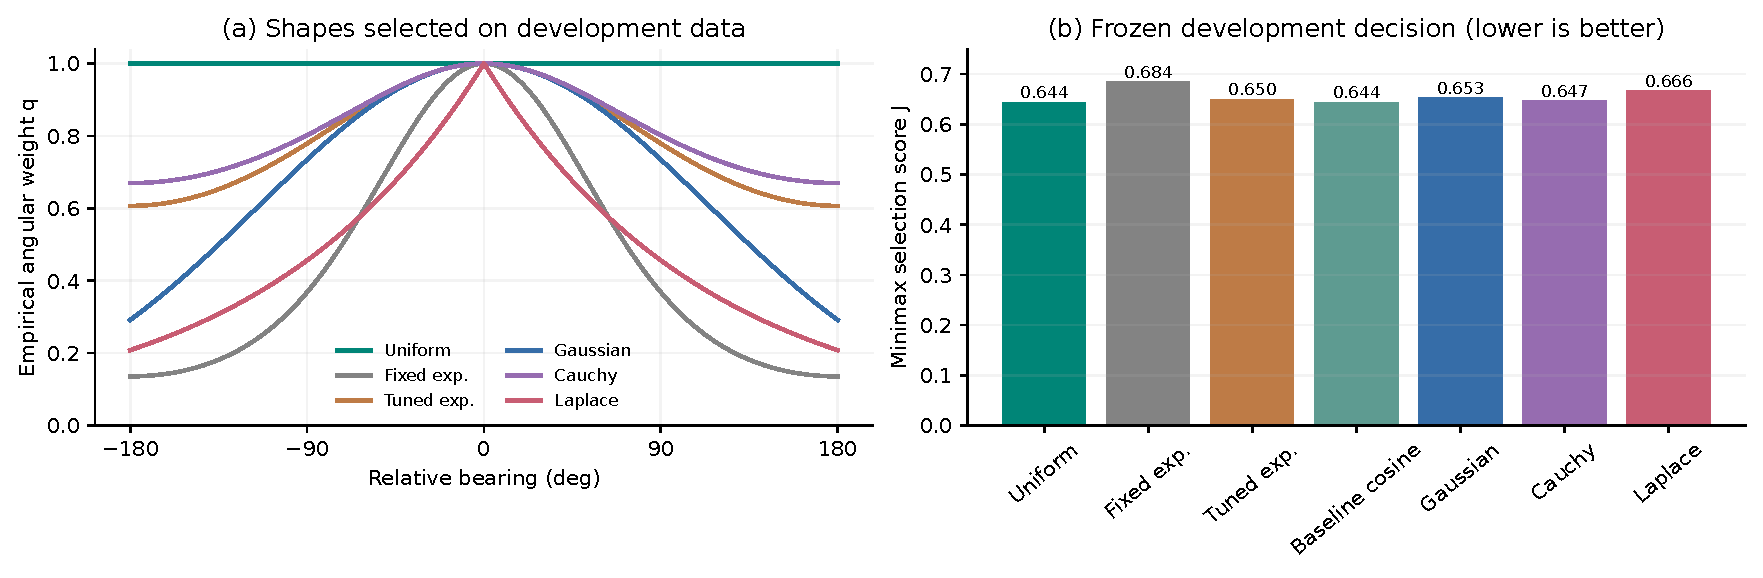
\includegraphics[width=\linewidth]{fig01_empirical_selection.pdf}
\caption{经验公式的开发选型。（a）各族选定的角度权重，余弦零参数与无衰减形式（Uniform）重合；（b）选择集评分 $J$，越小越好。}
\label{fig:empirical_selection}
\end{figure}
\begin{table}[!htbp]
\centering\small
\caption{候选经验公式的开发选型与独立测试。速度、活动为末20步平均响应预测 RMSE；场误差是另行拟合的输入场相对 RMSE。无衰减与余弦零参数为同式。}
\label{tab:empirical_results}
\begin{tabular}{lccccc}
\toprule
形式 & 选定参数 & 选择评分 $J$ & 速度 RMSE & 活动 RMSE & 场 RMSE\\
\midrule
无额外角度衰减 & -- & $0.64408$ & $0.122661$ & $0.011816$ & $0.379244$\\
固定指数 & $1$ & $0.68428$ & $0.125627$ & $0.012330$ & $0.220392$\\
可调指数 & $0.25$ & $0.64989$ & $0.124299$ & $0.011852$ & $0.227377$\\
带基线余弦 & $0$ & $0.64408$ & $0.122661$ & $0.011816$ & $0.379244$\\
圆周高斯 & $2$ & $0.65278$ & $0.121113$ & $0.011846$ & $0.191743$\\
环绕 Cauchy & $0.1$ & $0.64677$ & $0.124968$ & $0.011842$ & $0.385095$\\
圆周 Laplace & $2$ & $0.66641$ & $0.125963$ & $0.012207$ & $0.231627$\\
\bottomrule
\end{tabular}
\end{table}


\FloatBarrier
\subsubsection{独立测试结果}
图~\ref{fig:empirical_test}与表~\ref{tab:empirical_results}显示，所选公式的速度与活动 RMSE 分别为 $0.122661$、$0.011816$，较固定指数降低 $2.36\%$、$4.17\%$。速度 MSE 配对差为 $-0.0007363$，$95\%$ 区间为 $[-0.0010710,-0.0004016]$；活动差为 $-1.2408\times10^{-5}$，区间为 $[-1.6620,-0.8420]\times10^{-5}$。两项区间均低于零，满足预定的双指标改善判据。

宽高斯的速度 RMSE 比所选公式低 $1.26\%$，其速度 MSE 差区间为 $[-0.0005962,-0.0001587]$；活动差区间为 $[-1.4296,2.8674]\times10^{-6}$，跨零。场重建 RMSE 中，高斯为 $0.191743$，所选公式为 $0.379244$，固定指数为 $0.220392$。因此，$q=1$ 在所比较候选中的开发评分最低，高斯的速度与场重建误差更低。全部候选的速率 RMSE 为 $0.08525$--$0.08528$，差异较小。

\begin{figure}[!htbp]
\centering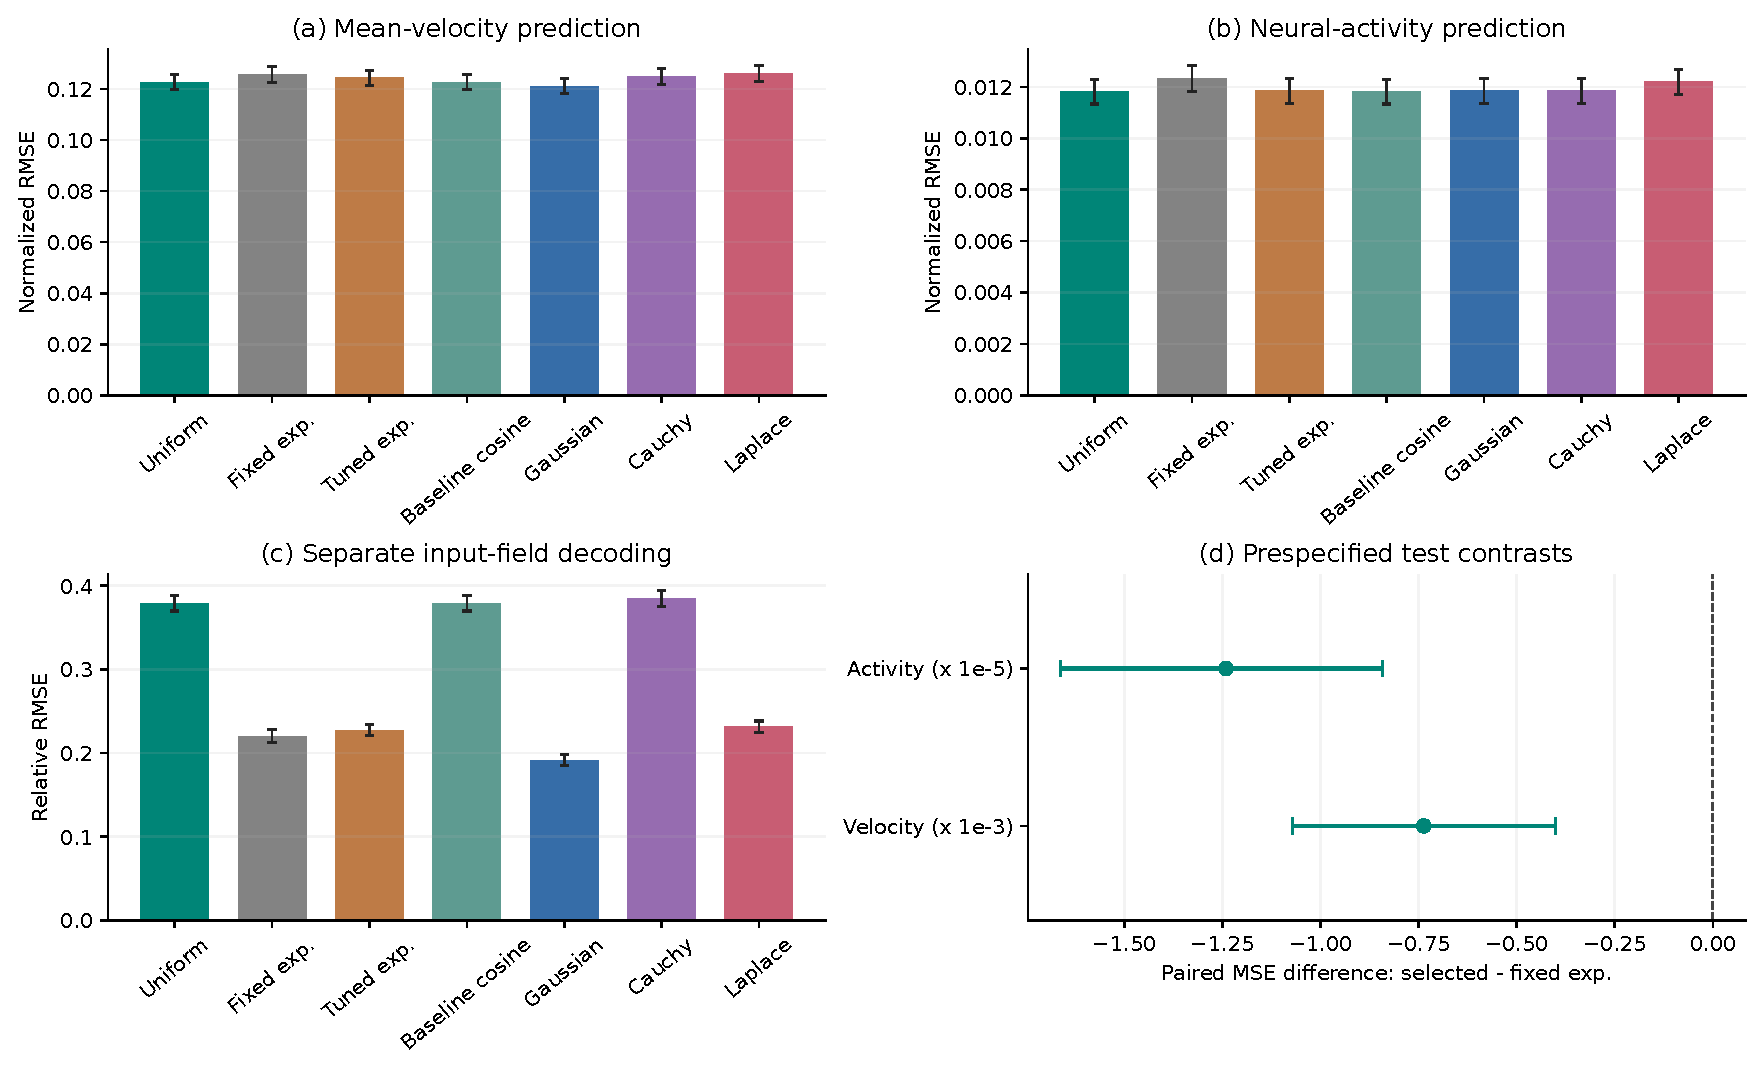
\includegraphics[width=\linewidth]{fig02_empirical_test.pdf}
\caption{独立测试的公式比较，$400$ 组几何、$9600$ 个条件。（a,b）末段平均速度与活动预测误差；（c）独立拟合的输入场解码误差；（d）预选 Uniform 相对固定指数的两项配对 MSE 差，横轴分别以 $10^{-3}$ 和 $10^{-5}$ 缩放。误差棒为 $95\%$ 几何 bootstrap 区间。}
\label{fig:empirical_test}
\end{figure}


图~\ref{fig:empirical_geometry}进一步比较各类几何。无衰减形式在聚集条件中的速度误差较小，宽高斯在均匀和前后双峰条件中更好。数量、强度与权重分层结果保存在数据目录；方向表示及初态变化的补充检验见附录~\ref{app:structure_experiment}。

\begin{figure}[!htbp]
\centering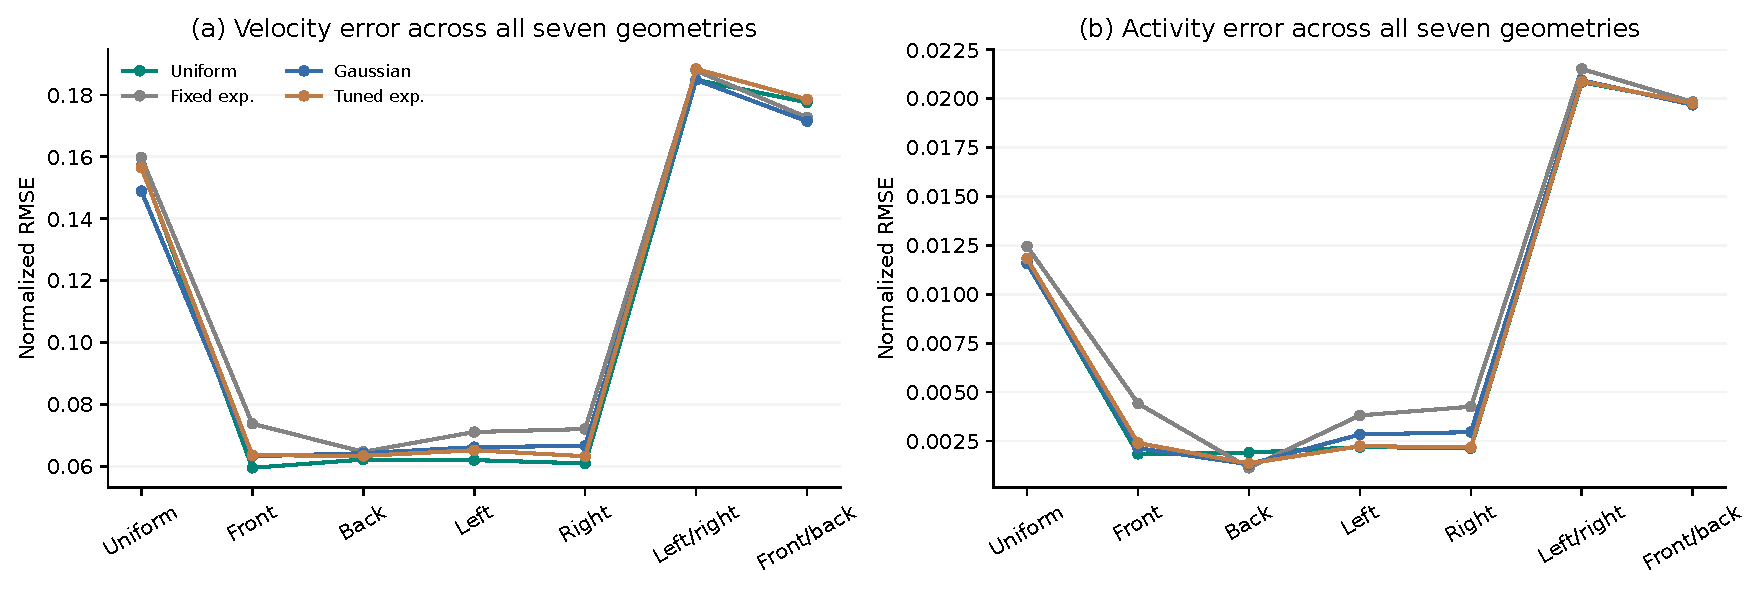
\includegraphics[width=\linewidth]{fig03_empirical_geometry.pdf}
\caption{七类结构中的经验公式预测误差。均匀结构 $160$ 个独立几何，其余各 $40$ 个，每组 $24$ 个条件；汇总评分按七类等权。曲线连接各类误差均值。}
\label{fig:empirical_geometry}
\end{figure}



\FloatBarrier

\subsubsection{社会输入机制的基准影响}

图~\ref{fig:input_mechanism} 同时给出输入幅值、角度覆盖、输入集中度、GO、LO 和凝聚距离。随机选邻并采用模型原定单邻居幅值时，增加 $n_e$ 会同时提高输入幅值和方向采样密度，使 GO、LO 上升并减小凝聚距离。固定总幅值后，输入幅值基本保持不变，但角度覆盖和输入集中度仍随选邻策略变化，反映了方向采样的作用。该结果支持将输入幅值和方位结构作为两个相互耦合且可区分的因素，并分别评价其对群体运动的影响。

\begin{figure}[!tbp]
 \centering
 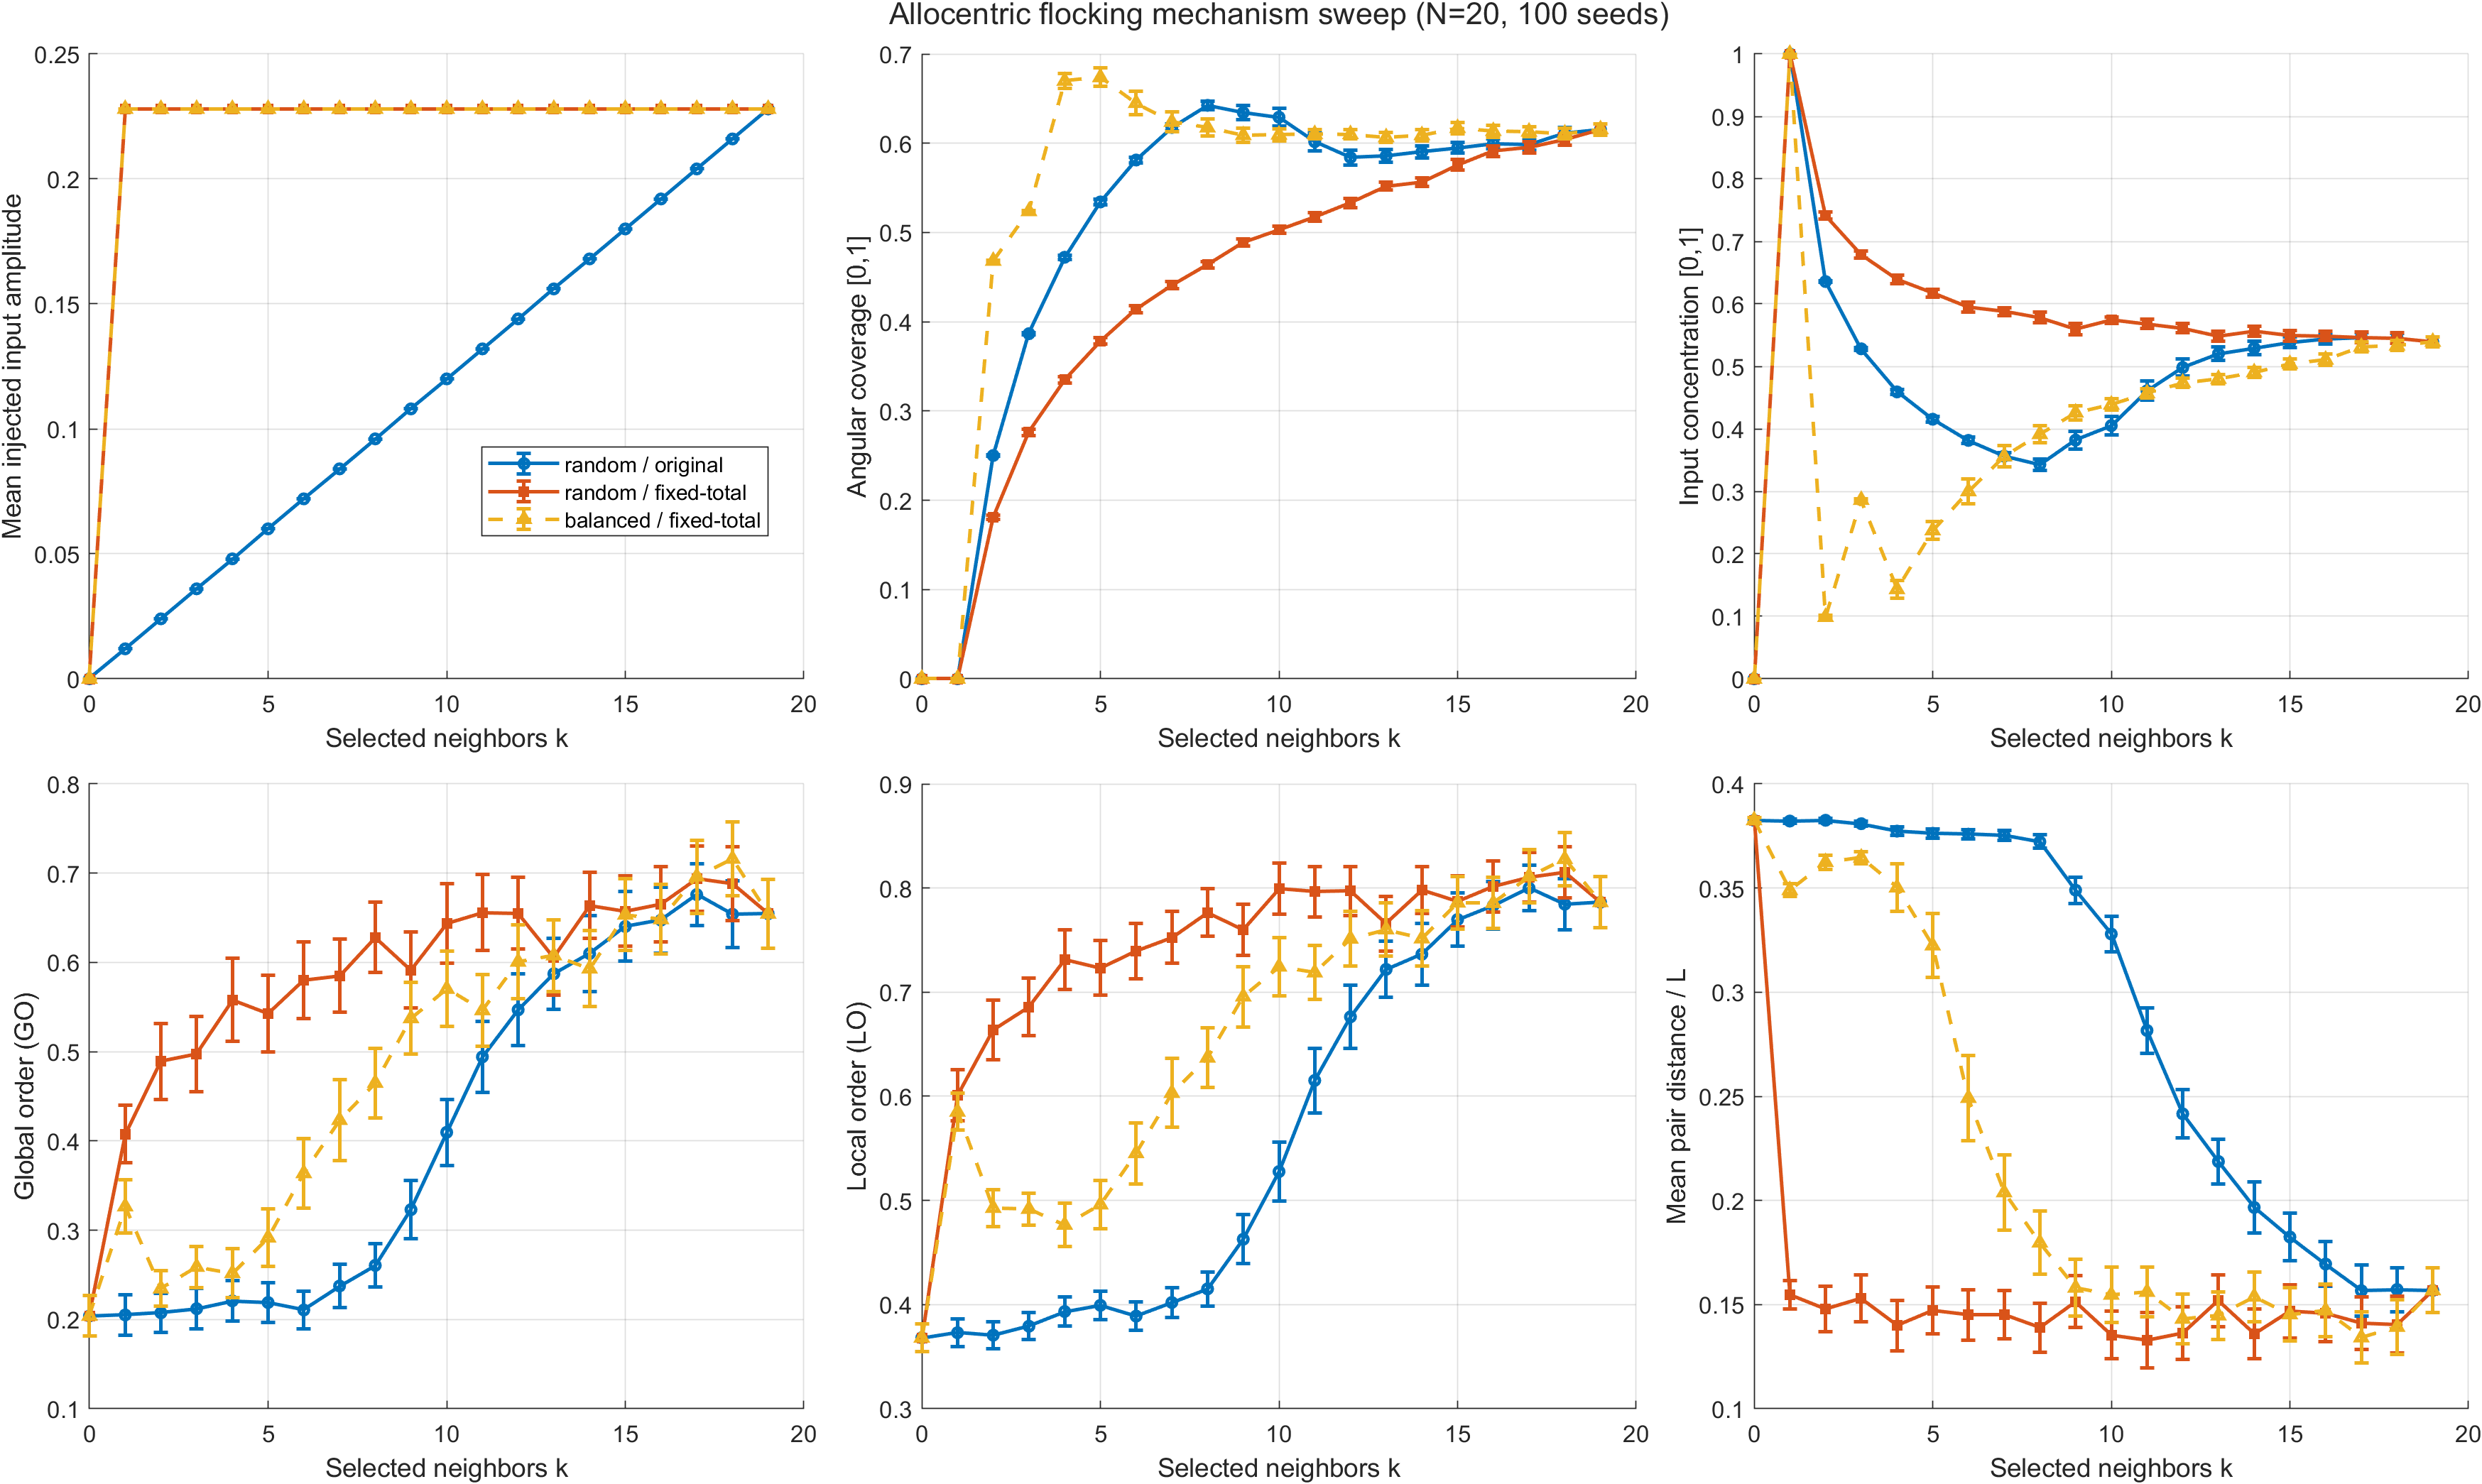
\includegraphics[width=0.96\linewidth]{fig1_input_mechanism.png}
 \caption{邻居数量、输入幅值和方位选择策略的机制分解（N=20，种子 1--100）。}
 \label{fig:input_mechanism}
\end{figure}


\subsection{挑战2：缺失方位预测与输入重建}\label{sec:challenge2_results}

本组实验沿“历史观测--方位后验--神经场输入”组织验证。方位预测评价方向随缺失时间的外推，协方差校准评价误差与不确定性的匹配，同状态回放评价预测信息经过周期核后的输入重建。本节先报告已有方位与输入诊断，随后给出基于共同样本的分层验证方案。

\subsubsection{已有结果：连续缺失下的协方差与方位预测}

连续缺失期间，常角速度模型的方位方差满足
\begin{equation}
 V(T)=p_{11}+2Tp_{12}+T^2p_{22}+q_\omega T^3/3
\end{equation}
其中短期单调性取决于交叉协方差。周期卷积使第 $n$ 阶方向谐波衰减为原来的 $\exp(-n^2V/2)$，方向核随方差增长而展宽，同时保持零阶输入。图~\ref{fig:uncertainty_diagnostics} 的上排给出解析性质，下排给出离线误差与 $95\%$ 区间经验覆盖率。较长遮挡下的低覆盖率反映了方位方差对实际误差的低估。闭环输入还受方差门控影响，其响应由方向核与激活边集合共同决定。

\begin{figure}[!tbp]
 \centering
 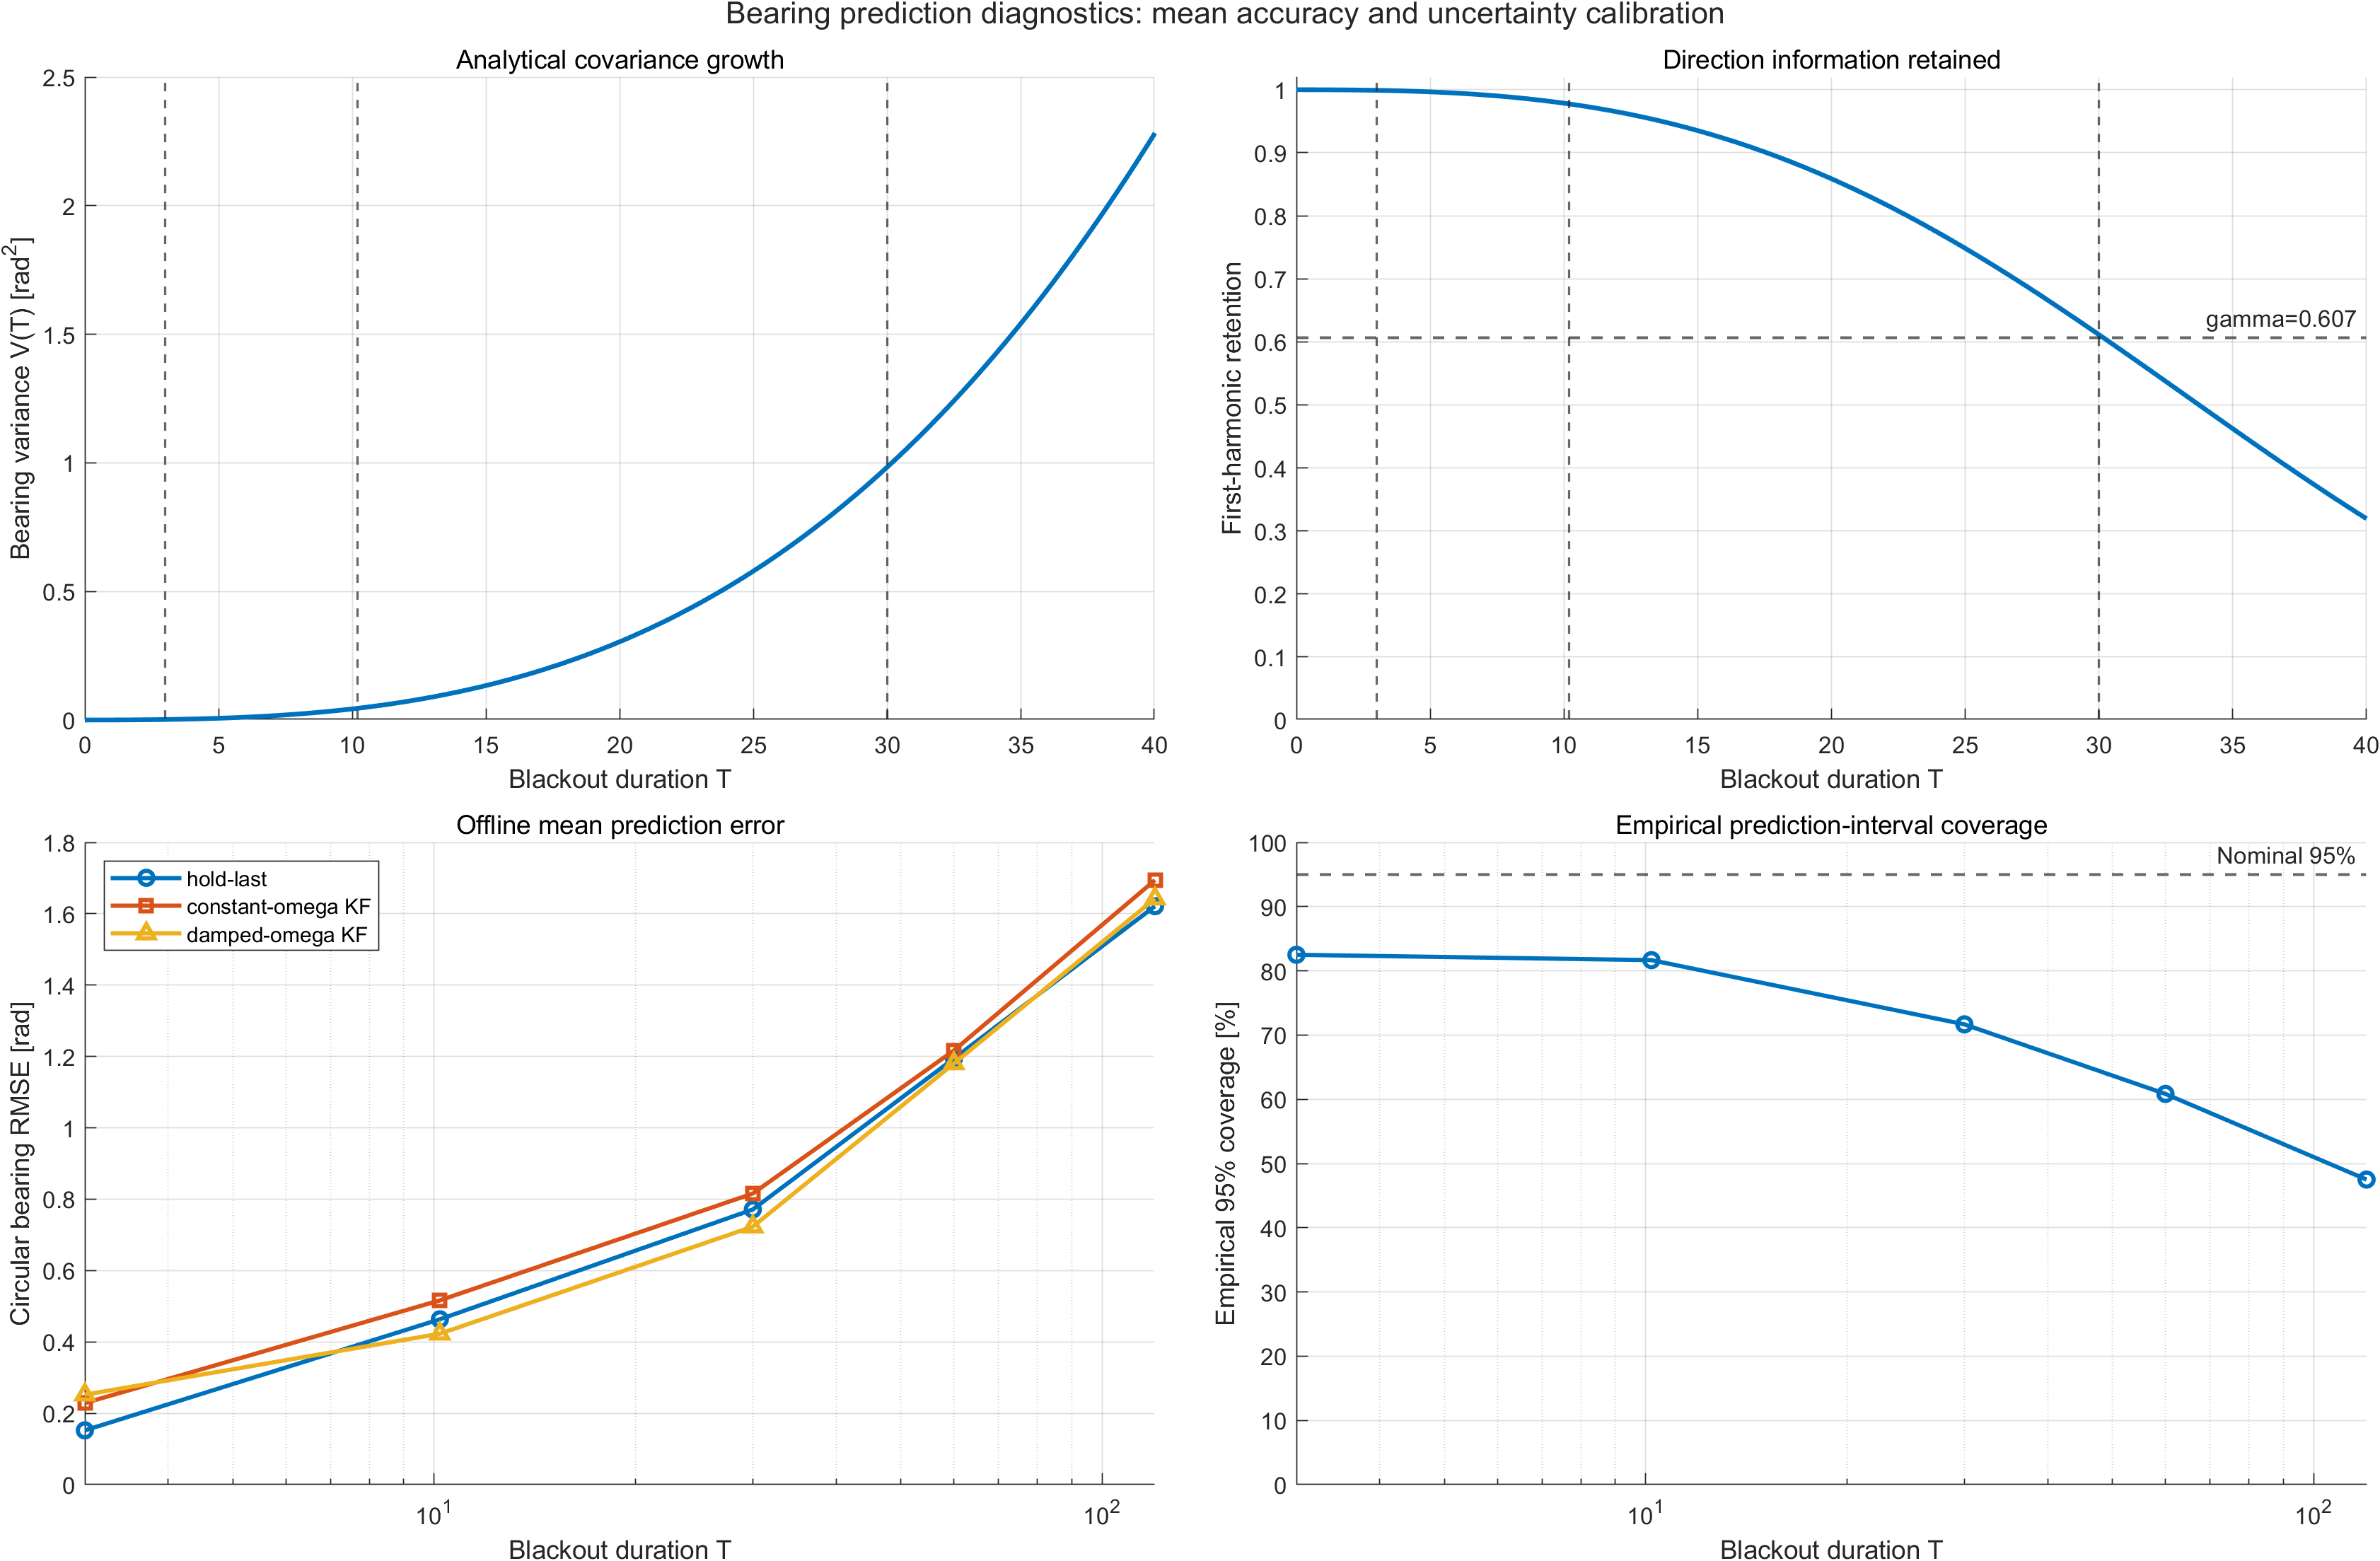
\includegraphics[width=0.98\linewidth]{kf-uncertainty-diagnostics.png}
 \caption{方位预测诊断。上排为解析协方差与方向信息保持；下排为离线均值误差和 95\% 经验覆盖率（种子 138--141）。}
 \label{fig:uncertainty_diagnostics}
\end{figure}

图~\ref{fig:predict_error} 给出隐藏且激活边的平均绝对圆周误差。相较 hold-last，KF-GM 在 $6\le T\le30$ 时误差降低约 $13\%$--$19\%$，在 $T=60$ 时降低约 $9\%$--$10\%$，相应配对 bootstrap 区间均不跨零。$T=3$ 时均值降低约 $11\%$--$13\%$，其中两种较强遮挡条件的区间跨零。误差按缺失且仍激活的边累计：$T=60$ 包含 $200$ 步，常角速度 KF 受方差门限约束，其有效窗口为前 $100$ 步，hold 与 GM 为全部 $200$ 步。隐藏 $11$ 边时，每种子的有效边--时间点分别为 $22000$ 和 $44000$，因此图中省略常角速度 KF 的 $T=60$ 点。闭环 GO 与距离按完整窗口统计，评价预测与门控的组合响应。

\begin{figure}[!tbp]
 \centering
 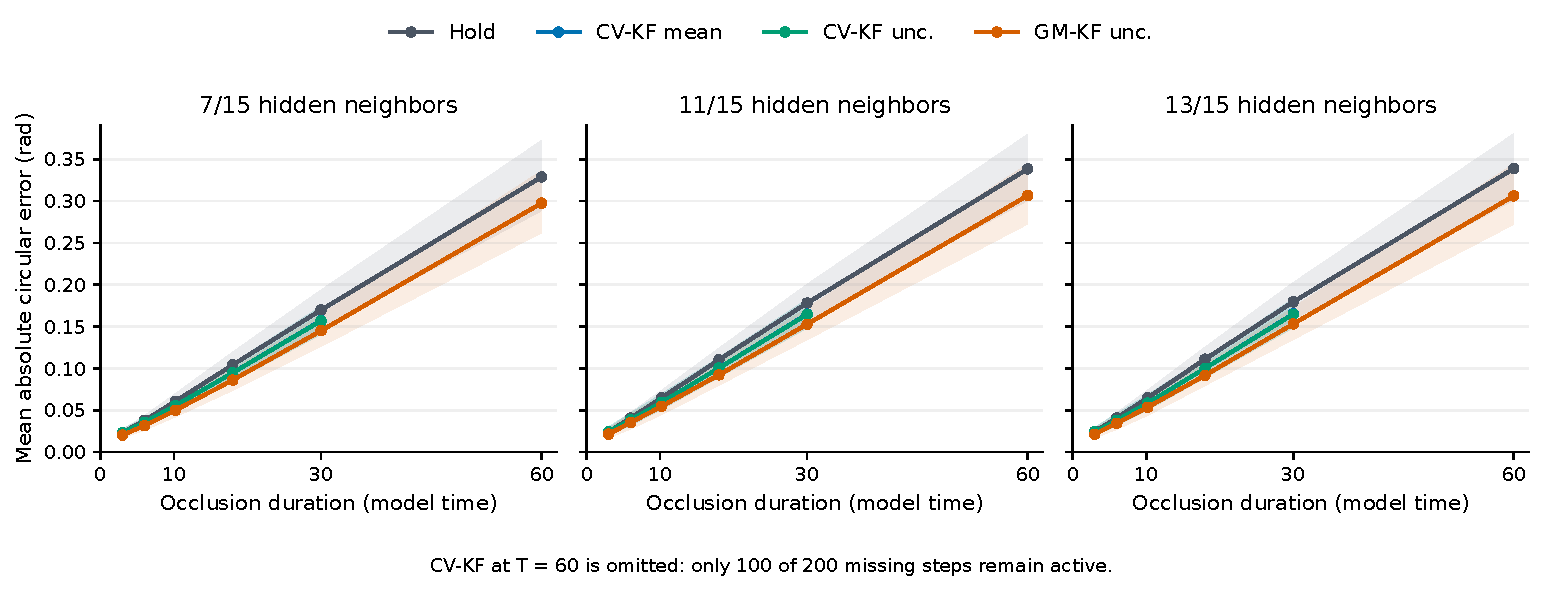
\includegraphics[width=\linewidth]{kf-prediction-error-v4.pdf}
 \caption{扩展批次隐藏且激活边的平均绝对圆周误差。共 $30$ 个种子，阴影为逐条件 $95\%$ 配对 bootstrap 区间。常角速度 KF 在 $T=60$ 时的有效窗口为前 $100/200$ 步，图中省略该点；hold 与 GM 使用完整窗口。方位真值用于离线误差计算。}
 \label{fig:predict_error}
\end{figure}


\subsubsection{已有结果：五种子方位与输入重建诊断}
\label{sec:kf_pilot}

本组以五个开发种子 $1$--$5$ 组织方位预测、同状态输入回放和检查点分叉。方位与输入重建诊断在本节报告，共用数据的群体响应在第~\ref{sec:challenge3_results} 节展开，形成从方向预测到群体运动的连续评价。

\paragraph{实验条件与对照方法}

每个智能体固定选择编号向后的 $8$ 个循环邻居，等权输入，总权重记为 $A_0$。完整观测运行至第 $6200$ 步，在最后合法观测上冻结隐藏邻居身份；第 $6201$--$6234$ 步屏蔽方位，共 $34$ 步，即 $10.2$ 个模型时间单位，第 $6235$ 步恢复，仿真运行至第 $6600$ 步。观测无噪声，方位采用世界坐标系，输入强度保持最后合法值。KF 采用常角速度状态，$q_\omega=10^{-6}$、$R=10^{-4}$、$P_0=\operatorname{diag}(R,1)$，初始角速度为零。此处 $R$ 为固定的假定观测方差与数值正则量；协方差通过覆盖率和恢复首步 NIS 诊断。

围绕中心条件 $h=4$、random、$A_0=0.228$，分别扫描隐藏邻居数 $h\in\{2,4,6\}$、隐藏方位结构 random/concentrated/dispersed，以及 $A_0\in\{0.114,0.228,0.456\}$，共 $7$ 个唯一条件。concentrated 和 dispersed 在最后合法观测上分别选择一阶圆周合矢量模 $R_1^{\mathcal H}=|h^{-1}\sum_{j\in\mathcal H_i}e^{\mathrm{i}\theta_{ij}}|$ 最大和最小的隐藏集合。每个 $A_0$ 均重新运行完整前缀，同一 $(\text{seed},A_0)$ 内各方法共享检查点；幅值扫描因而同时包含预热动力学的变化。

对照包括：fresh 始终使用完整当前观测；drop 删除缺失边；drop-normalized 将可见边权重调整为 $A_0/(8-h)$，保持总幅值；hold 保持缺失边的最后方位及权重；KF-mean 按式~\eqref{eq:pilot_causal_input} 注入预测均值。drop 对应幅值与方位同时减少，drop-normalized 保留幅值而减少方位覆盖，hold 延续历史方位，KF-mean 在相同缓存权重上增加方向外推。恢复首步各方法均使用当前合法观测。新批次评估均值外推及协方差诊断，协方差卷积的闭环结果在后续扩展时长实验中分别报告。

每个种子有 $3$ 条 fresh 参考轨迹和 $7\times4=28$ 条非 fresh 轨迹，五个种子共 $155$ 条唯一闭环轨迹；同一 fresh 轨迹在对应条件中重复引用。另有 $35$ 组同状态输入回放，以及 $7\times5\times3=105$ 项离线 $R$ 诊断，其中替代 $R=10^{-6},10^{-2}$ 均使用相同的完整 $6200$ 步合法历史。统计按种子配对，采用 $5000$ 次种子组 bootstrap，随机种子为 $20261010$，所有条件共用重采样索引。

\paragraph{评价指标与解释}

离线层在 fresh 轨迹上屏蔽固定邻居观测，以缺失期间全部隐藏边--时间点的圆周误差计算每个种子的方位 RMSE，再对五个种子取均值。覆盖率为 $|e_{ij}|\le1.96\sqrt{P_{11,ij}^{-}}$ 的边--时间点比例；归一化创新平方（NIS）为恢复首步的 $\nu_{ij}^2/(P_{11,ij}^{-}+R)$，在隐藏边上取均值，用于比较预测创新与假定方差。同状态层让各候选输入读取相同 fresh 状态，比较完整神经场输入向量，定义
\begin{equation}
 E_I^{(s)}=\frac{1}{N|\mathcal K_o|}
 \sum_{k\in\mathcal K_o}\sum_{i=1}^N
 \frac{\|I_i^{(s)}(k)-I_i^{\mathrm{fresh}}(k)\|_2}
 {\|I_i^{\mathrm{fresh}}(k)\|_2}.
 \label{eq:pilot_input_error}
\end{equation}
该误差直接描述在相同几何状态下输入场的重建程度；第~\ref{sec:social_input_model} 节的 $S_i$ 则描述方位加权后的标量输入量。

\paragraph{方位预测及协方差诊断结果}

中心条件下，KF-mean 的逐种子 RMSE 均值为 $0.1040$ rad，hold 为 $0.1414$ rad，降低 $26.4\%$，五个种子中四个误差更低。种子 $2$ 的 KF 误差为 $0.3757$ rad，高于 hold 的 $0.2348$ rad，体现了常角速度外推对具体轨迹的敏感性。图~\ref{fig:kf_pilot_prediction}a--c 中，隐藏数量从 $2$ 增至 $6$ 时，KF 均值误差从 $0.1012$ 增至 $0.1148$ rad；集中与分散结构下分别为 $0.0976$ 和 $0.1396$ rad。低幅值 $A_0=0.114$ 时 KF 为 $0.2229$ rad，高于 hold 的 $0.2002$ rad；$A_0=0.456$ 时 KF 降至 $0.000481$ rad。这些变化反映了不同输入条件及其预热轨迹下的预测表现。

\paragraph{逐种子与合并误差}
中心条件各个种子均有 $2720=20\times4\times34$ 个隐藏边--时间点。设第 $r$ 个种子的 RMSE 为 $r_r$，逐种子均值为 $5^{-1}\sum r_r$，合并 RMSE 为 $\sqrt{5^{-1}\sum r_r^2}$，重采样单位均为种子。表~\ref{tab:rmse_sensitivity} 显示，KF 在 $4/5$ 个种子中误差更低，而种子 $2$ 的较大误差使合并 RMSE 比 hold 增高 $13.5\%$。逐种子 RMSE 差值（KF 减 hold）为 $-0.03739$ rad，$95\%$ 配对 bootstrap 区间为 $[-0.11198,0.06002]$，包含零。两种汇总的差异表明，方位预测误差具有明显的种子异质性，合并 RMSE 对较大误差更为敏感。

\begin{table}[!tbp]
\centering\small
\caption{中心条件下五个种子的方位 RMSE、逐种子均值与合并 RMSE（rad）。}
\label{tab:rmse_sensitivity}
\begin{tabular}{lrr}
\toprule 种子或汇总方式 & hold & KF-mean\\\midrule
1 & 0.150014 & 0.000677\\
2 & 0.234778 & 0.375660\\
3 & 0.095930 & 0.039982\\
4 & 0.162777 & 0.091770\\
5 & 0.063641 & 0.012095\\\midrule
逐种子 RMSE 均值 & 0.141428 & 0.104037\\
合并平方误差后开根号 & 0.153215 & 0.173947\\\bottomrule
\end{tabular}
\end{table}

主 $R$ 下，中心条件名义 $95\%$ 区间的经验覆盖率为 $89.76\%$，种子范围为 $65.74\%$--$100\%$，恢复首步平均 NIS 为 $76.45$。图~\ref{fig:kf_pilot_prediction}d 展示不同假定 $R$ 下的覆盖率；种子 $2$ 的低覆盖率与较大预测误差相对应，反映了当前运动模型和方差设定的失配。

\begin{figure}[!tbp]
 \centering
 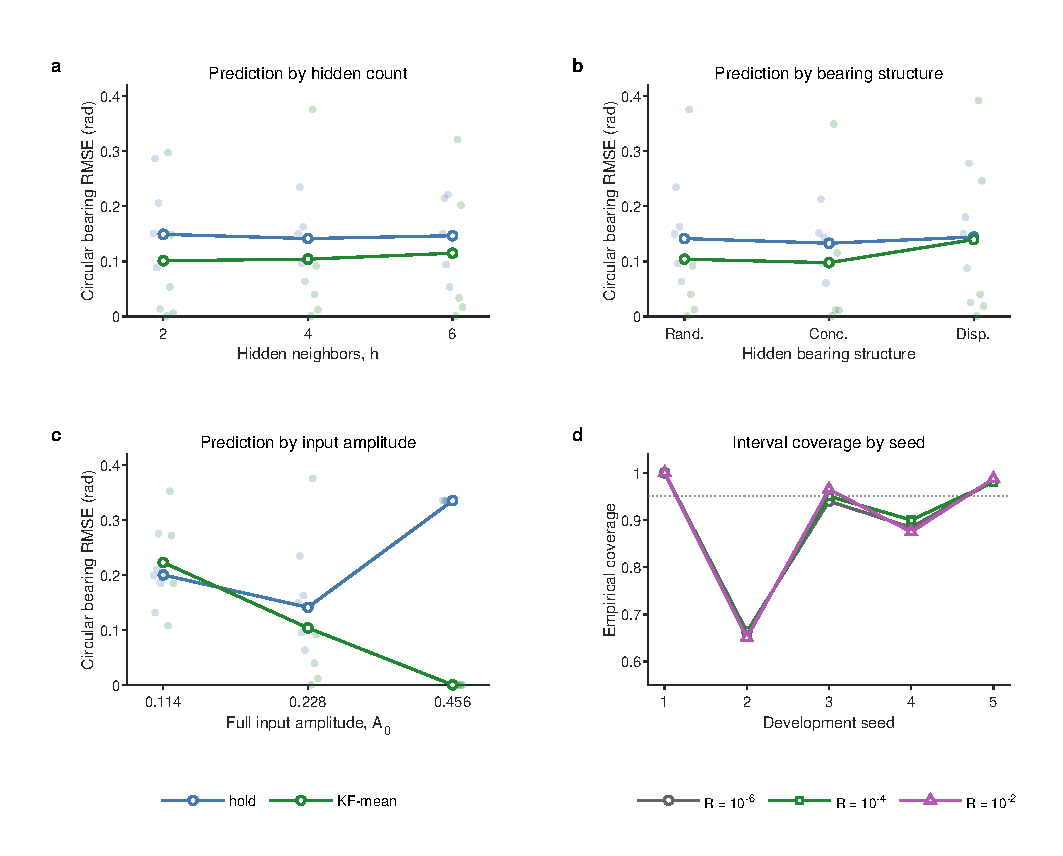
\includegraphics[width=\linewidth]{fig04_kf_prediction.pdf}
 \caption{五种子开发实验中的方位预测与覆盖率诊断。（a--c）分别扫描隐藏邻居数、隐藏方位结构和完整观测总幅值；连线点为五个逐种子圆周 RMSE 的均值，浅色散点为各种子值，主 $R=10^{-4}$。三个扫描共享中心条件 $h=4$、random、$A_0=0.228$。（d）中心条件下三个假定 $R$ 的逐种子经验覆盖率，虚线为名义 $0.95$。全部条件的连续缺失时长为 $34$ 步、$10.2$ 个模型时间单位；重采样单位为 $5$ 个开发种子。}
 \label{fig:kf_pilot_prediction}
\end{figure}


\paragraph{同状态输入重建结果}
表~\ref{tab:kf_pilot_center} 中，中心条件的同状态输入误差从 drop 的 $0.5143$ 降至 drop-normalized 的 $0.2671$，说明恢复总幅值补偿了部分输入差异。hold 和 KF-mean 的误差分别为 $0.05507$ 和 $0.02103$，后者相对降低 $61.8\%$。五个种子的配对误差差值（KF 减 hold）为 $-0.03404$，$95\%$ bootstrap 区间为 $[-0.06738,-0.00790]$。两者采用相同缓存权重，方向外推在保留历史方位的基础上进一步降低了同状态方向场的重建误差。


\subsubsection{后续实验：共同样本下的分层验证}\label{sec:challenge2_plan}
分层实验将使用相同的完整观测前缀、缺失边集合和观测噪声，在同一参考几何上回放删除输入、幅值归一化、方位保持、均值预测和协方差卷积。场景包括直行参考、方向变化和自主相互转向；在每类场景中分别改变隐藏数量、方位集中度、输入强度及缺失时长。参数选择和独立评估采用互不重叠的种子，以逐种子配对差及区间汇总各项响应。

方位层将同时报告圆周 RMSE、绝对角误差、经验覆盖率和恢复首步 NIS。比较采用共同隐藏边与共同时间窗；对门控后停止注入的边，继续保存预测诊断，从而将方位模型的外推误差与门控选择的作用分别呈现。运动模型、过程噪声和方差参数在开发样本中确定，冻结后进入独立评估。

输入层将比较完整周期输入场的相对误差、积分强度和方向谐波，并同步记录神经活动及二维速度。均值/协方差输入、运动模型和门控配置采用逐项对照，建立各组件对输入重建的作用关系。最终形成分场景、分时长的方位精度、协方差校准和输入误差结果，作为挑战3选择预测配置与扫描区间的依据。



\begin{table}[!htbp]
\centering\small
\caption{挑战2后续分层验证的对照与输出设计}
\label{tab:layered_validation_plan}
\begin{tabular}{>{\raggedright\arraybackslash}p{0.14\linewidth}
                >{\raggedright\arraybackslash}p{0.34\linewidth}
                >{\raggedright\arraybackslash}p{0.42\linewidth}}
\toprule
评价层次 & 共同样本下的对照 & 拟记录的主要输出\\
\midrule
方位外推 & 方位保持、常角速度与阻尼角速度模型 & 圆周误差、完整隐藏边数、预测时长、覆盖率、恢复首步 NIS\\[3pt]
输入重建 & 删除、幅值归一化、方位保持、均值核与协方差核 & 完整场误差、积分强度、方向谐波、神经活动与二维速度\\[3pt]
组件作用 & 固定其余配置，逐项比较运动模型、卷积与门控 & 逐种子配对差、实际激活边、共同时间窗及门控后的诊断\\
\bottomrule
\end{tabular}
\end{table}
分层实验将先固定数据划分、评价窗口和对照配置，再按场景给出分时长误差与区间，并汇总各类场景的综合表现。最终输出包括冻结的重建配置、场景分层结果和逐种子记录，供第~\ref{sec:challenge3_plan} 节的边界实验使用。


\subsection{挑战3：群体闭环响应与条件边界}\label{sec:challenge3_results}

本组实验对应第~\ref{sec:group_method} 节的群体评价框架。扩展遮挡实验比较无外部转向干预时的补偿响应，受控转向实验评价方向变化过程中的群体协调；边界实验将以挑战2确定的预测重建配置为基础，进一步研究新鲜输入数量、方位结构与缺失时长的联合影响。


\subsubsection{已有结果：输入重建与群体响应的联动}

本组沿用第~\ref{sec:kf_pilot} 节的五种子开发数据，将同状态输入误差与各自分叉后的群体响应并列报告。表~\ref{tab:kf_pilot_center}及图~\ref{fig:kf_pilot_input_response}连接输入重建与凝聚结构的变化。

闭环层在共同检查点上分别推进，主响应为恢复后 $100$ 步，即 $\mathcal K_r=\{6235,\ldots,6334\}$ 内的有符号平均对距变化
\begin{equation}
 \Delta D^{(s)}=\frac{1}{|\mathcal K_r|}\sum_{k\in\mathcal K_r}
 \frac{d^{(s)}(k)-d^{\mathrm{fresh}}(k)}{L},
 \quad
 D_{\mathrm{abs}}^{(s)}=\frac{1}{|\mathcal K_r|}\sum_{k\in\mathcal K_r}
 \frac{|d^{(s)}(k)-d^{\mathrm{fresh}}(k)|}{L},
 \label{eq:pilot_distance_metrics}
\end{equation}
其中 $d$ 为周期最短两两距离均值。$\Delta D$ 的正、负值分别表示相对 fresh 更分散、更紧凑，$D_{\mathrm{abs}}$ 补充描述偏离大小。GO 和 LO 的损失定义为相同窗口内 fresh 减去候选分支的时间平均值。


\begin{table}[!tbp]
 \centering
 \small
 \caption{中心条件下五个种子的平均响应。$h=4$、random、$A_0=0.228$；输入误差在同一 fresh 状态上计算，距离与 GO 在闭环恢复后 $100$ 步计算。距离列及 GO 损失列按表头缩放；$\Delta D$ 为有符号变化，$D_{\mathrm{abs}}$ 为逐时刻绝对偏离的平均值。}
 \label{tab:kf_pilot_center}
 \begin{tabular}{lrrrr}
  \toprule
  方法 & $E_I$ & $10^3\Delta D$ & $10^3D_{\mathrm{abs}}$ & $10^3$ GO 损失\\
  \midrule
  fresh & $0$ & $0$ & $0$ & $0$\\
  drop & $0.51426$ & $1.60580$ & $1.60580$ & $-7.09418$\\
  drop-normalized & $0.26710$ & $0.07157$ & $0.32839$ & $-2.16612$\\
  hold & $0.05507$ & $0.58979$ & $0.58979$ & $-1.86953$\\
  KF-mean & $0.02103$ & $0.08120$ & $0.08181$ & $-1.34723$\\
  \bottomrule
 \end{tabular}
\end{table}

闭环层的响应体现了输入重建与群体指标之间的非线性联系。中心条件下，KF-mean 的 $\Delta D=8.12\times10^{-5}$，hold 为 $5.90\times10^{-4}$；drop-normalized 的有符号均值略低于 KF，但其绝对偏离为 $3.28\times10^{-4}$，高于 KF 的 $8.18\times10^{-5}$，说明符号抵消会影响单纯均值比较。四种非 fresh 分支的中心条件 GO 损失均为负，即该窗口内 GO 略高于 fresh，同时仍存在距离结构偏移，体现了有序度与凝聚响应的不同侧面。

图~\ref{fig:kf_pilot_input_response}a--c 显示，增加隐藏数量使输入场重建误差上升；在七个条件中 KF-mean 的平均输入误差均低于 hold。图~\ref{fig:kf_pilot_input_response}d--f 的对距变化则具有非单调性：数量扫描中 KF 的有符号变化为 $6.51\times10^{-5}$、$8.12\times10^{-5}$、$2.74\times10^{-5}$；分散结构及高幅值条件的均值略为负。在 $35$ 个种子--条件配对中，KF 相对 hold 的有符号变化和绝对偏离分别在 $34$ 项中更低，各项共享同一批五个种子。结果支持将方位预测、输入场重建和闭环响应逐层评价：预测提供的方向信息改善了输入重建，群体指标还受神经场非线性与分叉轨迹影响。

\begin{figure}[!tbp]
 \centering
 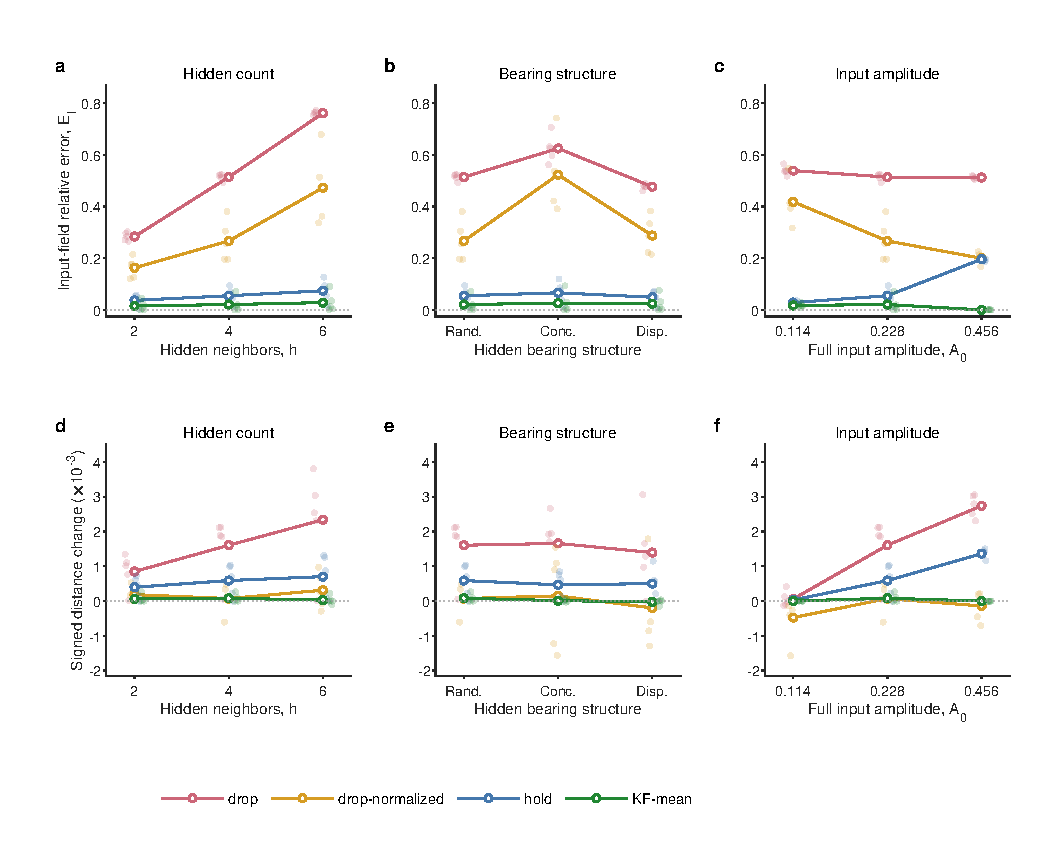
\includegraphics[width=\linewidth]{fig05_kf_input_response.pdf}
 \caption{输入重建与闭环对距响应的三条单因素扫描。（a--c）缺失期间在同一 fresh 状态上计算的完整输入场相对误差 $E_I$；（d--f）恢复后 $100$ 步的有符号对距变化 $\Delta D$，纵轴单位为 $10^{-3}$。各列分别改变隐藏数量、方位结构和完整观测总幅值，中心条件与图~\ref{fig:kf_pilot_prediction} 一致。连线点为五种子均值，浅色散点为逐种子值；零线对应 fresh 参考。负值表示相对 fresh 更紧凑，连线用于辨识三个离散水平。}
 \label{fig:kf_pilot_input_response}
\end{figure}




\subsubsection{已有结果：扩展遮挡时长下的闭环补偿}

为量化补偿分支对无遮挡参考行为的再现程度，采用 GO 的绝对偏差作为主响应。记 $\mathcal K_o$ 为连续遮挡时间步集合，定义
\begin{equation}
 D_{\mathrm{GO}}=\frac{1}{|\mathcal K_o|}\sum_{k\in\mathcal K_o}
 \left|GO_{\mathrm{control}}(k)-GO_{\mathrm{method}}(k)\right|,
\end{equation}
遮挡后凝聚距离偏差采用相同定义。对于逐种子偏差 $D_{r,s}$，相对 fresh-drop 的降低比例为 $1-\overline D_s/\overline D_{\mathrm{drop}}$。区间按种子配对重采样 $5000$ 次得到，Python 随机数基础种子为 $20260915$，并使用条件偏移。各条件复用相同的 $30$ 个种子；所报区间为未作多重比较校正的逐条件探索性区间，偏差降低表示候选轨迹更接近无遮挡参考。

表~\ref{tab:kf_go} 和表~\ref{tab:kf_pair} 给出隐藏 $11/15$ 条输入时 GO 偏差与遮挡后距离偏差相对 fresh-drop 的降低比例。hold-last 描述保留历史方位的响应，Kalman 与 hold 的配对差值评价方向外推及协方差输入的增量。各单元格报告点估计与逐条件 $95\%$ bootstrap 区间。

\begin{table}[!tbp]
 \centering
 \small
 \caption{隐藏 $11/15$ 条输入时 GO 偏差相对 fresh-drop 的降低比例}
 \label{tab:kf_go}
 \setlength{\tabcolsep}{5pt}
\begin{tabular}{lcccc}
\toprule
$T$ & hold & KF-mean & KF-unc & KF-GM\\
\midrule
3 & \shortstack{81.6\\[-1pt]{\scriptsize [72.6, 88.2]}} & \shortstack{86.4\\[-1pt]{\scriptsize [78.9, 91.3]}} & \shortstack{86.2\\[-1pt]{\scriptsize [78.9, 91.2]}} & \shortstack{86.5\\[-1pt]{\scriptsize [78.4, 92.4]}}\\[4pt]
6 & \shortstack{75.0\\[-1pt]{\scriptsize [64.6, 82.5]}} & \shortstack{82.3\\[-1pt]{\scriptsize [74.6, 87.7]}} & \shortstack{82.3\\[-1pt]{\scriptsize [74.8, 88.0]}} & \shortstack{83.3\\[-1pt]{\scriptsize [74.4, 89.2]}}\\[4pt]
10.2 & \shortstack{68.6\\[-1pt]{\scriptsize [55.8, 77.6]}} & \shortstack{77.9\\[-1pt]{\scriptsize [68.6, 84.4]}} & \shortstack{77.0\\[-1pt]{\scriptsize [67.0, 84.4]}} & \shortstack{79.5\\[-1pt]{\scriptsize [69.9, 86.0]}}\\[4pt]
18 & \shortstack{63.5\\[-1pt]{\scriptsize [50.2, 73.1]}} & \shortstack{71.5\\[-1pt]{\scriptsize [59.7, 79.9]}} & \shortstack{67.7\\[-1pt]{\scriptsize [53.0, 77.9]}} & \shortstack{72.7\\[-1pt]{\scriptsize [62.2, 80.2]}}\\[4pt]
30 & \shortstack{58.2\\[-1pt]{\scriptsize [43.9, 68.6]}} & \shortstack{63.1\\[-1pt]{\scriptsize [45.9, 74.7]}} & \shortstack{52.6\\[-1pt]{\scriptsize [31.4, 66.8]}} & \shortstack{62.6\\[-1pt]{\scriptsize [47.1, 73.4]}}\\[4pt]
60 & \shortstack{47.9\\[-1pt]{\scriptsize [30.9, 59.7]}} & \shortstack{46.9\\[-1pt]{\scriptsize [30.8, 59.7]}} & \shortstack{33.7\\[-1pt]{\scriptsize [13.3, 49.0]}} & \shortstack{46.4\\[-1pt]{\scriptsize [26.9, 60.4]}}\\[4pt]
\bottomrule
\end{tabular}
\par\smallskip\footnotesize 数值单位为百分比；方括号为逐条件 $95\%$ 配对 bootstrap 区间。
\end{table}

\begin{table}[!tbp]
 \centering
 \small
 \caption{隐藏 $11/15$ 条输入时遮挡后距离偏差相对 fresh-drop 的降低比例}
 \label{tab:kf_pair}
 \setlength{\tabcolsep}{5pt}
\begin{tabular}{lcccc}
\toprule
$T$ & hold & KF-mean & KF-unc & KF-GM\\
\midrule
3 & \shortstack{89.3\\[-1pt]{\scriptsize [83.0, 93.8]}} & \shortstack{89.7\\[-1pt]{\scriptsize [80.3, 95.0]}} & \shortstack{89.8\\[-1pt]{\scriptsize [81.0, 95.2]}} & \shortstack{91.3\\[-1pt]{\scriptsize [85.3, 95.3]}}\\[4pt]
6 & \shortstack{85.5\\[-1pt]{\scriptsize [80.3, 90.0]}} & \shortstack{89.7\\[-1pt]{\scriptsize [85.2, 93.2]}} & \shortstack{89.4\\[-1pt]{\scriptsize [84.9, 92.8]}} & \shortstack{91.2\\[-1pt]{\scriptsize [87.1, 94.6]}}\\[4pt]
10.2 & \shortstack{79.3\\[-1pt]{\scriptsize [71.7, 85.3]}} & \shortstack{89.0\\[-1pt]{\scriptsize [84.5, 92.8]}} & \shortstack{86.5\\[-1pt]{\scriptsize [80.0, 90.8]}} & \shortstack{87.0\\[-1pt]{\scriptsize [81.5, 91.6]}}\\[4pt]
18 & \shortstack{70.1\\[-1pt]{\scriptsize [59.5, 78.8]}} & \shortstack{88.1\\[-1pt]{\scriptsize [83.3, 91.8]}} & \shortstack{83.4\\[-1pt]{\scriptsize [73.4, 89.6]}} & \shortstack{80.1\\[-1pt]{\scriptsize [71.0, 87.2]}}\\[4pt]
30 & \shortstack{59.0\\[-1pt]{\scriptsize [46.8, 69.2]}} & \shortstack{85.6\\[-1pt]{\scriptsize [78.8, 90.6]}} & \shortstack{79.5\\[-1pt]{\scriptsize [67.7, 87.1]}} & \shortstack{71.5\\[-1pt]{\scriptsize [61.2, 79.8]}}\\[4pt]
60 & \shortstack{40.2\\[-1pt]{\scriptsize [29.7, 50.1]}} & \shortstack{59.0\\[-1pt]{\scriptsize [52.0, 65.8]}} & \shortstack{64.0\\[-1pt]{\scriptsize [55.8, 71.3]}} & \shortstack{55.3\\[-1pt]{\scriptsize [46.7, 63.4]}}\\[4pt]
\bottomrule
\end{tabular}
\par\smallskip\footnotesize 数值单位为百分比；方括号为逐条件 $95\%$ 配对 bootstrap 区间。
\end{table}

hold-last 在短中时遮挡中解释了大部分偏差降低。Kalman 相对 hold 的增量随指标和时间尺度变化：$T\le30$ 时，KF-mean 和 KF-GM 的 GO 偏差较低；$T=60$ 时，两者的均值略高。KF-uncertainty 在 $T=60$ 时的遮挡后距离偏差相对 fresh-drop 降低约 $64\%$，高于 hold-last 的 $40.2\%$。这些响应来自所比较模型、输入核及门控配置的整体作用。

\begin{figure}[!tbp]
 \centering
 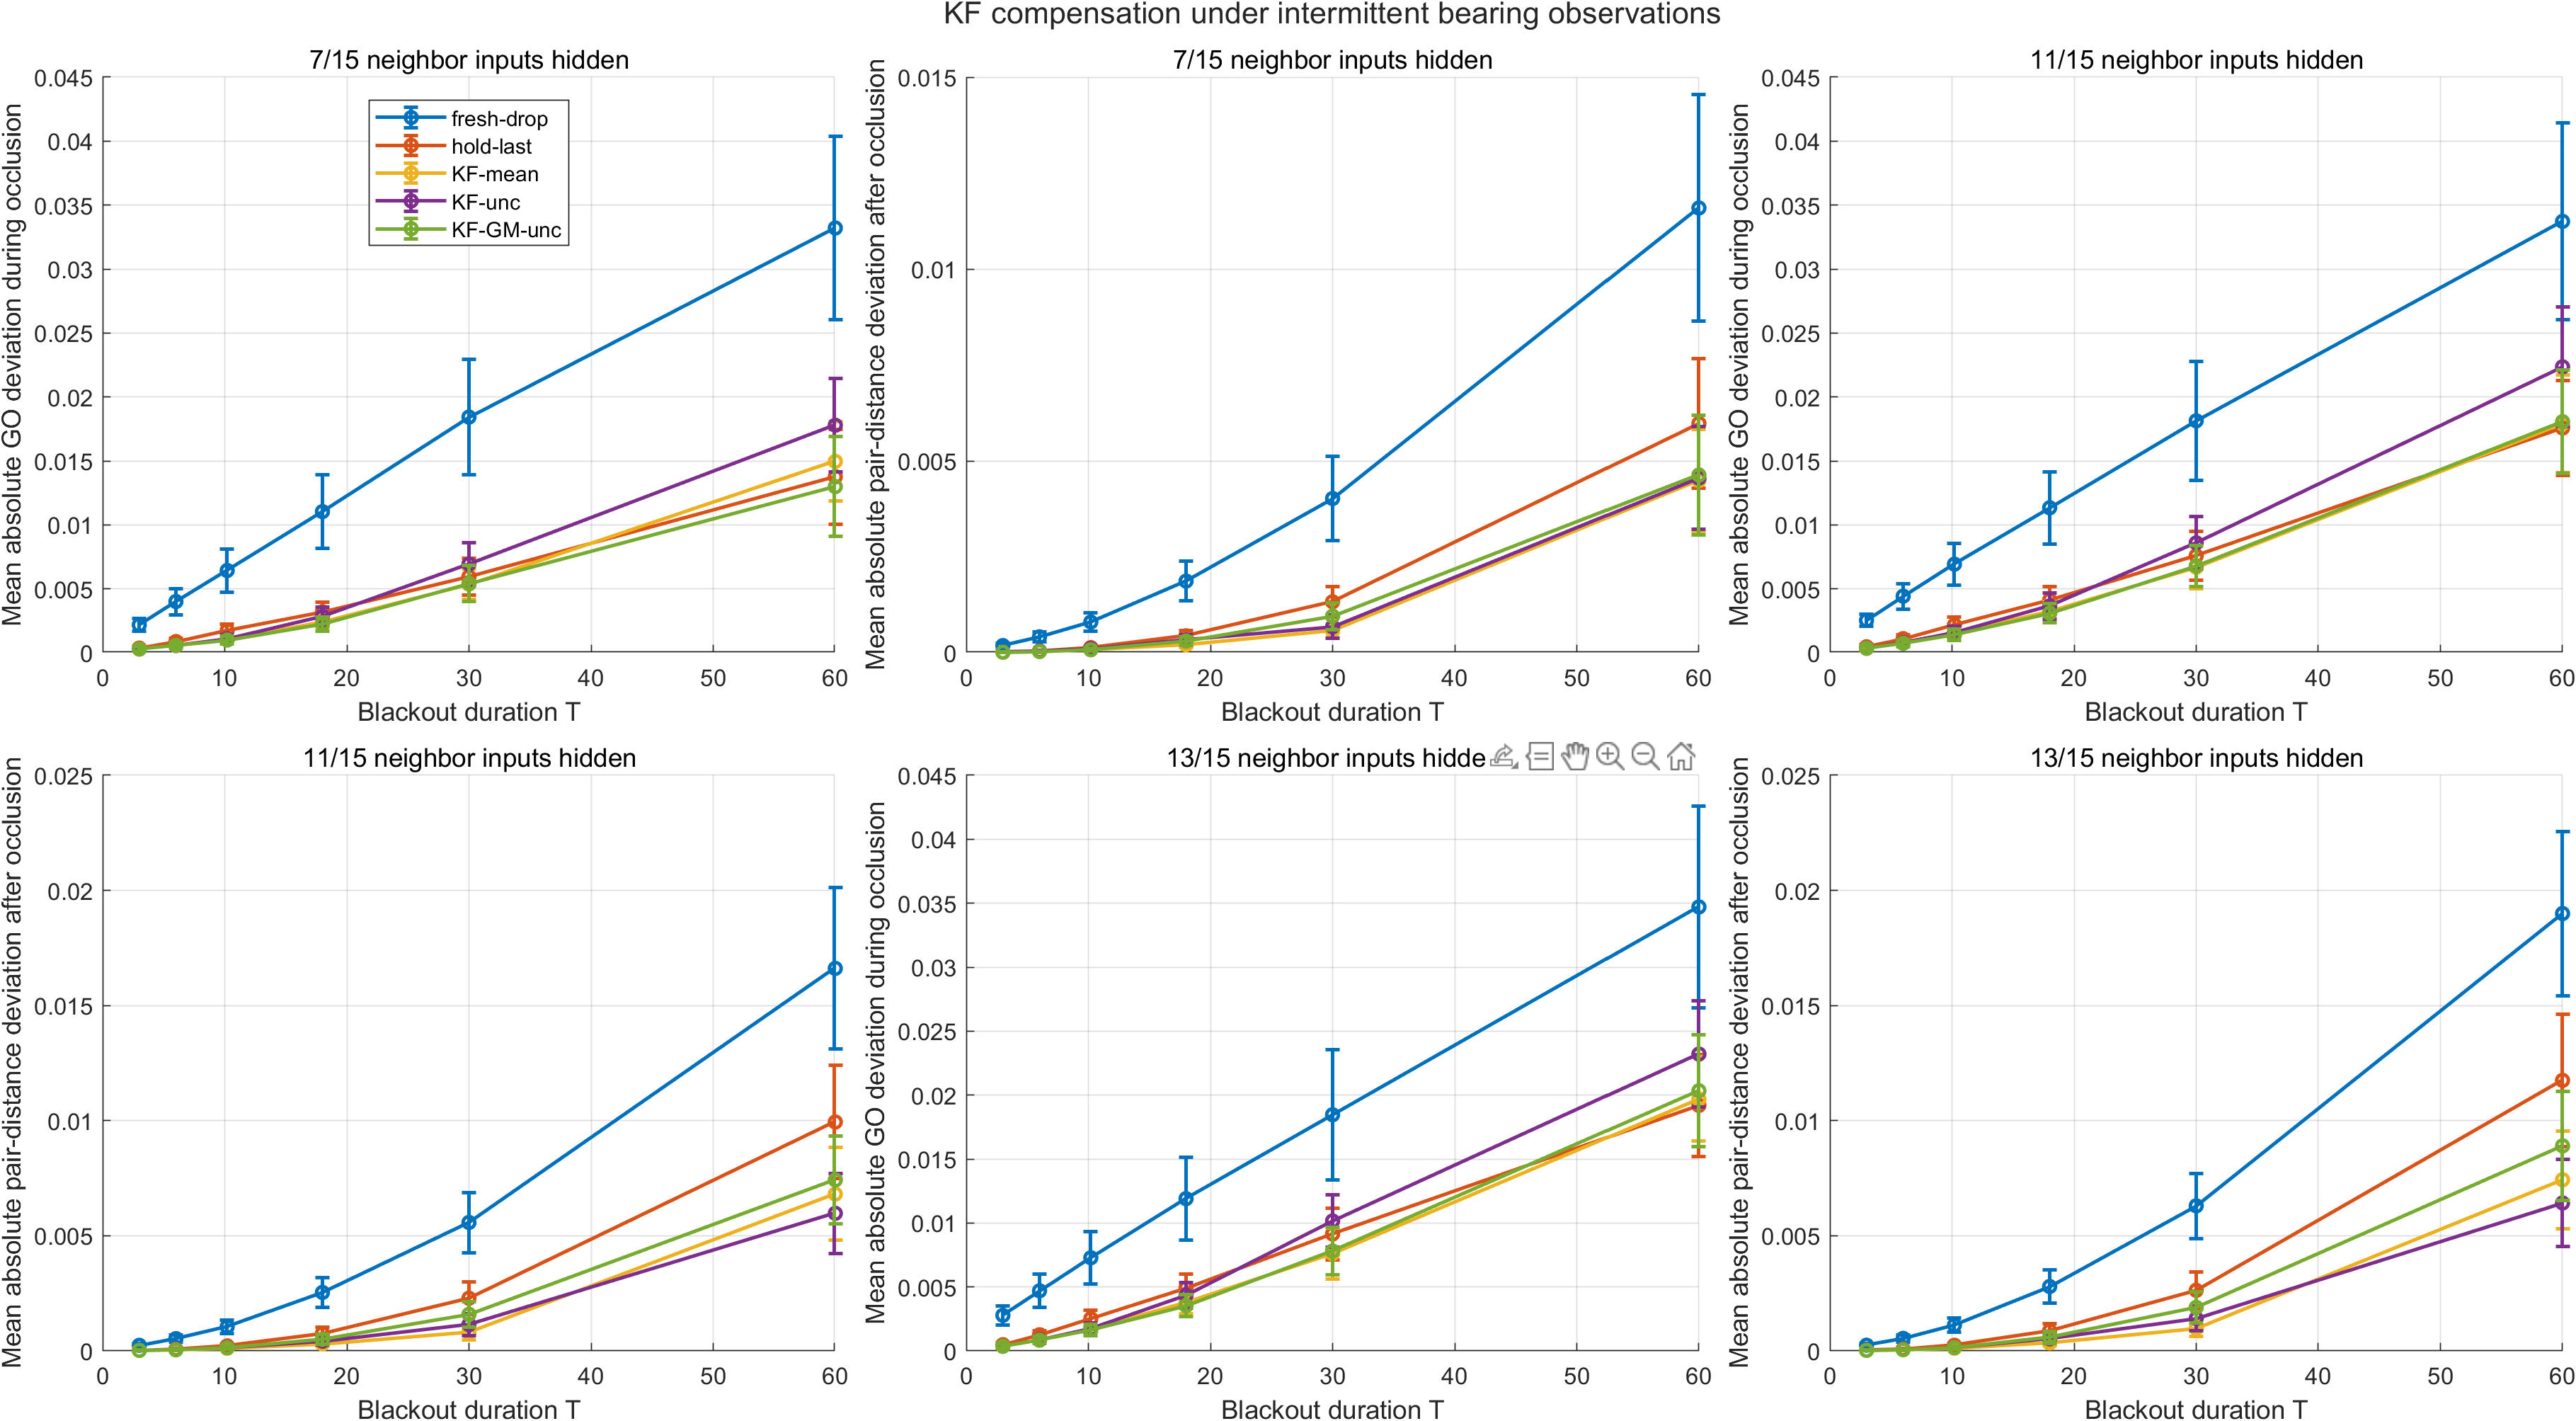
\includegraphics[width=0.98\linewidth]{kf-performance-summary.png}
 \caption{不同遮挡强度和时长下的绝对 GO 偏差与遮挡后距离偏差。误差线为种子均值的近似 $95\%$ 区间；表~\ref{tab:kf_go} 和表~\ref{tab:kf_pair} 给出逐条件配对 bootstrap 区间。}
 \label{fig:kf_performance}
\end{figure}

图~\ref{fig:kf_vs_hold} 直接给出各 Kalman 方法相对 hold-last 的配对差值。负值表示相对 hold-last 降低偏差。该图用于区分“保留旧方位已带来的收益”和“Kalman 外推或协方差卷积额外带来的收益”：短时遮挡中多数 Kalman 增量很小，中时遮挡中 KF-mean 和 KF-GM 对 GO 有可见增益，而 KF-uncertainty 的优势主要体现在长时间遮挡后的凝聚结构。

\begin{figure}[!tbp]
 \centering
 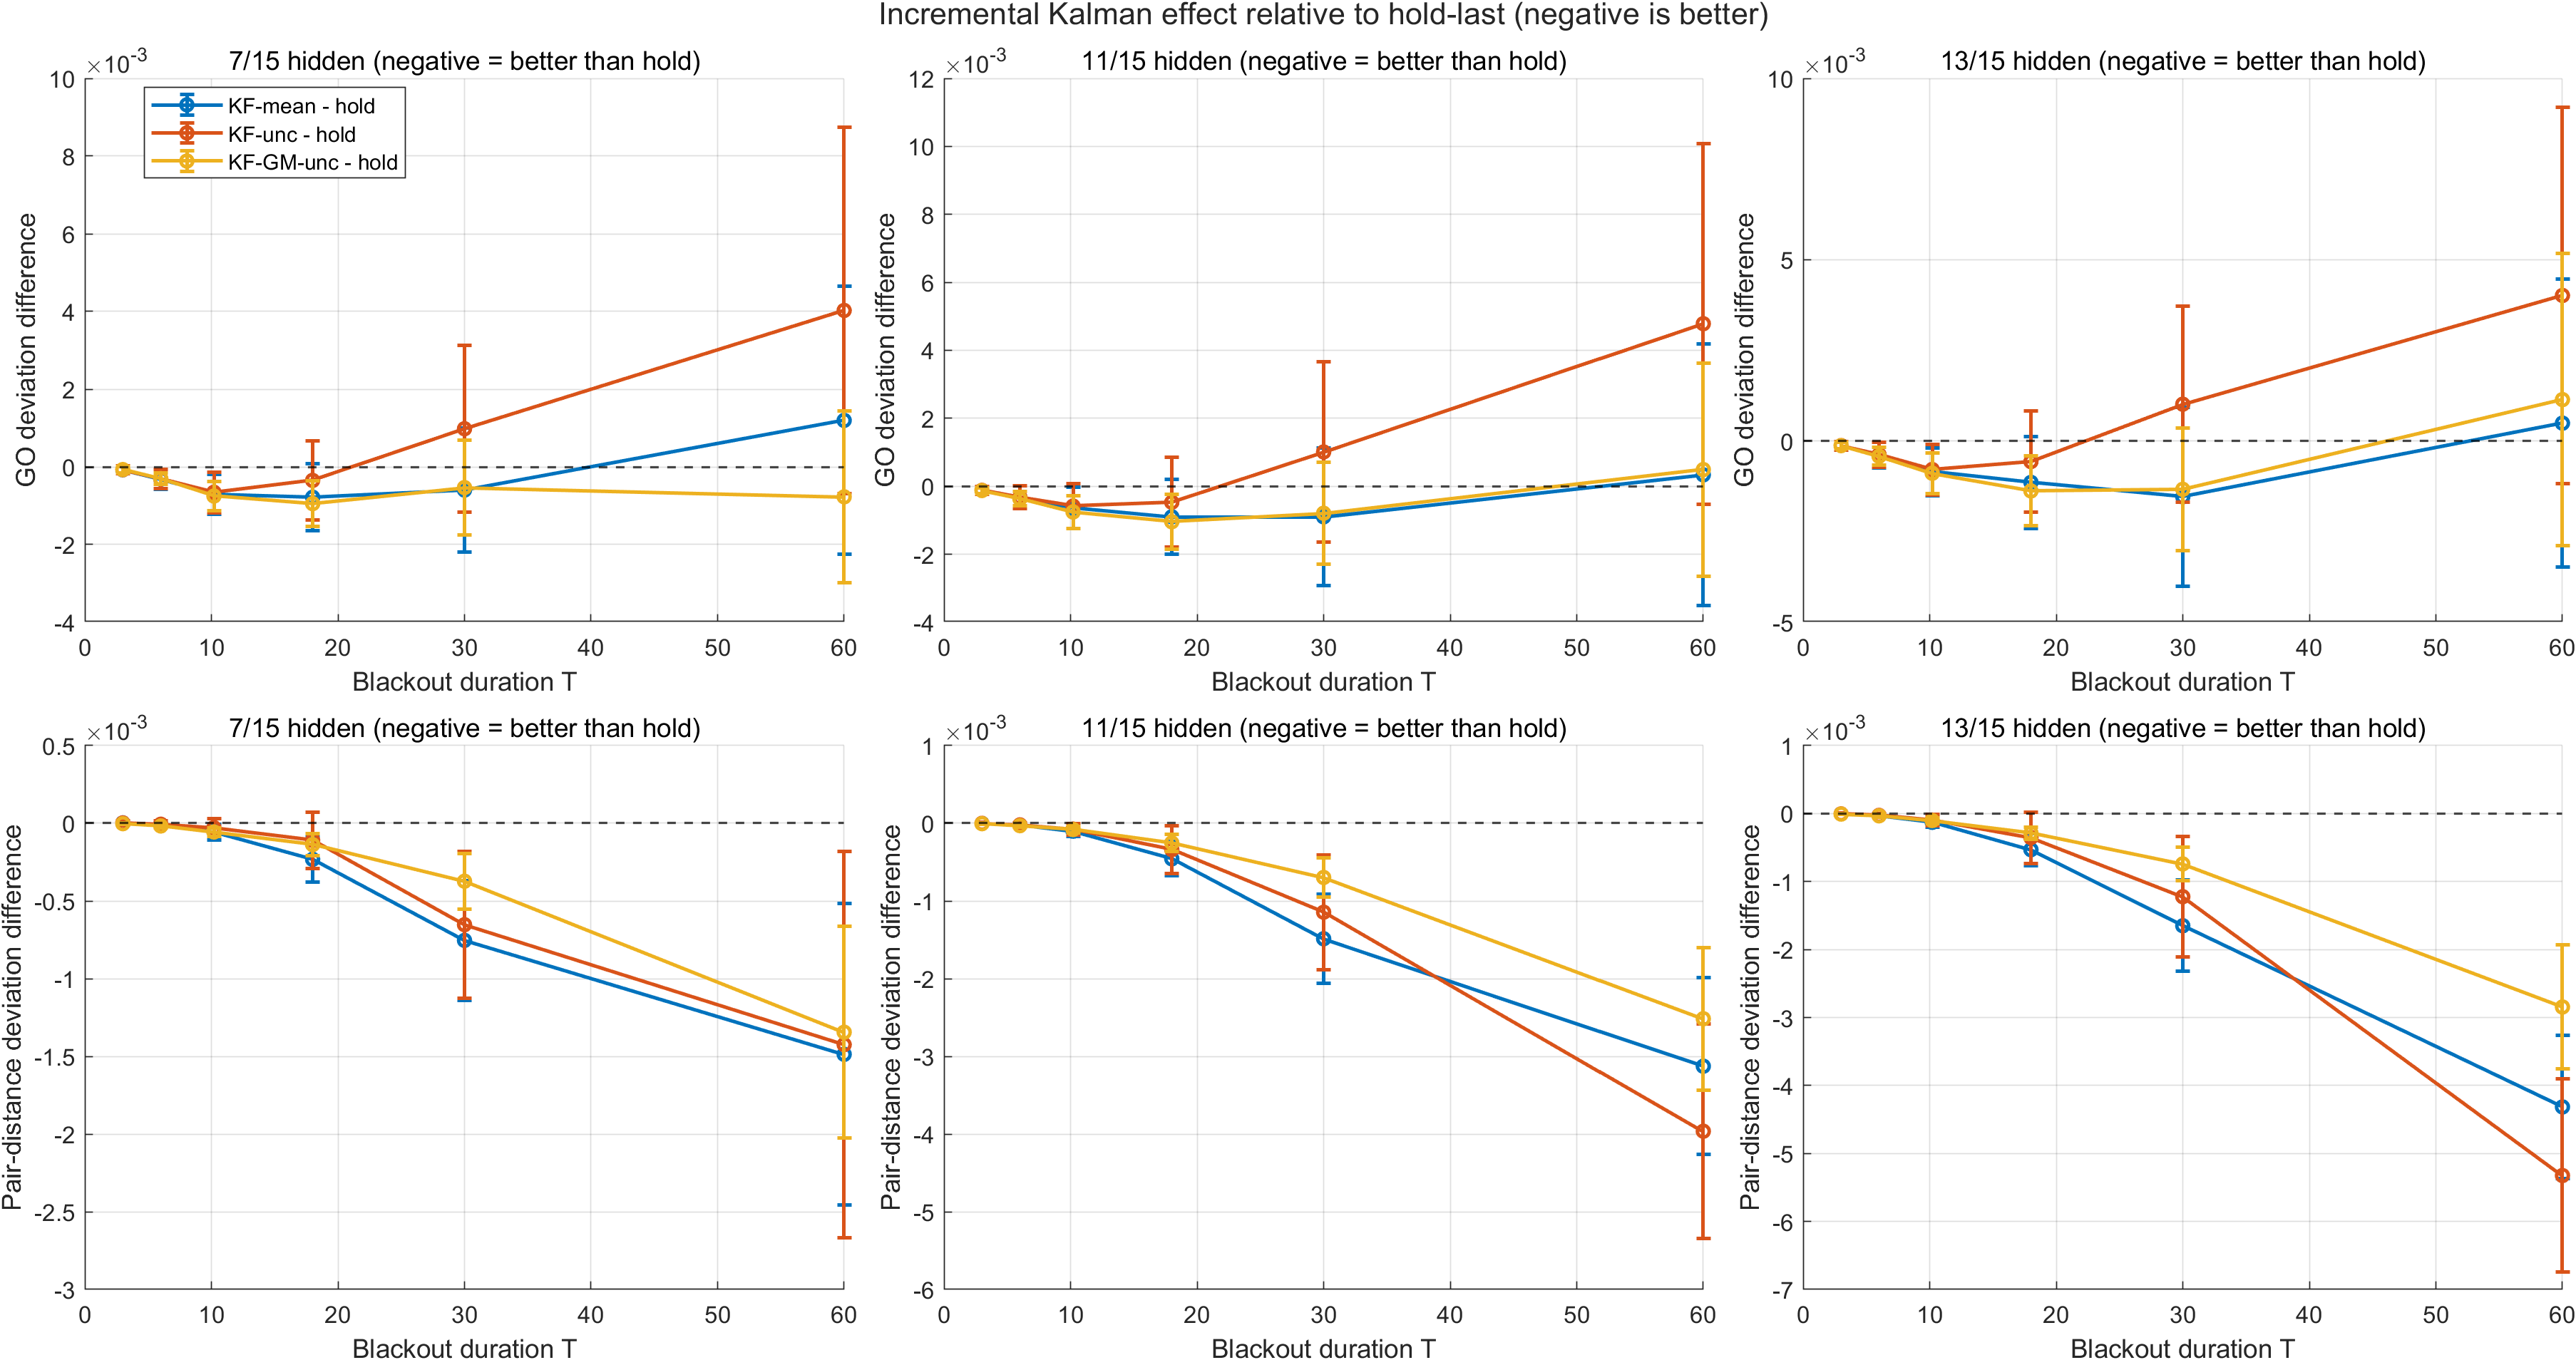
\includegraphics[width=0.98\linewidth]{kf-versus-hold.png}
 \caption{Kalman 方法相对 hold-last 的配对差值。横轴为遮挡时长，负值表示偏差低于 hold-last。}
 \label{fig:kf_vs_hold}
\end{figure}

\subsubsection{已有结果：受控转向下的配对群体响应}

为检验动态方向变化中的预测补偿，本文设置受控转向干预。首先从同一无遮挡检查点分叉；在遮挡开始前 $20$ 步（$6$ 个模型时间单位），对编号为 $1$--$3$ 的领航个体施加幅值 $0.08$ 的异中心旋转方向输入，领航方向以 $0.025$ rad/模型时间的角速度缓慢变化。遮挡在第 $201$ 步开始，期间领航个体继续转向；其余个体通过邻居方位输入跟随。Kalman 轨迹在遮挡前接收连续变化的方位观测并估计方位角速度，遮挡开始时跟随者仍处于向新共同方向调整的过程中。

受控转向实验仍比较 fresh-drop、hold-last、KF-mean、KF-uncertainty 和 KF-GM-uncertainty。每个方法与同一转向任务下的无遮挡控制轨迹配对。除绝对 GO、LO 和凝聚距离外，定义相对退化指标
\begin{equation}
 D_{\mathrm{GO}}^{\mathrm{rel}}=
 \frac{\operatorname{mean}_{k\in\mathcal K_o}
 |GO_{\mathrm{method}}(k)-GO_{\mathrm{control}}(k)|}
 {\operatorname{mean}_{k\in\mathcal K_o}|GO_{\mathrm{control}}(k)|},
\end{equation}
并以相同方式定义 $D_{\mathrm{LO}}^{\mathrm{rel}}$ 和遮挡后凝聚距离相对偏差 $D_{\mathrm{pair}}^{\mathrm{rel}}$，分别描述局部有序度和凝聚结构相对同任务无遮挡参考的变化。

图~\ref{fig:turn_timeline} 给出干预时序，图~\ref{fig:turn_relative} 给出 $30$ 个种子在隐藏 $11/15$ 条边条件下的响应。$T=3$ 和 $T=10.2$ 时，fresh-drop 的相对 GO 偏差分别为 $0.99\%$ 和 $2.82\%$，KF-GM-uncertainty 为 $0.13\%$ 和 $0.45\%$；遮挡后相对凝聚距离偏差由 $0.127\%$ 和 $0.605\%$ 降至 $0.0085\%$ 和 $0.090\%$。在持续方向变化条件下，KF-GM 补偿使群体有序度和距离结构更接近无遮挡参考。图中区间为 $30$ 个种子均值的逐条件近似 $95\%$ 区间。

\begin{figure}[!tbp]
 \centering
 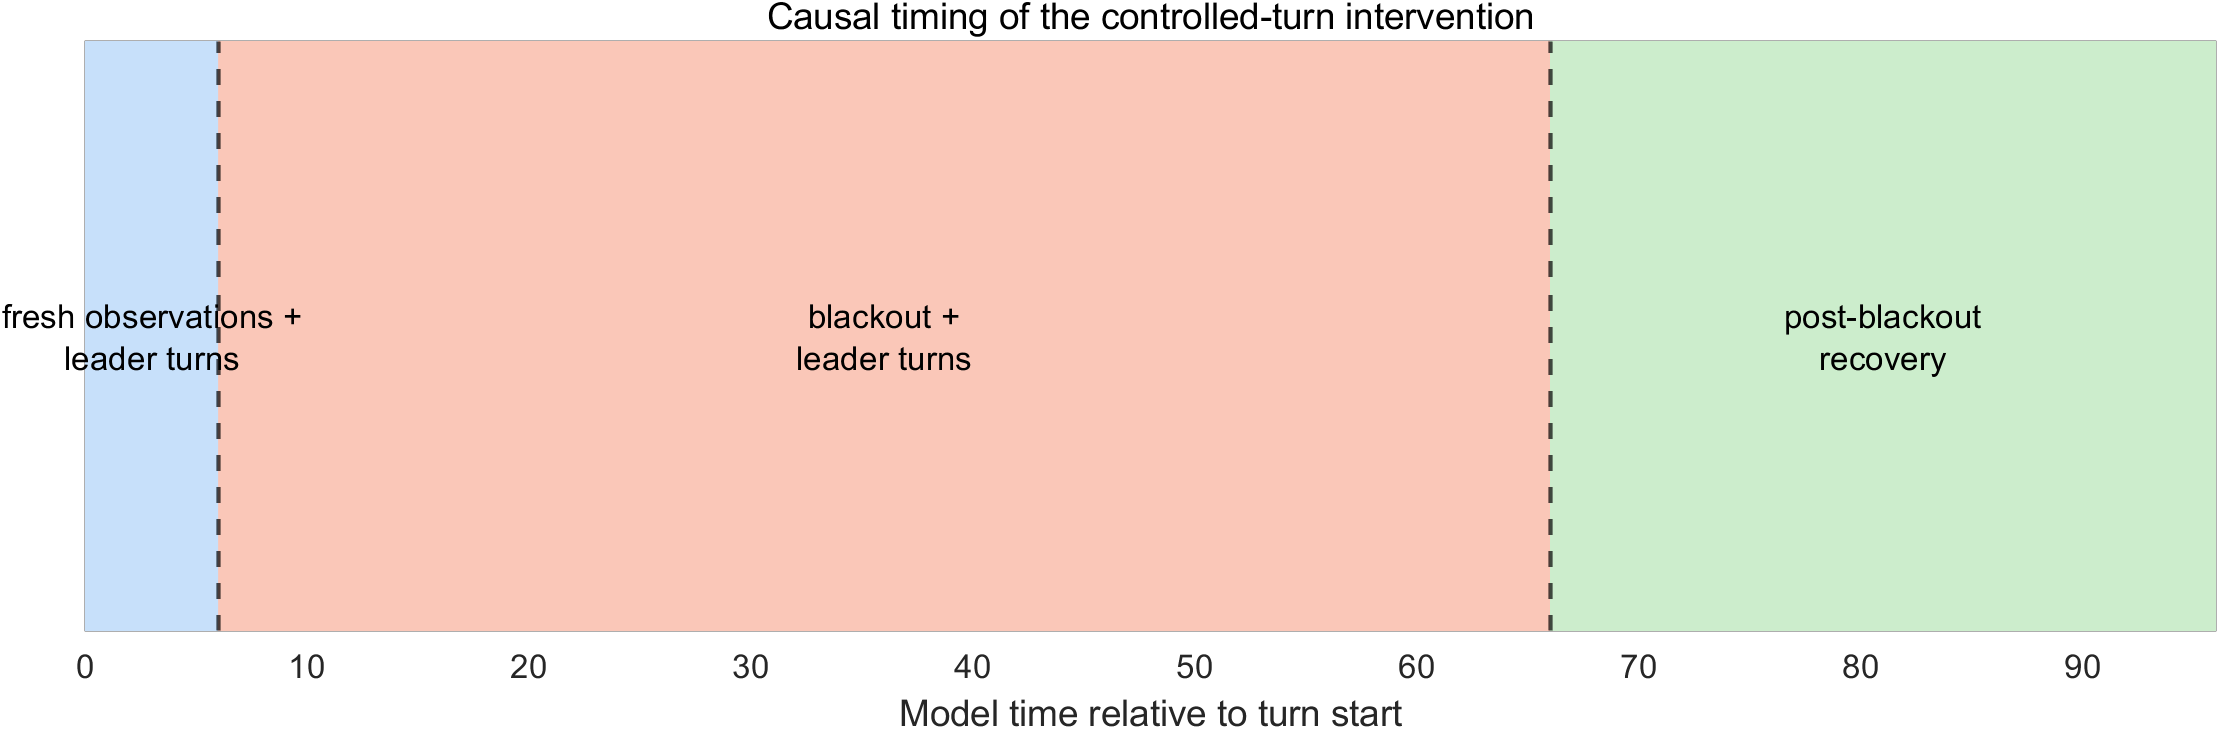
\includegraphics[width=0.82\linewidth]{intervention-timeline.png}
 \caption{受控转向实验时序：遮挡前先开始领航转向，随后进入连续遮挡和恢复窗口。}
 \label{fig:turn_timeline}
\end{figure}

\begin{figure}[!tbp]
 \centering
 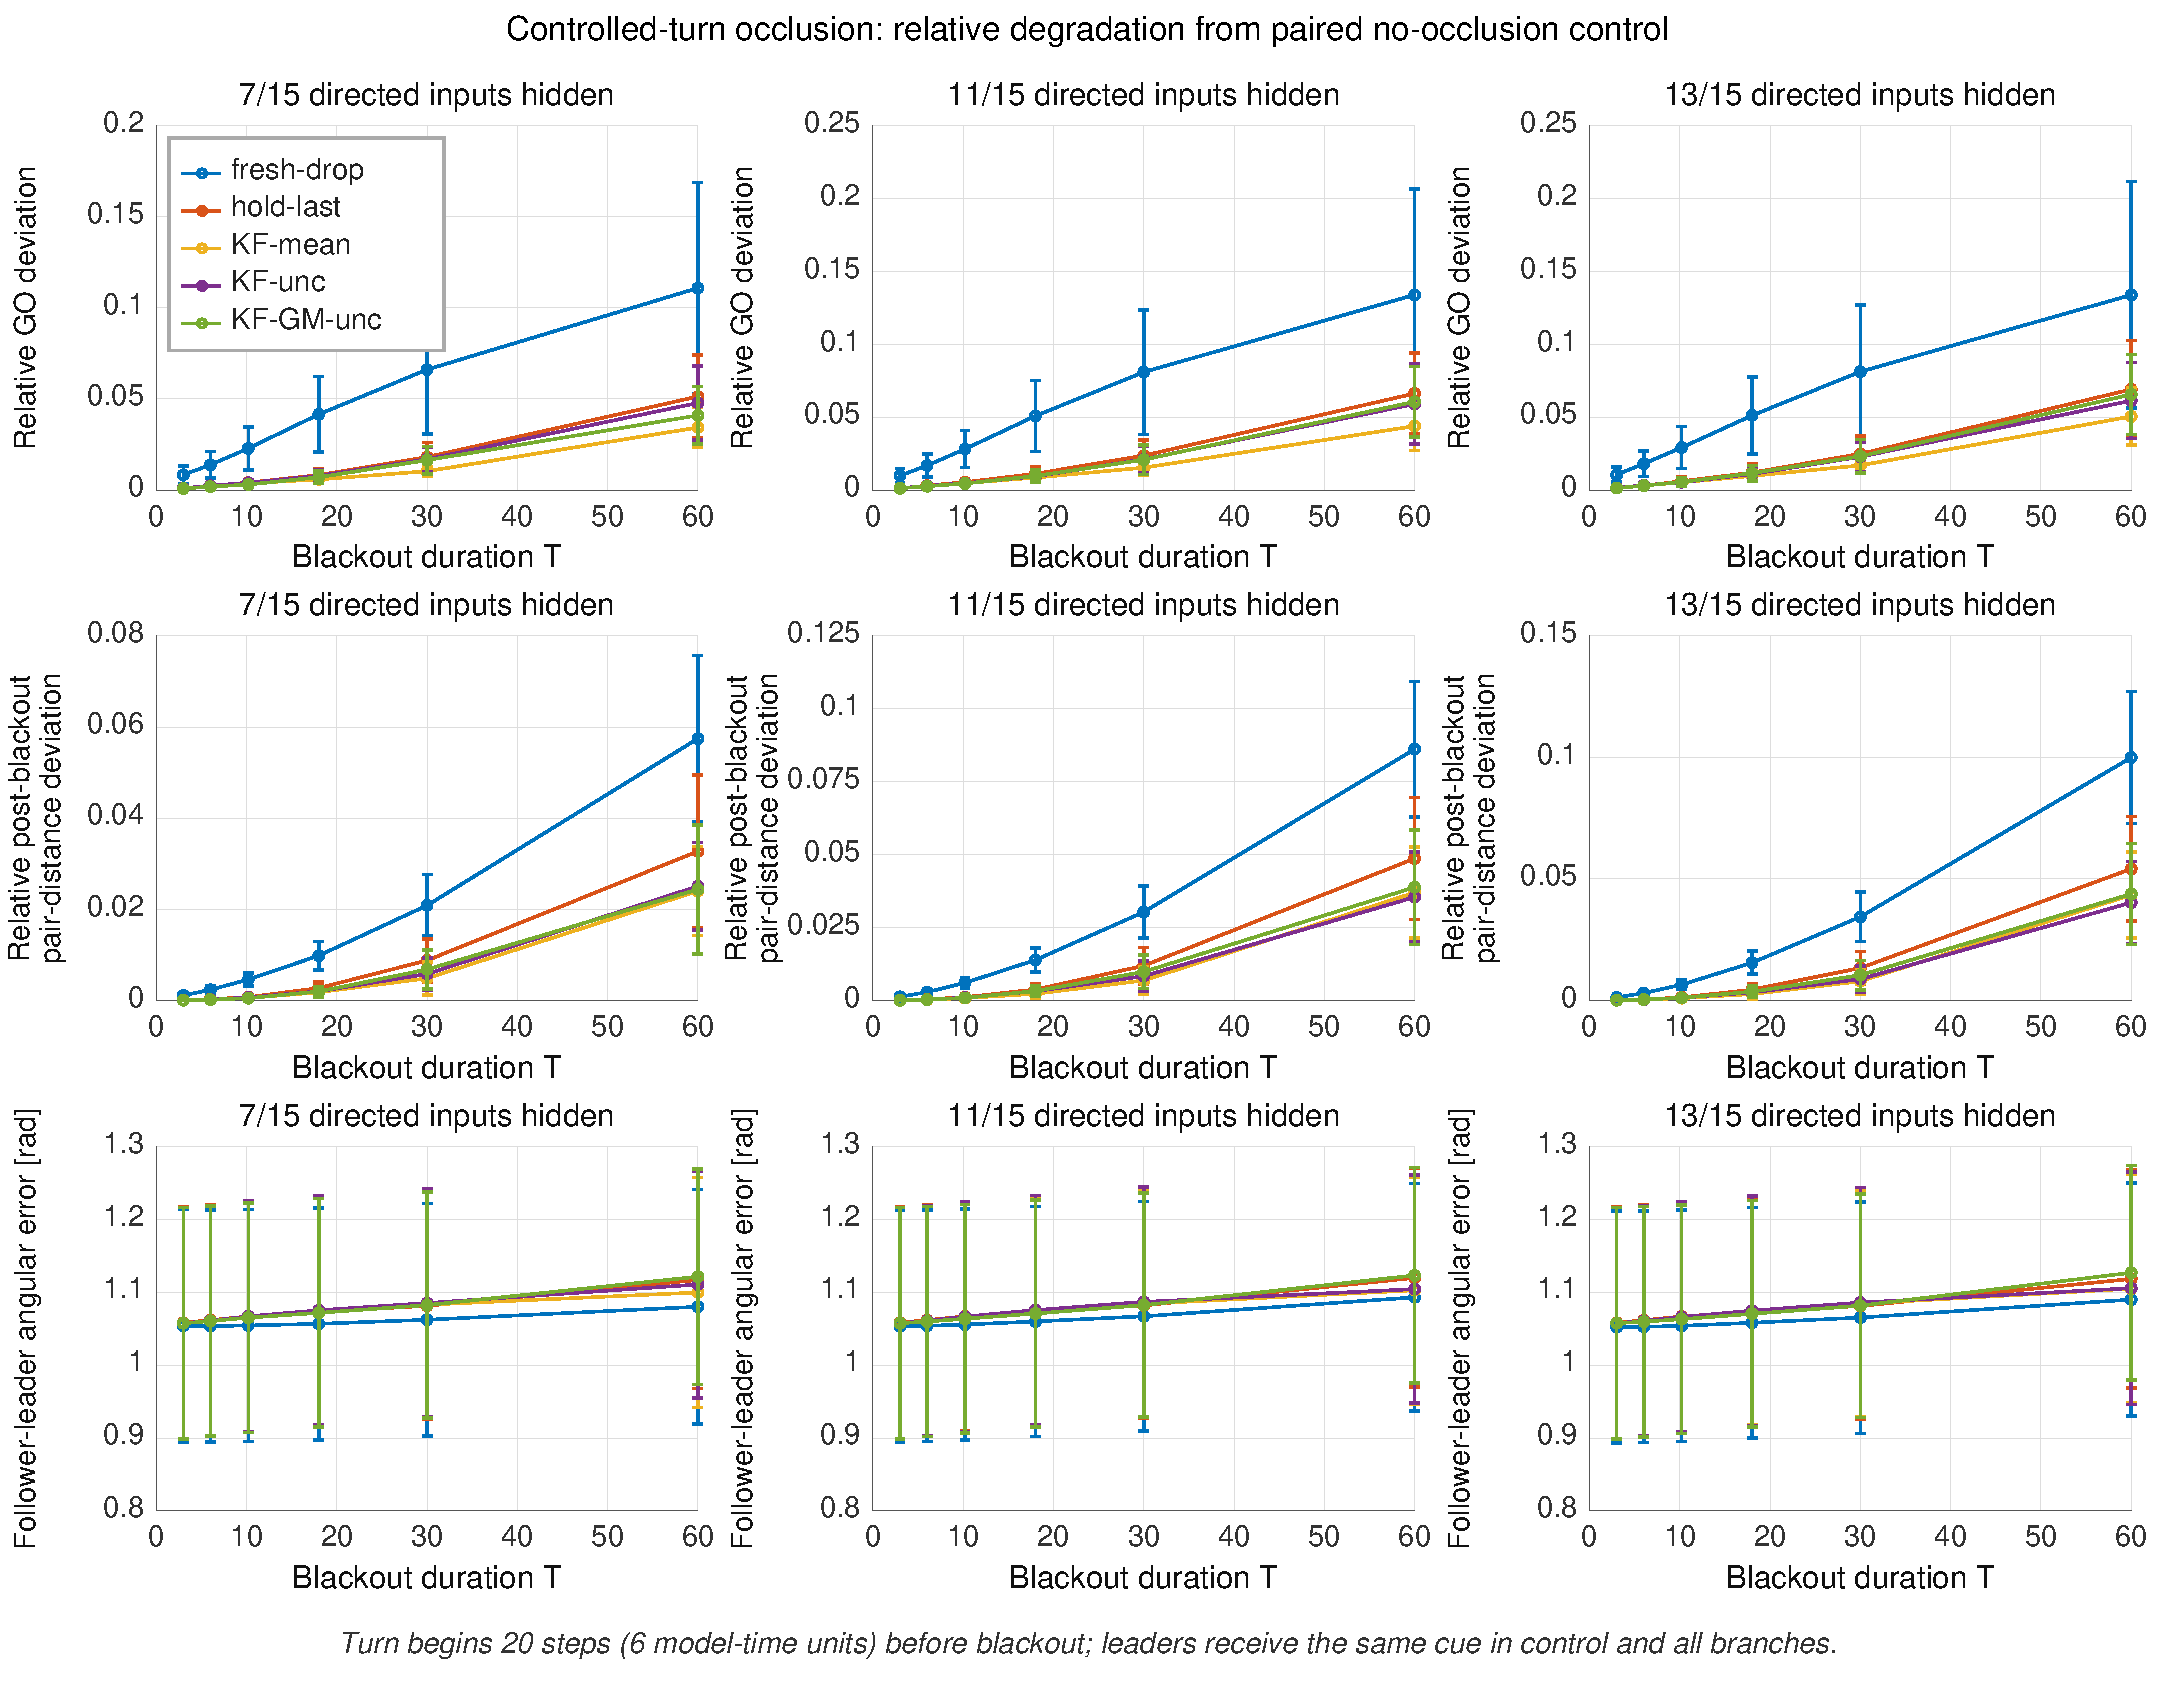
\includegraphics[width=0.98\linewidth]{relative-degradation-layout.pdf}
 \caption{受控转向下相对无遮挡控制的退化（完整 $30$ 个种子）。误差线为种子间近似 $95\%$ 置信区间。}
 \label{fig:turn_relative}
\end{figure}


\subsubsection{不同感知模型的群体响应参考}

Vicsek、Boids 和 Olfati--Saber 型规则分别使用邻居航向或相对位置等信息\upcite{Vicsek1995,Reynolds1987,OlfatiSaber2006}。表~\ref{tab:mainstream} 在各种模型的给定参数与感知配置下，报告种子 $101$--$105$、$T=30$、隐藏 $7/15$ 条输入时的平均有序度与最小距离，作为不同交互机制的描述性参考。

\begin{table}[!tbp]
\centering\small
\caption{不同感知配置下的群体响应均值，$n=5$。GO 损失为配对无遮挡值减遮挡值，最小距离按全仿真记录统计。}
\label{tab:mainstream}
\begin{tabular}{lrrr}
\toprule 模型 & 遮挡期 GO & GO 损失 & 最小距离$/L$\\\midrule
本文 KF-unc & 0.729 & $-0.0014$ & 0.00056\\
Vicsek（航向） & 1.000 & 0 & 0.00760\\
Boids（位置与航向） & 0.975 & 0.0038 & 0.00773\\
Olfati--Saber 型（位置与航向） & 0.911 & 0.0368 & 0.00764\\\bottomrule
\end{tabular}
\end{table}

相对位置输入为排斥与势函数作用提供几何信息，方位神经场则通过方向核组织社会输入。表中的 GO 与最小距离分别描述方向一致性和空间接近程度，反映了不同感知与交互机制下的群体响应。





\subsubsection{后续实验：重建配置冻结后的条件边界}\label{sec:challenge3_plan}
边界实验将按“冻结重建配置--分因素扫描--独立边界评价”的顺序开展。挑战2的分层结果确定运动模型、过程噪声、周期输入形式与门控后，首先在共同群体参数下扫描 $k_{\rm fresh}$，再交叉考察均匀、集中和多峰方位结构，最后增加连续缺失时长 $T$。每组条件均配对设置无遮挡参考、删除输入、方位保持和预测补偿，并记录实际激活边数、输入强度、完整场误差与群体指标。

评价将同时给出 $D_{GO}$、$D_{LO}$ 和 $D_{d/L}$ 的响应曲面，以及式\eqref{eq:v7_boundary_event}的联合事件比例与区间。预先固定容许偏差、概率目标和统计窗口后，采用独立种子估计各方位结构及缺失时长下的新鲜输入边界，进一步比较预测相对方位保持所减少的新鲜输入需求。方向变化和恢复过程沿用相同配对组织，补充逐时刻联合达标比例、首次越界时间和恢复时间的专门统计。



\begin{table}[!htbp]
\centering\small
\caption{挑战3后续条件边界实验的递进安排}
\label{tab:boundary_experiment_plan}
\begin{tabular}{>{\raggedright\arraybackslash}p{0.16\linewidth}
                >{\raggedright\arraybackslash}p{0.40\linewidth}
                >{\raggedright\arraybackslash}p{0.34\linewidth}}
\toprule
阶段 & 条件组织 & 拟形成的结果\\
\midrule
分因素定位 & 固定重建配置，分别改变新鲜数量、方位结构和缺失时长 & 各单项响应、输入强度和激活边记录\\[3pt]
联合扫描 & 在共同条件下交叉数量、方位与时长，保留无遮挡和记忆对照 & 群体响应曲面及联合事件比例\\[3pt]
独立评价 & 冻结容许量、窗口和概率目标，在独立种子上评价 & 条件边界、区间及预测相对方位保持的边界差\\
\bottomrule
\end{tabular}
\end{table}
边界扫描将同时包含方向稳定、方向变化和自主相互转向场景，按场景等权或预先确定的权重汇总，并同时展示分层结果。由此在多种运动与方位条件下评价群体响应，形成与挑战1综合选型、挑战2分层验证相衔接的整体评价。


\section{讨论}

\subsection{挑战1：经验量化中的强度与方向信息}
总强度 $A=n\bar w$ 描述数量和单边强度的合成作用，二维合方向补充输入的方向信息。所选 $q=1$ 保留各方位的强度，通过方向通道区分侧向作用。速度--活动评分下的选择与宽高斯在速度、场误差上的表现，共同表明经验公式的形式应与目标响应对应。附录的多阶结构分析进一步解释了多峰输入对低维描述的要求。

\subsection{挑战2：从方位预测到周期输入重建}
方位后验经过周期核叠加后形成神经场输入，重建效果由误差方向、预测方差、核宽度及邻居方位分布共同决定。五种子中心条件中，输入误差降低与方位 RMSE 的种子异质性同时出现，覆盖率和 NIS 又提供了模型与方差校准的诊断。共同边、共同窗口和组件对照的分层设计，将进一步建立预测精度、方差校准和输入响应之间的定量关系，并为群体实验提供统一的重建配置。

\subsection{挑战3：从闭环响应到条件边界}
共同检查点分叉将群体响应与同一历史状态联系起来，GO、LO 和凝聚距离描述方向协调与空间结构的不同侧面。现有遮挡和转向条件中的配对响应，为数量--方位--时长坐标下的边界实验提供起点。边界评价将沿挑战2冻结后的配置展开，以独立种子、明确容许量和联合事件刻画条件范围；总强度与方位覆盖的分层记录使各输入因素的作用保持可解释。

\section{结论}

本文围绕社会输入量化、缺失方位预测与输入重建、群体闭环响应三条主线，建立从邻居信息到群体运动的研究框架。

在社会输入量化方面，比较六类正值经验公式，统一考虑数量、单边强度和相对方位。速度--活动评分选出 $q=1$，其描述量简化为总强度和二维合方向；在 $400$ 组独立几何中，两项末段响应预测 RMSE 较固定指数分别降低 $2.36\%$ 和 $4.17\%$，宽高斯在速度和场重建目标上具有更低误差。

在预测与输入重建方面，方位--角速度状态、协方差传播和周期核卷积共同延续缺失期间的方向输入。理论给出指定后验下的条件均方重建性质、方向谐波衰减和有限时间扰动界。五种子中心条件中，KF-mean 相对方位保持的同状态输入误差降低 $61.8\%$；分层验证设计进一步围绕共同样本评价方位精度、协方差校准及输入重建，形成群体实验所需的配置依据。

在群体响应方面，共同检查点与三十种子配对实验量化了遮挡及受控转向中的有序度和凝聚偏差，预测相对方位保持的增量随缺失时长和指标变化。围绕新鲜输入数量、方位结构和缺失时长建立条件边界定义，并给出在挑战2配置冻结后递进开展的边界实验方案，将重建输入的局部作用连接到群体运动的条件范围。

\section*{数据与代码可用性}
本文分析使用的结果批次及对应数据目录如下：
\begin{itemize}[nosep,leftmargin=2em]
\item 挑战1经验公式选型：\texttt{social-input-positive-v2-20261014}；
\item 方向结构补充回放：\texttt{challenge1-final-v1-20261015}；
\item 五种子机制实验：\texttt{pilot\_seed1to5\_v1}；
\item 扩展缺失时长：\texttt{paper-kf-extended-v3/full}；
\item 受控转向：\texttt{turn-occlusion-pilot-v1/full}。
\end{itemize}
论文源码及配套图见仓库 \url{https://github.com/PatrickStar-cmd/Flocking_Study} 的 \texttt{paper/} 目录。经验公式目录包含冻结方案、数据分区、候选参数搜索、读出系数和独立测试预测。复核目录为：
\begin{itemize}[nosep,leftmargin=2em]
\item 公式图表与数值：\path{reviews/challenge1-formula-selection-20261018/}；
\item V6文字与实现：\path{reviews/challenge1-prose-20261018/}；
\item V7结构重排与编译复核：\path{reviews/paper-v7-structure-20261020/}；
\item 结构回放：\path{reviews/challenge1-final-20261015/}。
\end{itemize}
其他批次按其汇总 CSV 分析。复核记录包含输入 SHA256、代码版本及编译记录。

\appendix
\section{经验公式的实现与补充分析}
\subsection{拟合与统计细节}\label{app:empirical_details}
四个描述量展开为 $14$ 个一次和二次项。各形式采用同一展开规则；由于代数依赖，选定的无衰减、余弦和 Cauchy 表示有效秩为 $9$，指数、高斯和 Laplace 为 $14$。正则化网格为 $\{10^{-4},10^{-3},10^{-2},10^{-1},1\}$，各选定形式均取 $10^{-4}$。速度预测向量的模限制为 $1$，速率与活动限制在 $[0,1]$，零输入对应零响应。输入由 PCG64 生成并序列化，完整种子、随机输入与模型参数随代码保存。

以七类等权的训练期望 $\mathbb E_{\rm tr}$ 定义式\eqref{eq:empirical_selection_score}的尺度：
\begin{equation}
 s_v^2=\mathbb E_{\rm tr}\|\boldsymbol y_v-\mathbb E_{\rm tr}\boldsymbol y_v\|_2^2,\qquad
 s_a^2=\mathbb E_{\rm tr}(y_a-\mathbb E_{\rm tr}y_a)^2.
\end{equation}
测试误差按几何和条件汇总。设第 $f$ 类有 $G_f$ 组几何，则
\begin{equation}
 \operatorname{RMSE}_{v}(q)=\left[\frac17\sum_{f=1}^{7}\frac1{G_f}\sum_{g=1}^{G_f}
 \frac1{24}\sum_{c=1}^{24}\|\widehat{\boldsymbol y}^{(q)}_{fgc,v}-\boldsymbol y_{fgc,v}\|_2^2\right]^{1/2}.
 \label{eq:challenge1_vector_error}
\end{equation}
活动误差采用标量平方差。输入场解码器以相同描述量另行拟合，输出经非负截断后乘总强度，得到重建场。

\subsection{方向结构与缺失输入的补充推导}\label{app:direction_structure}
定义圆周矩及归一化矩
\begin{equation}
 Z_{i,\ell}=\sum_jw_{ij}e^{\mathrm i\ell\delta^\theta_{ij}},\quad
 Z_{i,0}=A_i=n_i\bar w_i,\qquad\varrho_{i,\ell}=Z_{i,\ell}/A_i,
 \label{eq:strength_circular_moments}
\end{equation}
无输入时令 $\bar w_i=Z_{i,\ell}=\varrho_{i,\ell}=0$。$q=1$ 时 $\boldsymbol V_i=[\Re Z_{i,1},\Im Z_{i,1}]^\top$，因而保持全部方位的强度并用一阶矩描述合方向。等强度前后双峰与左右双峰的一阶矩均为零，二阶矩分别为 $A_i$ 与 $-A_i$；这说明同一低维经验量仍可对应不同输入结构。

用原周期高斯核 $g_{\sigma_s}$ 表示参考轴坐标下的完整输入及其 Fourier 系数：
\begin{equation}
 I_i^{\rm ref}(\xi)=\sum_jw_{ij}g_{\sigma_s}(\xi-\delta^\theta_{ij}),\qquad
 c_\ell=\frac1{2\pi}\int_{-\pi}^{\pi}g_{\sigma_s}(\xi)e^{-\mathrm i\ell\xi}\,\mathrm d\xi.
 \label{eq:social_field_fourier_coefficients}
\end{equation}
\begin{equation}
 I_i^{\rm ref}(\xi)=c_0A_i+2\sum_{\ell\ge1}c_\ell
 [\Re Z_{i,\ell}\cos(\ell\xi)+\Im Z_{i,\ell}\sin(\ell\xi)].
 \label{eq:social_field_moment_expansion}
\end{equation}
在归一化 $L^2$ 范数 $\|f\|_{L^2_*}^2=(2\pi)^{-1}\int_{-\pi}^{\pi}|f|^2\,\mathrm d\xi$ 下，原始 $p$ 阶谱截断满足
\begin{equation}
 \|I_i^{\rm ref}-I_i^{[p]}\|_{L^2_*}^2
 =2\sum_{\ell>p}|c_\ell|^2|Z_{i,\ell}|^2
 \le2A_i^2\sum_{\ell>p}|c_\ell|^2.
 \label{eq:social_field_parseval_tail}
\end{equation}
同一参考轴下，两组完整输入的差满足
\begin{equation}
 \|I_i^{\rm ref}-\widehat I_i^{\rm ref}\|_{L^2_*}^2
 =c_0^2|A_i-\widehat A_i|^2+2\sum_{\ell\ge1}|c_\ell|^2|Z_{i,\ell}-\widehat Z_{i,\ell}|^2.
 \label{eq:social_field_error_decomposition}
\end{equation}
上述关系由 Fourier 正交性和 $|Z_{i,\ell}|\le A_i$ 得到，说明不同方向结构如何影响完整输入场。


\paragraph{缺失信息的量化分解}
在同一参考轴下，以 $(A_i,Z_{i,\ell})$ 和 $(\widehat A_i,\widehat Z_{i,\ell})$ 分别表示完整与可用输入。式\eqref{eq:social_field_error_decomposition}将场误差分为零阶幅值差和各阶方向矩差，其中
\begin{equation}
 \Delta Z_{i,\ell}=(A_i-\widehat A_i)\varrho_{i,\ell}
 +\widehat A_i(\varrho_{i,\ell}-\widehat\varrho_{i,\ell}).
 \label{eq:missing_input_decomposition}
\end{equation}
删除集合 $\mathcal H_i$ 时，幅值损失为 $\Delta A_i=\sum_{j\in\mathcal H_i}w_{ij}$，方向矩损失为 $\Delta Z_{i,\ell}=\sum_{j\in\mathcal H_i}w_{ij}e^{\mathrm i\ell\delta^\theta_{ij}}$。保持旧方位维持总幅值，其误差来自方向矩的变化。若方位后验为包裹正态分布，则
\begin{equation}
 \mathbb E[Z_{i,\ell}\mid\mathcal Z_i]
 =\sum_jw_{ij}\exp\!\left[\mathrm i\ell(\mu_{ij}-\phi_i^{\rm ref})-\frac{\ell^2V_{ij}}2\right].
\end{equation}
该关系把预测均值与方差分别映射为方向相位与各阶幅值衰减，与第~\ref{sec:prediction_method} 节的周期核卷积相联系。

\subsection{方向表示与时变输入的补充检验}\label{app:structure_experiment}
在相同末段响应预测任务中，仅用 $[A,S_{\exp}]$ 的速度 RMSE 为 $0.236318$，高于保留方向通道的固定指数 $0.125627$；二阶结构对照为 $0.114335$，采用五个原始通道和 $20$ 个二次展开特征。它们分别说明方向信息与多峰结构的作用。去掉 $q=1$ 的重复 $S=A$ 列后，一阶矩对照的速度 RMSE 为 $0.12266127$，与主实现仅相差 $2.3\times10^{-7}$，重复列对本次比较的影响很小。

另一个预先冻结的结构回放批次使用 $420$ 组新几何，将描述量解码为输入场后再运行原神经动力学，评价完整 $120$ 步速度轨迹。其中 M1 表示一阶矩，M2 表示一阶加二阶矩，M13 表示一阶加三阶矩。零初态静态条件下，M2 相对 M1 与同维数 M13 的轨迹 RMSE 分别低 $40.4\%$、$39.0\%$；预热后持续变形时则比 M13 高 $42.7\%$。该批次评价完整轨迹的输入重建效果，显示方向阶次的作用随输入结构和神经初态变化。


额外 $172$ 个预定诊断条件覆盖全角度、弱强度与对称性。弱强度位于训练范围之外；精确对称输入的方向响应对网格和极小初始扰动敏感，因而同时报告总体活动。相关结果随主实验数据保存。

\section{预测重建与有限时间响应的理论分析}\label{sec:theory}

间歇方位观测下的异中心神经场需要同时处理方向估计、预测不确定性和社会输入缺失。为刻画这些因素之间的关系，本节以方位后验、周期社会输入和神经场状态为理论对象，组织以下两层误差分析：
\[
\begin{gathered}
\text{指定方位后验}\;\longrightarrow\;\text{同状态输入重建误差},\\
\text{闭环实际输入差}\;\longrightarrow\;\text{神经场状态差}\;\longrightarrow\;\text{速度与位置偏差}.
\end{gathered}
\]

理论分析包含四个相互衔接的层次：首先证明协方差感知输入在相同有效轨迹集合上的条件均方最优性，并量化均值输入的额外重建风险；其次分解有效集合内的方向预测误差与集合外的遗漏输入；随后建立方位方差与周期方向谐波衰减的解析关系；最后在神经场推进映射满足 Lipschitz 条件时，给出实际输入扰动向神经状态、速度及位置偏差传播的有限时间界。

\subsection{理论对象、符号与适用条件}

考虑智能体 $i$ 在时刻 $k$ 的观测历史 $\mathcal Z_i(0:k)$。记异中心神经场模型中的有向邻居集合为 $\mathcal B_i(k)$，由历史观测确定、已经初始化且当前满足输入有效性条件的集合为
\[
\mathcal S_i(k)\subseteq\mathcal B_i(k).
\]
前者表示参考社会输入包含的邻居，后者表示当前预测器维护的有效轨迹。协方差感知输入在 $\mathcal S_i(k)$ 上重建方向信息，集合差 $\mathcal B_i(k)\setminus\mathcal S_i(k)$ 对应遗漏输入。

对环形神经场的方向单元 $\alpha_m$，定义周期方位核
\begin{equation}
 g_\sigma(x)=\exp\!\left[-\frac{\operatorname{wrap}(x)^2}{2\sigma_s^2}\right],
 \qquad
 \operatorname{wrap}(x)=\operatorname{mod}(x+\pi,2\pi)-\pi .
 \label{eq:v2_kernel}
\end{equation}
其中 $0<\sigma_s\leq\pi$。圆周距离记为
\begin{equation}
 d_{\Sone}(a,b)=|\operatorname{wrap}(a-b)|.
 \label{eq:v2_circle_distance}
\end{equation}

对 $j\in\mathcal B_i(k)$，令 $\Theta_{ij}(k)\in\Sone$ 表示真实世界方位；对 $j\in\mathcal S_i(k)$，方位预测器给出预测均值 $\mu_{ij}(k)$ 和方位方差 $V_{ij}(k)$。在当前观测历史条件下，假定有效轨迹的方位边缘后验满足
\begin{equation}
 \Theta_{ij}\mid\mathcal Z_i\sim\operatorname{WN}(\mu_{ij},V_{ij}),
 \qquad j\in\mathcal S_i,
 \label{eq:v2_wn_assumption}
\end{equation}
其中 $\operatorname{WN}$ 表示包裹正态分布，以下简写 $\mathcal Z_i=\mathcal Z_i(0:k)$。$(\mu_{ij},V_{ij})$ 在本节中为该条件分布的参数。推导采用条件期望线性性与三角不等式，对邻居间的条件相关性保持一般性；局部展开分支、身份关联与输入有效性满足前述假设。

定义有效轨迹集合上的理想社会输入
\begin{equation}
 J_{im}^{(\mathcal S)}=h_0\sum_{j\in\mathcal S_i}g_\sigma(\alpha_m-\Theta_{ij}),
 \qquad
 J_i^{(\mathcal S)}=[J_{i0}^{(\mathcal S)},\ldots,J_{i,M-1}^{(\mathcal S)}]^{\top}.
 \label{eq:v2_tracked_ideal}
\end{equation}
完整邻居集合上的新鲜参考输入定义为
\begin{equation}
 J_{im}^{(\mathcal B)}=h_0\sum_{j\in\mathcal B_i}g_\sigma(\alpha_m-\Theta_{ij}),
 \qquad
 J_i^{(\mathcal B)}=[J_{i0}^{(\mathcal B)},\ldots,J_{i,M-1}^{(\mathcal B)}]^{\top}.
 \label{eq:v2_full_ideal}
\end{equation}
显然，$J_i^{(\mathcal B)}$ 与 $J_i^{(\mathcal S)}$ 只有在当前有效轨迹集合覆盖全部参考邻居时才一致。

令
\begin{equation}
 \bar g_\sigma(x;V)=\int_{-\pi}^{\pi}g_\sigma(x-\epsilon)
 p_{\operatorname{WN}}(\epsilon;0,V)\,\mathrm d\epsilon,
 \label{eq:v2_conv_kernel}
\end{equation}
并定义协方差感知输入
\begin{equation}
 \bar J_{im}^{(\mathcal S)}=h_0\sum_{j\in\mathcal S_i}
 \bar g_\sigma(\alpha_m-\mu_{ij};V_{ij}),
 \qquad
 \bar J_i^{(\mathcal S)}=[\bar J_{i0}^{(\mathcal S)},\ldots,\bar J_{i,M-1}^{(\mathcal S)}]^{\top}.
 \label{eq:v2_unc_input}
\end{equation}

\subsection{协方差感知输入的条件均方最优性}

\begin{theorem}[有效轨迹集合上的条件均方最优性]
\label{thm:v2_mmse}
在式\eqref{eq:v2_wn_assumption}的后验模型、相同有效轨迹集合 $\mathcal S_i$ 和给定观测历史 $\mathcal Z_i$ 下，式\eqref{eq:v2_unc_input}满足
\begin{equation}
 \bar J_i^{(\mathcal S)}=\E[J_i^{(\mathcal S)}\mid\mathcal Z_i].
 \label{eq:v2_conditional_mean}
\end{equation}
因此，对任意仅依赖 $\mathcal Z_i$ 且具有有限二阶矩的输入估计 $\widetilde J_i$，有
\begin{equation}
 \begin{aligned}
 \E[\|J_i^{(\mathcal S)}-\widetilde J_i\|_2^2\mid\mathcal Z_i]
 ={}&\E[\|J_i^{(\mathcal S)}-\bar J_i^{(\mathcal S)}\|_2^2\mid\mathcal Z_i]\\
 &+\|\bar J_i^{(\mathcal S)}-\widetilde J_i\|_2^2.
 \end{aligned}
 \label{eq:v2_orthogonal_projection}
\end{equation}
故协方差感知输入在该估计类中唯一地最小化有效轨迹集合上的理想社会输入条件均方重建误差，除去概率为零的等价情形。
\end{theorem}

\begin{proof}
对任意方向单元 $\alpha_m$，由条件期望线性性和式\eqref{eq:v2_wn_assumption}，有
\begin{equation}
 \begin{aligned}
 \E[J_{im}^{(\mathcal S)}\mid\mathcal Z_i]
 &=h_0\sum_{j\in\mathcal S_i}
 \E[g_\sigma(\alpha_m-\Theta_{ij})\mid\mathcal Z_i]\\
 &=h_0\sum_{j\in\mathcal S_i}
 \bar g_\sigma(\alpha_m-\mu_{ij};V_{ij})
 =\bar J_{im}^{(\mathcal S)}.
 \end{aligned}
 \label{eq:v2_component_expectation}
\end{equation}
逐分量成立即得式\eqref{eq:v2_conditional_mean}。再将误差分解为
\begin{equation}
 J_i^{(\mathcal S)}-\widetilde J_i
 =\bigl(J_i^{(\mathcal S)}-\bar J_i^{(\mathcal S)}\bigr)
 +\bigl(\bar J_i^{(\mathcal S)}-\widetilde J_i\bigr).
 \label{eq:v2_error_decomposition}
\end{equation}
第二项由 $\mathcal Z_i$ 确定，且第一项的条件均值为零，因此平方展开后的交叉项条件期望为零，得到式\eqref{eq:v2_orthogonal_projection}。
\end{proof}

定理\ref{thm:v2_mmse}将条件期望投影用于周期方向核，说明在给定后验与有效轨迹集合上，后验卷积输入等于理想社会输入的条件期望。方位不确定性由此直接进入神经场输入重建。

\subsection{均值输入的额外重建风险}

KF-mean 只把预测均值代入方向核：
\begin{equation}
 J_{im}^{\mathrm{mean}}=h_0\sum_{j\in\mathcal S_i}
 g_\sigma(\alpha_m-\mu_{ij}).
 \label{eq:v2_mean_input}
\end{equation}

\begin{corollary}[忽略方位协方差的额外风险]
\label{cor:v2_mean_risk}
在定理\ref{thm:v2_mmse}的条件下，KF-mean 相对于协方差感知输入增加的条件均方重建风险为
\begin{equation}
 \E[\|J_i^{(\mathcal S)}-J_i^{\mathrm{mean}}\|_2^2\mid\mathcal Z_i]
 -\E[\|J_i^{(\mathcal S)}-\bar J_i^{(\mathcal S)}\|_2^2\mid\mathcal Z_i]
 =\|\bar J_i^{(\mathcal S)}-J_i^{\mathrm{mean}}\|_2^2\ge0.
 \label{eq:v2_mean_risk_gap}
\end{equation}
当所有 $V_{ij}\to0$ 时，$\bar J_i^{(\mathcal S)}$ 与 $J_i^{\mathrm{mean}}$ 趋于一致；在非零方差下，二者一般不一致。
\end{corollary}

\begin{proof}
在式\eqref{eq:v2_orthogonal_projection}中取 $\widetilde J_i=J_i^{\mathrm{mean}}$ 即得。
\end{proof}

对 $0<\sigma_s\le\pi$，周期核关于圆周距离满足 Lipschitz 界
\begin{equation}
 |g_\sigma(a)-g_\sigma(b)|
 \le L_\sigma d_{\Sone}(a,b),
 \qquad L_\sigma=\frac{e^{-1/2}}{\sigma_s}.
 \label{eq:v2_lipschitz_kernel}
\end{equation}
在局部展开角分支有效且 $\E[d_{\Sone}(\mu_{ij},\Theta_{ij})^2\mid\mathcal Z_i]\le V_{ij}$ 时，有
\begin{equation}
 \E[\|J_i^{\mathrm{mean}}-J_i^{(\mathcal S)}\|_\infty\mid\mathcal Z_i]
 \le h_0L_\sigma\sum_{j\in\mathcal S_i}\sqrt{V_{ij}}.
 \label{eq:v2_mean_bound}
\end{equation}
式\eqref{eq:v2_mean_bound}刻画有效轨迹集合内的均值重建误差，遗漏邻居的影响在下一节单独分解。

\subsection{完整社会输入的误差分解}

\begin{proposition}[预测误差与漏邻居误差的分解]
\label{prop:v2_full_decomposition}
令 $\mathcal S_i\subseteq\mathcal B_i$，则有
\begin{equation}
 J_i^{(\mathcal B)}-\bar J_i^{(\mathcal S)}
 =\bigl(J_i^{(\mathcal S)}-\bar J_i^{(\mathcal S)}\bigr)
 +J_i^{(\mathcal B\setminus\mathcal S)}.
 \label{eq:v2_full_decomposition}
\end{equation}
进一步，在 $0\le g_\sigma\le1$ 时，满足
\begin{equation}
 \|J_i^{(\mathcal B)}-\bar J_i^{(\mathcal S)}\|_\infty
 \le
 \|J_i^{(\mathcal S)}-\bar J_i^{(\mathcal S)}\|_\infty
 +h_0|\mathcal B_i\setminus\mathcal S_i|.
 \label{eq:v2_full_bound}
\end{equation}
若再满足式\eqref{eq:v2_mean_bound}的条件，则由条件 Jensen 不等式和三角不等式，
\begin{equation}
 \begin{aligned}
 &\E[\|J_i^{(\mathcal S)}-\bar J_i^{(\mathcal S)}\|_\infty\mid\mathcal Z_i]\\
 &\quad\le
 2\E[\|J_i^{(\mathcal S)}-J_i^{\mathrm{mean}}\|_\infty\mid\mathcal Z_i]
 \le2h_0L_\sigma\sum_{j\in\mathcal S_i}\sqrt{V_{ij}}.
 \end{aligned}
 \label{eq:v2_unc_absolute_bound}
\end{equation}
进而有
\begin{equation}
 \E[\|J_i^{(\mathcal B)}-\bar J_i^{(\mathcal S)}\|_\infty\mid\mathcal Z_i]
 \le h_0\left(
 2L_\sigma\sum_{j\in\mathcal S_i}\sqrt{V_{ij}}
 +|\mathcal B_i\setminus\mathcal S_i|
 \right).
 \label{eq:v2_total_input_bound}
\end{equation}
\end{proposition}

\begin{proof}
将式\eqref{eq:v2_tracked_ideal}和式\eqref{eq:v2_full_ideal}按集合 $\mathcal S_i$ 与 $\mathcal B_i\setminus\mathcal S_i$ 拆分即可得到式\eqref{eq:v2_full_decomposition}。由于 $g_\sigma$ 与 $\bar g_\sigma$ 的值均不超过 1，遗漏集合对每一个方向单元的输入幅值不超过 $h_0|\mathcal B_i\setminus\mathcal S_i|$，再使用三角不等式得到式\eqref{eq:v2_full_bound}。另一方面，$\bar J_i^{(\mathcal S)}=\E[J_i^{(\mathcal S)}\mid\mathcal Z_i]$，故
\[
 \|J_i^{\mathrm{mean}}-\bar J_i^{(\mathcal S)}\|_\infty
 \le\E[\|J_i^{\mathrm{mean}}-J_i^{(\mathcal S)}\|_\infty\mid\mathcal Z_i].
\]
将其与三角不等式及式\eqref{eq:v2_mean_bound}结合，得到式\eqref{eq:v2_unc_absolute_bound}；最后代入式\eqref{eq:v2_full_bound}得到式\eqref{eq:v2_total_input_bound}。
\end{proof}

命题\ref{prop:v2_full_decomposition}将输入误差分为有效轨迹内的方向预测误差和集合外的遗漏输入。协方差卷积作用于前者，遗漏项由集合大小与单邻居输入幅值共同约束。



\subsection{方向谐波衰减与信息保持窗口}

令原方向核的 Fourier 系数为
\begin{equation}
 c_n=\frac{1}{2\pi}\int_{-\pi}^{\pi}g_\sigma(x)e^{-\mathrm inx}\,\mathrm dx .
 \label{eq:v2_fourier_coeff}
\end{equation}
由于 wrapped normal 的第 $n$ 阶特征函数为 $\exp(-n^2V/2)$，周期卷积核的系数为
\begin{equation}
 c_n(V)=c_n\exp\left(-\frac{n^2V}{2}\right).
 \label{eq:v2_harmonic_decay}
\end{equation}
因此一阶方向信息的保留比例为
\begin{equation}
 \gamma_1(V)=\exp(-V/2).
 \label{eq:v2_first_harmonic}
\end{equation}

在常角速度模型下，设最后一次观测更新后的协方差为
\begin{equation}
 P_0=\begin{bmatrix}p_{11}&p_{12}\\p_{12}&p_{22}\end{bmatrix}.
 \label{eq:v2_p0}
\end{equation}
连续缺失 $T=b\Delta t$ 后，方位预测方差为
\begin{equation}
 V(T)=p_{11}+2Tp_{12}+T^2p_{22}+\frac{q_\omega T^3}{3}.
 \label{eq:v2_vt}
\end{equation}

\begin{corollary}[一阶方向信息保持窗口]
\label{cor:v2_direction_window}
给定一阶方向信息的最低保留比例 $\gamma_{\min}\in(0,1)$，令
\begin{equation}
 V_{\max}=-2\ln\gamma_{\min}.
 \label{eq:v2_vmax}
\end{equation}
则理论方向信息窗口定义为
\begin{equation}
 T_\gamma=\sup\left\{T\ge0:
 V(s)\le V_{\max},\ \forall s\in[0,T]\right\}.
 \label{eq:v2_tgamma}
\end{equation}
当 $p_{11}>V_{\max}$ 时，$T_\gamma=0$；否则在 $[0,T_\gamma]$ 内有 $\gamma_1(s)\ge\gamma_{\min}$。当 $p_{12}<0$ 时，方差可在短时间内非单调变化，因此窗口条件在整个区间上定义。
\end{corollary}

\begin{proof}
由式\eqref{eq:v2_first_harmonic}，$\gamma_1(s)\ge\gamma_{\min}$ 当且仅当 $V(s)\le-2\ln\gamma_{\min}=V_{\max}$。对所有 $s\in[0,T]$同时要求该条件，即得到式\eqref{eq:v2_tgamma}。
\end{proof}

采用交叉项的绝对值可构造单调上界
\begin{equation}
 \overline V(T)=p_{11}+2T|p_{12}|+T^2p_{22}+\frac{q_\omega T^3}{3},
 \qquad V(T)\le\overline V(T),
 \label{eq:v2_vupper}
\end{equation}
若 $p_{11}\le V_{\max}$，单调上界首次越限的时刻给出单条已跟踪邻居的保守方向信息窗口；初始即超限时取零，始终未越限时取无穷。

\subsection{神经场的有限时间输入--状态误差界}

为刻画社会输入误差对神经场动力学的影响，定义神经场的无输入推进映射
\begin{equation}
 f(u)=-u+\frac{1}{M}W\tanh(\beta u)-h_b\bm 1,
 \qquad
 \Phi(u)=u+\Delta t f(u).
 \label{eq:v2_field_map}
\end{equation}
由于逐分量的 $\tanh(\beta u)$ 是 $\beta$-Lipschitz，推进映射在全空间上可取保守常数
\begin{equation}
 L_\Phi^{\mathrm{glob}}
 =|1-\Delta t|+\frac{\Delta t\beta}{M}\|W\|_2.
 \label{eq:v2_global_lipschitz}
\end{equation}
若已知两条轨迹均落在凸状态区域 $\mathcal U$，则还可以通过 Jacobian 得到更紧的局部常数
\begin{equation}
 L_\Phi(\mathcal U)=
 \sup_{u\in\mathcal U}
 \left\|(1-\Delta t)I_M+
 \frac{\Delta t\beta}{M}W
 \operatorname{diag}\!\left(\operatorname{sech}^2(\beta u)\right)
 \right\|_2.
 \label{eq:v2_local_lipschitz}
\end{equation}
全局常数给出全空间上的保守界；局部常数在包含两状态间线段的凸区域上取上确界，可利用饱和区中较小的 $\operatorname{sech}^2(\beta u)$ 获得更紧的界。
考虑从同一检查点开始的两条轨迹：fresh 轨迹使用实际输入 $I_i^{\mathrm f}$（有噪实验中含新鲜测量噪声），预测轨迹使用实际输入 $\widehat J_i^{\mathrm p}$。令
\begin{equation}
 e_{u,i}(k)=u_i^{\mathrm{pred}}(k)-u_i^{\mathrm{fresh}}(k),
 \qquad
 \Delta I_i(k)=\widehat J_i^{\mathrm p}(k)-I_i^{\mathrm f}(k).
 \label{eq:v2_state_error}
\end{equation}

\begin{theorem}[神经场状态的有限时间输入--状态误差界]
\label{thm:v2_field_bound}
设两条轨迹在区间 $k\in\{k_0,\ldots,k_0+H\}$ 内均落在状态区域 $\mathcal U$，且神经场推进映射满足
\begin{equation}
 \|\Phi(u)-\Phi(v)\|_2\le L_\Phi\|u-v\|_2,
 \qquad u,v\in\mathcal U.
 \label{eq:v2_lipschitz_phi}
\end{equation}
则对任意 $\ell\in\{0,\ldots,H\}$，有
\begin{equation}
 \|e_{u,i}(k_0+\ell)\|_2
 \le L_\Phi^\ell\|e_{u,i}(k_0)\|_2
 +\Delta t\sum_{r=0}^{\ell-1}
 L_\Phi^{\ell-1-r}\|\Delta I_i(k_0+r)\|_2.
 \label{eq:v2_field_finite_bound}
\end{equation}
特别地，当两条轨迹从同一检查点分叉，即 $e_{u,i}(k_0)=0$，状态偏差由两条轨迹的实际输入差驱动，其中也包含闭环几何变化。若进一步有 $L_\Phi<1$ 且 $\|\Delta I_i(k)\|_2\le\varepsilon_I$，则
\begin{equation}
 \|e_{u,i}(k_0+\ell)\|_2
 \le
 \frac{\Delta t(1-L_\Phi^\ell)}{1-L_\Phi}\varepsilon_I
 \le\frac{\Delta t}{1-L_\Phi}\varepsilon_I.
 \label{eq:v2_field_contracting_bound}
\end{equation}
\end{theorem}

\begin{proof}
由两条神经场递推式相减，得到
\begin{equation}
 e_{u,i}(k+1)=\Phi(u_i^{\mathrm{pred}}(k))-
 \Phi(u_i^{\mathrm{fresh}}(k))+\Delta t\Delta I_i(k).
 \end{equation}
对上式应用式\eqref{eq:v2_lipschitz_phi}和三角不等式，得到
\begin{equation}
 \|e_{u,i}(k+1)\|_2
 \le L_\Phi\|e_{u,i}(k)\|_2+\Delta t\|\Delta I_i(k)\|_2.
\end{equation}
反复递推即得式\eqref{eq:v2_field_finite_bound}。当 $L_\Phi<1$ 时，对等比和求和即可得到式\eqref{eq:v2_field_contracting_bound}。
\end{proof}

条件\eqref{eq:v2_lipschitz_phi}在给定局部状态区域内成立。一般情况下采用有限时间界\eqref{eq:v2_field_finite_bound}；当该区域内的局部收缩条件 $L_\Phi<1$ 得到验证时，可进一步使用有界式\eqref{eq:v2_field_contracting_bound}。

\paragraph{闭环输入差的组成}
令 $J_i(q^{\mathrm p})$、$J_i(q^{\mathrm f})$ 分别为预测分支和 fresh 分支在各自几何状态上的理想输入，则
\begin{equation}
\begin{aligned}
\Delta I_i={}&\underbrace{\widehat J_i^{\mathrm p}-J_i(q^{\mathrm p})}_{\text{同状态重建误差}}
+\underbrace{J_i(q^{\mathrm p})-J_i(q^{\mathrm f})}_{\text{闭环几何差异}}\\
&+\underbrace{J_i(q^{\mathrm f})-I_i^{\mathrm f}}_{\text{参考分支测量误差}}.
\end{aligned}
\label{eq:geometry_feedback_gap}
\end{equation}
命题~\ref{prop:v2_full_decomposition}在匹配后验和连续卷积条件下约束同状态重建项。数值接口包含新鲜边直通、离散近似与截断，相应差异纳入实际输入误差。参考测量项在无噪声条件下为零，在有噪声条件下保留；几何项描述分支位置变化引起的理想输入差。条件期望无穷范数界经 $\|x\|_2\le\sqrt M\|x\|_\infty$ 转换后，可在一致的期望口径下使用；逐路径递推采用实际二范数输入差。定理~\ref{thm:v2_field_bound}据此描述这些输入差共同驱动的有限时间状态响应。

\subsection{速度解码与位置偏差的有限时间界}

神经场输出的正活动为
\begin{equation}
 a_{im}=\max\{\tanh(\beta u_{im}),0\},
 \qquad
 c_i=\sum_{m=0}^{M-1}a_{im}e^{\mathrm i\alpha_m},
 \qquad
 v_i=v_s[\Re c_i,\Im c_i]^{\top}.
 \label{eq:v2_velocity_decode}
\end{equation}

\begin{lemma}[神经场状态到速度的 Lipschitz 界]
\label{lem:v2_velocity_bound}
对任意两个神经场状态 $u$ 和 $v$，有
\begin{equation}
 \|v(u)-v(v)\|_2
 \le v_s\beta\sqrt M\|u-v\|_2.
 \label{eq:v2_velocity_bound}
\end{equation}
\end{lemma}

\begin{proof}
函数 $x\mapsto\max\{\tanh(\beta x),0\}$ 是 $\beta$-Lipschitz，因此正活动向量满足
\(\|a(u)-a(v)\|_2\le\beta\|u-v\|_2\)。复数合矢量是 $M$ 个单位模方向向量的线性组合，故
\(\|c(u)-c(v)\|_2\le\sqrt M\|a(u)-a(v)\|_2\)。乘以速度尺度 $v_s$ 即得式\eqref{eq:v2_velocity_bound}。
\end{proof}

令 $d_{\Ttwo}$ 表示二维周期区域上的最小镜像距离。由于周期取模映射在该距离下不扩张，两条轨迹满足
\begin{equation}
 d_{\Ttwo}(q_i^{\mathrm{pred}}(k+1),q_i^{\mathrm{fresh}}(k+1))
 \le d_{\Ttwo}(q_i^{\mathrm{pred}}(k),q_i^{\mathrm{fresh}}(k))
 +\Delta t\|v_i^{\mathrm{pred}}(k)-v_i^{\mathrm{fresh}}(k)\|_2.
 \label{eq:v2_position_step}
\end{equation}
由于区间速度由更新后的神经状态解码，结合引理\ref{lem:v2_velocity_bound}和定理\ref{thm:v2_field_bound}，从同一检查点开始的有限时间位置偏差满足
\begin{equation}
 \begin{aligned}
 d_{\Ttwo}(q_i^{\mathrm{pred}}(k_0+\ell),q_i^{\mathrm{fresh}}(k_0+\ell))
 \le{}&v_s\beta\sqrt M\Delta t\\
 &\times\sum_{r=0}^{\ell-1}\|e_{u,i}(k_0+r+1)\|_2.
 \end{aligned}
 \label{eq:v2_position_bound}
\end{equation}
式\eqref{eq:v2_position_bound}给出个体位置偏差随神经状态误差累积的关系。群体有序度和凝聚结构在第~\ref{sec:challenge3_results} 节通过配对轨迹评价。

\subsection{三类条件有效窗口}

按方向信息、输入误差和神经状态偏差，定义三类条件窗口。

\begin{definition}[方向信息窗口]
\label{def:v2_direction_window}
给定 $\gamma_{\min}$，式\eqref{eq:v2_tgamma}定义的一阶谐波保留窗口称为方向信息窗口 $T_\gamma$。
\end{definition}

\begin{definition}[社会输入误差窗口]
\label{def:v2_input_window}
给定输入容许误差 $\varepsilon_I$，定义
\begin{equation}
 T_I(\varepsilon_I)=\sup\left\{T\ge0:
 \sup_{0\le s\le T}\mathcal E_I(s)\le\varepsilon_I\right\},
 \label{eq:v2_input_window}
\end{equation}
其中 $\mathcal E_I(s)$ 可以取式\eqref{eq:v2_total_input_bound}右侧的条件期望上界，或由校准后的预测误差模型给出。
\end{definition}

\begin{definition}[神经场状态窗口]
\label{def:v2_field_window}
给定神经场状态容许误差 $\varepsilon_u$，定义
\begin{equation}
 T_u(\varepsilon_u)=\sup\left\{T\ge0:
 \sup_{0\le s\le T}\mathcal E_u(s)\le\varepsilon_u\right\},
 \label{eq:v2_field_window}
\end{equation}
其中 $\mathcal E_u(s)$ 由式\eqref{eq:v2_field_finite_bound}计算。
\end{definition}

$T_I$ 采用条件期望输入界时对应期望误差窗口；$T_u$ 与所采用输入界保持相同的逐路径或期望解释。定义方差门控窗口 $T_V=\sup\{T:V(s)\le P_{11,\max},\ \forall s\in[0,T]\}$，初始超限时取零。结合年龄与方差门限，得到条件窗口
\begin{equation}
 T_{\mathrm{usable}}
 =\min\left\{T_\gamma,
 T_I(\varepsilon_I),
 T_u(\varepsilon_u),T_V,
 \tau_{\max}\right\}.
 \label{eq:v2_usable_window}
\end{equation}
式\eqref{eq:v2_usable_window}依赖 $N$、神经场参数、输入制度、有效轨迹集合、$q_\omega$、$R$、初始协方差及误差容许值，将输入门限 $\tau_{\max}$、$P_{11,\max}$ 与相应理论误差尺度联系起来。

\subsection{理论结果与评价指标}

理论结果将方位后验、周期输入核和神经场扰动响应联系起来。条件平方风险评价后验卷积输入的重建性质，谐波衰减描述方向集中度随方差的变化，有限时间递推则刻画实际输入差向神经状态及位置传播的过程。

实验采用方位误差、经验覆盖率、同状态相对二范数误差和闭环参考偏差，分别描述预测精度、协方差匹配程度、输入重建与群体响应。同状态相对误差与条件平方风险采用不同的归一化及统计平均；闭环响应同时包含式\eqref{eq:geometry_feedback_gap}中的重建、几何和测量项。



\begin{thebibliography}{99}
\small
\setlength{\itemsep}{2pt}
\bibitem{Bai2024} C. Bai, P. Yan, H. Piao, W. Pan, and J. Guo, ``Learning-based multi-UAV flocking control with limited visual field and instinctive repulsion,'' \emph{IEEE Transactions on Cybernetics}, vol. 54, no. 1, pp. 462--475, 2024, doi: 10.1109/TCYB.2023.3246985.
\bibitem{Boldrer2026} M. Boldrer, V. Kratky, V. Walter, and M. Saska, ``Distributed Lloyd-based algorithm for uncertainty-aware multi-robot under-canopy flocking,'' \emph{IEEE Robotics and Automation Letters}, vol. 11, no. 5, pp. 5526--5533, 2026, doi: 10.1109/LRA.2026.3673985.
\bibitem{LiFlocking2024} C. Li, Y. Yang, T.-Y. Huang, and X.-B. Chen, ``An improved flocking control algorithm to solve the effect of individual communication barriers on flocking cohesion in multi-agent systems,'' \emph{Engineering Applications of Artificial Intelligence}, vol. 137, art. 109110, 2024, doi: 10.1016/j.engappai.2024.109110.
\bibitem{OlfatiSaber2006} R. Olfati-Saber, ``Flocking for multi-agent dynamic systems: algorithms and theory,'' \emph{IEEE Transactions on Automatic Control}, vol. 51, no. 3, pp. 401--420, 2006, doi: 10.1109/TAC.2005.864190.
\bibitem{Reynolds1987} C. W. Reynolds, ``Flocks, herds and schools: A distributed behavioral model,'' in \emph{Proceedings of SIGGRAPH '87}, pp. 25--34, 1987, doi: 10.1145/37401.37406.
\bibitem{Vicsek1995} T. Vicsek, A. Czirók, E. Ben-Jacob, I. Cohen, and O. Shochet, ``Novel type of phase transition in a system of self-driven particles,'' \emph{Physical Review Letters}, vol. 75, no. 6, pp. 1226--1229, 1995, doi: 10.1103/PhysRevLett.75.1226.
\bibitem{Salahshour2025} M. Salahshour and I. D. Couzin, ``Allocentric flocking,'' \emph{Nature Communications}, vol. 16, art. 9051, 2025, doi: 10.1038/s41467-025-64676-5.
\bibitem{Sinopoli2004} B. Sinopoli, L. Schenato, M. Franceschetti, K. Poolla, M. I. Jordan, and S. S. Sastry, ``Kalman filtering with intermittent observations,'' \emph{IEEE Transactions on Automatic Control}, vol. 49, no. 9, pp. 1453--1464, 2004, doi: 10.1109/TAC.2004.834121.
\bibitem{Xiourouppa2025} A. H. Xiourouppa, D. Mikhin, M. Humphries, and J. Maclean, ``Theoretical insights for bearings-only tracking in log-polar coordinates,'' \emph{IEEE Transactions on Aerospace and Electronic Systems}, vol. 61, no. 4, pp. 8534--8545, 2025, doi: 10.1109/TAES.2025.3547317.
\bibitem{Zhang1996} K. Zhang, ``Representation of spatial orientation by the intrinsic dynamics of the head-direction cell ensemble: a theory,'' \emph{The Journal of Neuroscience}, vol. 16, no. 6, pp. 2112--2126, 1996, doi: 10.1523/JNEUROSCI.16-06-02112.1996.
\bibitem{Krongauz2024} D. L. Krongauz, A. Ayali, and G. A. Kaminka, ``Vision-based collective motion: a locust-inspired reductionist model,'' \emph{PLOS Computational Biology}, vol. 20, no. 1, art. e1011796, 2024, doi: 10.1371/journal.pcbi.1011796.
\bibitem{Li2024} K. Li, L. Li, R. Gross, and S. Zhao, ``A collective perception model for neighbor selection in groups based on visual attention mechanisms,'' \emph{New Journal of Physics}, vol. 26, no. 1, art. 012001, 2024, doi: 10.1088/1367-2630/ad1b81.
\bibitem{Xue2025} K. Xue, D. Kong, P. Wang, Z. Xu, and Z. Huang, ``Attention-based selective interaction model for self-organized collective motion,'' \emph{Chaos, Solitons \& Fractals}, vol. 201, art. 117320, 2025, doi: 10.1016/j.chaos.2025.117320.
\end{thebibliography}
\end{document}
